\documentclass[standard]{styles/thesis}
% Option 'standard': class [a4paper]{report} with package a4wide
%                    textwidth (Satzspiegelbreite): 5.875 inches
% Option 'koma'    : class {scrreprt}
%                    textwidth: 5.7874 inches = 14.7cm (with default DIV=10)

\usepackage[a4paper,width=160mm,top=28mm,bottom=28mm,bindingoffset=0mm]{geometry}

\usepackage{caption}
\usepackage{subcaption}

\usepackage{booktabs}

\usepackage{grffile}  % Allow dots in graphics file names

\usepackage{fancyhdr}
\pagestyle{fancy}

\fancyhead{}                          % Clear default header settings
\fancyhead[L]{\nouppercase\leftmark}  % Current chapter on left
\fancyfoot{}                          % Clear default footer settings
\fancyfoot[C]{\thepage}               % Page number in the middle

%\renewcommand{\footrulewidth}{0.4pt}

\renewcommand{\em}[1]{\textsf{#1}}

\parskip0.25\baselineskip
\parindent0pt

\title{Performance Investigations of a Subset-Tuple Büchi Complementation Construction}
\author{Daniel Weibel}
\date{\today}

\begin{document}
\maketitle



\begin{abstract}
This will be the abstract.
\end{abstract}

\renewcommand{\abstractname}{Acknowledgements}
\begin{abstract}
First of all, I would like to thank my supervisors Prof. Dr. Ulrich Ultes-Nitsche and Joel Allred to bring me to the topic of this thesis in the first place, and for the many enlightening discussions and explanations. A very special thank goes to Ming-Hsien Tsai, the main author of the GOAL tool, from the National Taiwan University. Without his very prompt and patient responses to my many questions regarding implementation details of GOAL, the plugin would not have been possible in its current form. I also would like to thank Michael Rolli and Nico Färber from the Grid Admin Team of the University of Bern for their very friendly and helpful responses to my questions about the Linux cluster where the experiments of this thesis have been executed.
\end{abstract}

\dominitoc
\tableofcontents

% \chapter{Introduction}
% \label{chap_intro}
% \newpage
% \lettrine{A}{t the beginning} of the 1960s, a Swiss logician named Julius Richard Büchi was searching a procedure for deciding the satisfiability of formulas of the monadic second order logic with one successor (S1S). In his quest, Büchi observed that an S1S formula can be represented by a certain type of finite state automaton running on infinite words, such that this automaton accepts a word representing an interpretation of the formula, if and only if the interpretation satisfies the formula. The proof of this equivalence between S1S formulas and this type of automata is known as \textit{Büchi's Theorem}. It led Büchi to his desired decision procedure: to test whether an S1S formula $\varphi$ is satisfiable, translate it to an equivalent automaton $A$, and test whether $A$ is empty (that is, accepts no words at all). If $A$ is empty, then $\varphi$ is unsatisfiable, if $A$ is non-empty, then $\varphi$ is satsifiable.~\cite{buchi1960decision}

This thesis is about the type of automata that Büchi invented in order to solve the satisfiability problem of S1S. These automata are called \textit{Büchi automata}. Büchi automata have important applications in logic-related domains. One of them is the automata-theoretic approach to model checking, a branch of formal verification. It is based on the specification of a property to verify as a Büchi automaton. The test whether the system satisfies the property require the \textit{complementation} of this Büchi automaton. Complementing a Büchi automaton $A$ means to construct another Büchi automaton $B$ that accepts a word if and only if it is not accepted by $A$. An algorithm that takes as input a Büchi automaton and outputs the complement of this automaton is called a \textit{Büchi complementation construction}.

Büchi complementation constructions are an active research topic since the introduction of Büchi automata more than 50 years ago. The reason for this persistence is that these constructions exhibit a very high \textit{state complexity} (also called state growth). This means that, given an input Büchi automaton, its complement may turn out to be extremely large. The complexity is so high that it inhibits the practical application of Büchi complementation~\cite{2007_vardi_model_checking, 2007_vardi}. For this reason, there is an ongoing quest to find more efficient Büchi complementation constructions, and to generally better understand the problem of Büchi complementation.

The aim of this thesis is to contribute to a better understanding of the Büchi complementation problem. Our chosen approach is an empirical one, an


In this introductory chapter, we first present the context in which this thesis is situated (Section~\ref{1_context}). It inludes Büchi automata and the problem of Büchi complementaion in general, and the applications and significance of Büchi complementation. In Section~\ref{1_motiviation}, we motivate the empirical approach for increasing our understanding of Büchi complementation. In Section~\ref{1_aim_scope}, we clarify the aim and scope of this thesis. Finally, in Section~\ref{1_overview}, we present the structure of the rest of this thesis.


% The type of automaton that Büchi used for solving this logical problem is called \textit{Büchi automaton}. The application of Büchi automata to logic, that was established by Büchi, had a large impact on other fields, especially model checking, which is a technique of formal verification. In particular, Büchi automata allow to solve the model checking question automata-theoretically, which has many advantages~\cite{1996_vardi}.

% However, there is one operation on Büchi automata that is giving a ``headache'' to the research community since the introduction of Büchi automata more than 50 years ago, namely the problem of \textit{complementation}. Algorithms for carrying out this operation, although possible\footnote{Büchi himself has proved that Büchi automata are closed under complementation~\cite{buchi1960decision}.}, turn out to be very complex, in many cases too complex for practical application. Yet, Büchi complementation has a practical application in the automata-theoretic approach to model checking. This discrepancy led to an ongoing quest for finding more efficient \textit{Büchi complementation constructions}, and generally better understanding the complexity of Büchi complementation. The work in this thesis is situated in this area of research.


% - automata-theoretic approach to logic
% - Büchi's Theorem
%   - Proof includes proving that Büchi automata are closed under complementation (most difficult part).


% At the beginning of the 1960s, a Swiss logician named Julius Richard Büchi at Michigan University was looking for a way to prove the decidability of the satisfiability of monadic second order logic with one successor (S1S). Büchi applied a trick that truly founded a new paradigm in the application of logic to theoretical computer science. He thought of interpretations of a S1S formula as infinitly long words of a formal language and designed a type of finite state automaton that accepts such a word if and only if the interpretation it represents satisfies the formula. After proving that every S1S formula can be translated to such an automaton and vice versa (Büchi's Theorem), the satisfiabilty problem of an S1S formula could be reduced to testing the non-emptiness of the corresponding automaton.

% This special type of finite state automaton was later called Büchi automaton.

\section{Context}
\label{1_context}
In this section, we situate Büchi complementation in its context. To this end, we first briefly present Büchi automata and Büchi complementation in general (Section~\ref{1_buchi_automata}). Next, we present an application of Büchi complementation in formal verification (Section~\ref{1_applicatoin}). Finally, in Section~\ref{1_importance}, we highlight the importance of Büchi complementation for this application in formal verification.

\subsection{Büchi Automata and Büchi Complementation}
\label{1_buchi_automata}
Büchi automata are finite state automata that process words of infinite length, so called \om-words. If $\Sigma$ is the alphabet of a Büchi automaton, then the set of all the possible \om-words that can be generated from this alphabet is denoted by $\Sigma^\omega$. A word $\alpha \in \Sigma^\omega$ is accepted by a Büchi automaton if it results in at least one run that contain infinitely many occurrences of at least one accepting state. A run of a Büchi automaton on a word is an infinite sequence of states. Deterministic Büchi automata have at most one run for each word in $\Sigma^\omega$, whereas non-deterministic Büchi automata may have multiple runs for a word.

The complement of a Büchi automaton $A$ is another Büchi automaton\footnote{Büchi automata are closed under complementation. This has been proved by Büchi~\cite{buchi1960decision}, who, to this end, described the first Büchi complementation construction in history.} denoted by $\cl1{A}$. Both, $A$ and $\cl1{A}$, share the same alphabet $\Sigma$. Regarding a word $\alpha \in \Sigma^\omega$, the relation between an automaton and its complement is as follows:

\begin{quote}
\centering
$\alpha$ accepted by $A$ $\Longleftrightarrow$ $\alpha$ not accepted by $\cl1{A}$
\end{quote}

That is, all the words of $\Sigma^\omega$ that are \textit{accepted} by an automaton are \textit{rejected} by its complement, and all the words of $\Sigma^\omega$ that are \textit{rejected} by an automaton are \textit{accepted} by its complement. In other words, there is no single word of $\Sigma^\omega$ that is  accepted or rejected by \textit{both} of an automaton and its complement.

The difficulty of constructing the complement for a given Büchi automaton depends on whether this automaton is determinstic or non-deterministic. The complementation of \textit{deterministic} Büchi automata is ``easy'' and can be done in polynomial time and linear space~\cite{Kurshan198759}. The complementation of \textit{non-deterministic} Büchi automata, however, is very complex, and therefore subject of ongoing research. Note that whenever we talk about ``Büchi complementation'' in the following, we always mean specifically the complementation of \textit{non-determinstic} Büchi automata.

The main problem with the complexity of Büchi complementation is the so-called state complexity (also called state growth, state blow-up or state explosion). This is the number of states of the output automaton in relation to the number of states of the input automaton. In particular, this means that the complement of a given Büchi automaton may be extremely large. This hinders the practial applicaion of Büchi complementation, because the complementation operation may require very high time and computing resources. In the following we describe an important application of Büchi complementation that is negatively affected by the high state complexity of Büchi complementation.

% The complementation of Büchi automata, in particular non-deterministic Büchi automata, is commonly known as ``Büchi complementation'' or the ``Büchi complementation problem''. It is a very complex problem because it exhibits a very high state growth, which is sometimes even called state explosion (in the following, we will use the terms state growth, state explosion, and state complexity interchangeably). State growth denotes the relation of the number of states of a complement $\cl1{A}$ (output of the complementation construction) to the number of states of the automaton $A$ (input to the complementation construction). This relation is for worst-case automata exponential, even for an ideal complementation construction\footnote{Yan proved in 2007 a lower bound for the worst-case state growth of Büchi complementation of $(0.76n)^n$, where $n$ is the number of states of the initial automaton~\cite{DBLP:journals/corr/abs-0802-1226}.}. Even though the state growth that existing complementation constructions produce for many non-worst-case automata is not nearly as high as the worst case, it may still be very high. This is a serious problem, because Büchi complementation has important practical applications (as we will see next), and it is the reason that the quest for more efficient and more practical Büchi complementation constructions is still an active research topic today.


\subsection{Application of Büchi Complementation}
\label{1_application}
In this section, we describe a specific application of Büchi complemenation in formal verification. To this end, we proceed in two steps. First, we describe a general application of Büchi complemenation, namely testing language containment of \om-regular languages. Next, we describe how language containment is used in a specific formal verification approach, which is called language containment approach to automata-theoretic model checking. Thus, these two descriptions are strung together, ultimately show how Büchi complementation is used in this model checking approach.

Note that for a comprehensive treatment of the interesting domains of model checking and other formal verification approaches, we refer to the works by Huth~\cite{huth2004logic}, Ben-Ari~\cite{ben2012mathematical}, and Baier~\cite{baier2008principles}.

\subsubsection{Language Containment of \om-Regular Languages}
Büchi complementation is used for testing language containment of \om-regular languages. The \om-regular languages are the class of formal languages that is equivalent to non-deterministic Büchi automata\footnote{Note that deterministic Büchi automata have a lower expressivity than non-deterministic Büchi automata, and are equivalent to only a subset of the \om-regular languages.}. At this point, we briefly describe the language containment in general, before in turn describing an application of the language containment problem in the next subsection.

Given two \om-regular languages $L_1$ and $L_2$ over alphabet $\Sigma^\omega$ the language containment problem consists in testing whether $L_1 \subseteq L_2$. This is true if all the words of $L_1$ are also in $L_2$, and false if $L_1$ contains at least one word that is not in $L_2$. The way this problem is algorithmically solved is by testing $L_1 \cap \cl1{L_2} = \varnothing$. Here, $\cl1{L_2}$ denotes the complement language of $L_2$, which means $\cl1{L_2}$ contains all the words of $\Sigma^\omega$ that are \textit{not} in $L_2$. The steps for testing $L_1 \cap \cl1{L_2} = \varnothing$ are the following:

\begin{itemize}
\item Create the complement language $\cl1{L_2}$ of $L_2$
\item Create the intersection language $L_{1,\cl1{2}}$ of $L_1$ and $\cl1{L_2}$
\item Test whether $L_{1,\cl1{2}}$ is empty (that is, contains no words at all)
\end{itemize}

Thus, the language containment problem is reduced to three operations on languages, \textit{complementation}, \textit{intersection}, and \textit{emptiness testing}. The common way to work with formal languages is not to handle the languages themselves, but more compact structures that represent them, such as automata. In the case of \om-regular languages, these are non-deterministic Büchi automata.

For solving $L_1 \subseteq L_2$, one thus works with two Büchi automata $A_1$ and $A_2$ that represent $L_1$ and $L_2$, respectively. The problem then becomes $L(A_1) \subseteq L(A_2)$, and equivalently, $L(A_1) \cap \cl1{L(A_2)} = \varnothing$. This is automata-theoretically solved as $\text{\textsf{empty}}(A_1 \cap \cl1{A_2})$, which includes the three following steps:

\begin{itemize}
\item Construct the complement automaton $\cl1{A_2}$ of $A_2$
\item Construct the intersection automaton $A_{1,\cl1{2}}$ of $A_1$ and $A_2$
\item Test whether $A_{1,\cl1{2}}$ is empty (that is, accepts no words at all)
\end{itemize}

If the final emptiness test on automaton $A_{1,\cl1{2}}$ is true, then $L_1 \subseteq L_2$ is true, and if the emptiness test is false, then $L_1 \subseteq L_2$ is false. In this way, the language containment problem of \om-regular languages is reduced to three operations of \textit{complementation}, \textit{intersection}, and \textit{emptiness testing} of non-deterministic Büchi automata. Thus, Büchi complementation is an intergral part of language contaiment of \om-regular languages.

%  This means, we have to create the intersection language, say $L_{1,\cl1{2}}$ of $L_1$ and the complement of $L_2$, and then test whether $L_{1,\cl1{2}}$ is empty (that is, contains no words at all). If $L_{1,\cl1{2}}$ is empty, then there is no word of $L_1$ that is not also in $L_2$, and $L_1 \subseteq L_2$ is true. If $L_{1,\cl1{2}}$ is non-empty, then there is at least one word of $L_1$ that is not in $L_2$, and $L_1 \subseteq L_2$ is false.

% With this procedure, we in fact reduce the language containment problem to three operations on languages: complementation, intersection, and emptiness testing. By translating the languages $L_1$ and $L_2$ to equivalent automata $A_1$ and $A_2$, and mainpulating the automata instead of the languages, the problem becomes $L(A_1 \cap \cl1{A_2}) = \varnothing$. That is, we complement $A_2$, create the intersection automaton $A_{1,\cl1{2}}$ of $A_1$ and the complement of $A_2$, and test whether the language of $A_{1,\cl1{2}}$ is empty, which is done by directly testing the automaton $A_{1,\cl1{2}}$ for emptiness.

% In this way, we reduce the language containment problem of \om-regular languages to three operations on non-deterministic Büchi automata: complementation, intersection, and emptiness testing. Büchi complementation is thus an integral part of the language contaiment problem. However, this does not yet answer our initial question of what is a \textit{concrete} and \textit{practical} application of Büchi complementation. To answer this question, we will in the following describe one important application of langauge containment of \om-regular languages.


% One of the main applications of Büchi complementation is language containment of \om-regular languages. This means to find out whether all the words of a language $L_1$ are also contained in another language $L_2$, formally written as $L_1 \subseteq L_2$.

% The way this problem is solved is by testing $L_1 \cap \cl1{L_2} = \varnothing$. That is, one takes the intersection of the first (contained) language and the \textit{complement} of the second (containing) language, and tests whether this intersection is empty. If yes, then all the words of $L_1$ are also contained in $L_2$, and $L_1 \subseteq L_2$ is true. If no, then there is at least one word of $L_1$ that is not contained in $L_2$, and $L_1 \subseteq L_2$ is false.

% If we represent languages as automata, then the problem becomes $L(A_1) \subseteq L(A_2)$, which is solved by testing $L(A_1) \cap L(\cl1{A_2}) = \varnothing$. That means, we have to complement the automton $A_2$.


\subsubsection{Language Containment Approach to Automata-Theoretic Model Checking}
Above, we have seen that Büchi complementation is used for testing language containment of \om-regular languages. Now, we will see what language containment of \om-regular languages can be used for. To this end, we describe  the language containment approach to automata-theoretic model checking

The language containment approach to automata-theoretic model checking is an approach to automata-theoretic model checking, which is an approach to model checking, which in turn is an approch to formal verification~\cite{2007_vardi_model_checking}. Figure~\ref{model_checking} shows the branch of the family of formal verification techniques that contains the language containment approach to automata-theoretic model checking.

\begin{figure}[htb]
\centering
\ModelChecking
\caption{Branch of the family of formal verification techniques that contains the language containment approach to automata-theoretic model checking.}
\label{model_checking}
\end{figure}

Formal verification is the use of mathematical techniques for proving the correctness of a system (software of hardware) with respect to a specified property~\cite{2007_vardi_model_checking}. A typical example is to verify that a program is deadlock-free (in which case the property would be ``deadlock-freeness''). In general, formal verification techniques consist of the following three parts~\cite{huth2004logic}:

\begin{enumerate}
\item A framework for modelling the system to verify
\item A framework for specifying the property to be verified
\item A verification method for testing whether the system satisfies the property
\end{enumerate}

For the language containment approach to automata-theoretic model checking, the frameworks for points 1 and 2 are Büchi automata representing \om-regular languages. The verification method (point 3) is testing language containment of the system automaton's language in the property automaton's language. In some more detail, this works as follows.~\cite{1996_vardi}\cite{2007_vardi_model_checking}

The system $s$ to verify is modelled as a Büchi automaton, say $S$. This Büchi automaton represents an \om-regular language $L(S)$, and each word of $L(S)$ represents in turn a possible \textit{computation trace} of the system. A computation trace is an infinite\footnote{The infinity of computation traces suggests that this type of formal verification (and model checking in general) is used for systems that are not expected to terminate and  may run indefinitely. This type of systems is called \textit{reactive} systems. They contrast with systems that are expected to terminate and produce a result. For this latter type of systems other formal verification techniques than model checking are used. See for example~\cite{huth2004logic} and~\cite{ben2012mathematical} for works that cover the formal verification of both types of systems.} sequence of ``situations'' that the system is in at any point in time. Such a situation consists of a finite amount of information of, for example, the values of variables, registers, or buffers. The observation that such a trace can be represented as a word of an \om-regular langauges comes from the fact that it can be represented intuitively as a linear Kripke structure (which in turn is an interpretation for a temporal logic formula that can also be used to represent computations), which in turn can be represented by a word of a language whose alphabet is ranges over the powerset of the atomic propositions of the Kripke strucutre. A work that explains these intimate relations between computation, temporal logic, formal languages, and automata in more detail is~\cite{1996_vardi}. In simple words, the language $L(S)$, represented by the system automaton $S$, represents everything that the system \textit{can} do.

Similarly, a property $p$ to be verified is represented as a Büchi automaton, say $P$, which represents the \om-regular language $L(P)$, whose words represent computation traces. These computation traces are all the computations of a system like $s$ that satisfy the property $p$. If for example $p$ is ``deadlock-freeness'', then the words of $L(P)$ represent all the possible computation traces that do \textit{not} contain a deadlock. In this way, the language $L(P)$ represents everything that the system is \textit{allowed} to do, with respect to a certain property.

The verification step is finally done by testing language containment of $L(S)$ in $L(P)$, that is, $L(S) \subseteq L(P)$. If this is true, then everything that the system \textit{can} do is \textit{allowed} to do, and the system satisfies the property $p$. If the language containment test is false, then the system \textit{can} do a computation that is \textit{not allowed} to do, and the system does not satisify the property $p$.

Summarising, the language containment approach to automata-theoretic model checking requires language containment of \om-regular languages, which, as we have seen, requires Büchi complementation. In the following, we will highlight the particular importance of Büchi complementation for this type of formal verification.

%   with each state being a situation of the system.  . The observation that computation traces can be represented as words of an \om-regular language is in turn based on temporal logic. 

%  Each word of the language $L(S)$ of $S$ corresponds to a possible computation trace of the system $s$. A computation trace is an infinite sequence of ``combinations of properties'' of the system. Such properties can be for example variable values or statuses of individual processes. Each element of a computation trace corresponds to a point in time during the execution of the system. The language $L(S)$ represents thus everything that the system \textit{can} do.

% A property $p$ to be verified is represented as a non-deterministic Büchi automaton, say $P$. The words of the language $L(P)$ of $P$ also represent computation traces. In particular, the language $L(P)$ represents all the possible computation traces that do satisfy the property $p$. If for example $p$ is ``deadlock-freeness'', then $L(P)$ contains all the possible computation traces of a system like $s$ that are deadlock-free. In other words, the language $L(P)$ represents everything that a system is \textit{allowed} to do, with respect to a property $p$.

% The verification step then consists in testing $L(S) \subseteq L(P)$, that is, whether everything that the system \textit{can} do is contained in everything that the system is \textit{allowed} to do. If this is true, then every possible computation trace of the system satisfies the property $p$, because it is contained in $L(P)$. If $p$ means deadlock-freeness, then we can conclude that the system is deadlock-free. If the language containment test returns a negative result, then there must be at least one computation trace of the system that does not satisfiy the property $p$, because it is not in $L(P)$. In that case, this computation trace (however improbable it is), for example, leads to a deadlock, and we have to conclude that the system is not deadlock-free.

% This short description points out the application of language containment in formal verification, and, as we know, language containment of \om-regular languages requires Büchi complementation. In the following, we will briefly mention some interesing points about the specific role of Büchi complementation in automata-theoretic model checking.

\subsection{Importance of Büchi Complementation}
\label{1_importance}
The high complexity of Büchi complementation makes the language containment approach to automata-theoretic model checking inapplicable in practice~\cite{1995_tasiran}. According to~\cite{2007_vardi_model_checking} and~\cite{2007_vardi}, there are so far no model checking tools that include the complementation of a property Büchi automaton. This is unfortunate, because the other operations for language containment test, intersection and emptiness testing of Büchi automata, have highly efficient solutions~\cite{1996_vardi,2007_vardi_model_checking}. Büchi complementation is thus a bottleneck. Existing model checking applications are forced to circumvent the need for Büchi complementation. In the following, we explain how this can be done, and why the approach via the complementation of a non-deterministic Büchi automaton is preferable.

One way to circumvent the complementation of non-deterministic Büchi automata is to specify the property as a deterministic Büchi automaton~\cite{1995_tasiran,2007_vardi_model_checking}. As we have mentioned, the complementation of deterministic Büchi automata has an efficient solution. However, the disadvantage of this approach is that the property automaton may become exponentially larger than an equivalent non-deterministic automaton~\cite{1995_tasiran}. Furthermore, it is often more complicated and less intuitive to represent a property as a deterministic automaton~\cite{1995_tasiran}.

Another to elude the need for Büchi complementation is to use a different model checking approach altogether. This leads us by teh way back to the basic model checking question. In basic model checking, the property to be verified is represented as a formula $\varphi$ of a temporal logic (typically LTL). The system to verify is represented as a Kripke structure $K$. Kripke structures are interpretations of temporal formulas. The verification step consists in checking whether $K$ satisfies $\varphi$, or in other words, whether $K$ is a model of $\varphi$ (written as $K \models \varphi$). This check of modelhood is the reason why \textit{model checking} is called this way~\cite{1996_vardi}.

The different model checking approaches differ in how they do the modelhood test. In the automata-theoretic approach, modelhood is tested in terms of automata. This is indeed possible \textit{without} the need for Büchi complementation~\cite{2007_vardi_model_checking}, as we explain in the following. The first step is to translate the Kripke structure $K$ to a Büchi automaton $A_K$. Regarding the formula $\varphi$, the crucial point is that it is not directly translated to a Büchi automaton, but that it is first negated to $\neg\varphi$, and only then translated to a Büchi automaton $A_{\neg\varphi}$. This allows to do the language containment test $L(K) \subseteq L(\varphi)$ (which is equivalent to the modelhood test $K \models \varphi$), as $\text{\textsf{empty}}(A_K \cap A_{\neg\varphi})$, that is, without complementing a Büchi automaton. This is because $A_{\neg\varphi}$ already represents the \textit{negation} of the property, and thus it is not necessary to complement this automaton. In this way, the negation of the property, which is required for the language containment test, is pushed off from Büchi automata to the temporal logic formula, in which case it is easy. This approach is used  by the SPIN model checker~\cite{1997_spin}. The disadvantage is that the typically used temporal logic, LTL, is less expressive than Büchi automata. Hence, specifying a property as an LTL formula restricts the set properties that can be used. It has even been stated that the expressivity of LTL is often unsufficient for industrial applications~\cite{2007_vardi_model_checking}.

The disadvantages of these alternative approaches highlight the importance of Büchi complementation for model checking. It shows that having more efficient Büchi complementation constructions, and to generally better understand the Büchi complementation problem, in order to handle it more adquately, would be of great practical value. In the next section, we motivate our approach to contribute to a better understanding of Büchi complementation.


% One of them is to use a deterministic, rather than a non-deterministic, Büchi automaton for representing the property~\cite{1995_tasiran}\cite{2007_vardi_model_checking}. This is because the complementation of determinstic Büchi automata is easy (it can be done in polynomial time and linear space~\cite{Kurshan198759}). This has however the disadvantage that the resulting deterministic automaton may be considerably bigger than an equivalent non-deterministic automaton, and that it is generally more complicated and less intuitive to specify a property as a deterministic automaton~\cite{1995_tasiran}.

%  no verification tools that include the complementation of a non-deterministic property automaton, because of the sheer time and computing resources that it entails.


% As we have seen in the previous section, solving the language containment problem $L(S) \subseteq L(P)$ is done by translating it to the automata-theoretic problem $L(S \cap \cl1{P}) = \varnothing$, which in turn is solved by the following three steps:

% \begin{enumerate}
% \item Construct the \textit{complement} $\cl1{P}$ of the property automaton $P$
% \item Construct the \textit{intersection} automaton, say $A_{S,\cl1{P}}$, of $S$ and $\cl1{P}$
% \item Test $A_{S,\cl1{P}}$ for \textit{emptiness}
% \end{enumerate}

% The formal verification problem is thus reduced to three operations on Büchi automata, \textit{complementation}, \textit{intersection}, and \textit{emptiness testing}. Complementation is clearly the problem child of this triple. For intersection and emptiness testing of Büchi automata there exist efficient solutions~\cite{2007_vardi_model_checking} (cf.~\cite{1996_vardi}). Büchi complementation, however, is so complex that it makes the entire approach impractical~\cite{1995_tasiran}. According to~\cite{2007_vardi_model_checking}, there are so far no verification tools that include the complementation of a non-deterministic property automaton, because of the sheer time and computing resources that it entails.

% Instead, verification tools apply different ways to circumvent the need for complementing non-deterministic property automata. One of them is to use a deterministic, rather than a non-deterministic, Büchi automaton for representing the property~\cite{1995_tasiran}\cite{2007_vardi_model_checking}. This is because the complementation of determinstic Büchi automata is easy (it can be done in polynomial time and linear space~\cite{Kurshan198759}). This has however the disadvantage that the resulting deterministic automaton may be considerably bigger than an equivalent non-deterministic automaton, and that it is generally more complicated and less intuitive to specify a property as a deterministic automaton~\cite{1995_tasiran}.

% Another way to cirvumvent the need for Büchi complementation is to use a slightly different approach to automata-theoretic model checking (in Figure~\ref{model_checking}, a sibling of the language containment approach)~\cite{2007_vardi_model_checking}. In this approach, the property is not specified as a Büchi automaton, but as a linear temporal logic (LTL) formula $\varphi$. The formula $\varphi$ is then negated ($\neg\varphi$) and translated to a Büchi automaton $A_{\neg\varphi}$. If $A_S$ is the system automaton, then the verification step is done by testing $L(A_S \cap A_{\neg\varphi}) = \varnothing$. This works because $A_{\neg\varphi}$ is equivalent to $\cl1{A_{\varphi}}$, that is, the complement of the automaton representing the property. In this way we push off complementation from Büchi automata to LTL formulas, in which case it is trivial. A verification tool that uses this approach is the SPIN model checker~\cite{1997_spin}. The disadvantage of this approach is that LTL is less expressive than Büchi automata, and thus allows to express fewer properties. It has even been stated that the set of properties that can be expressed with LTL is unsufficient for industrial applications~\cite{2007_vardi_model_checking}.

% Summarising, we can say that automata-theoretic model checking is possible without Büchi complementation. However, the language containment approach with the direct specification of the property as a non-deterministic Büchi automaton has important practical advantages. Thus, finding more efficient ways for the complementation of non-deterministic Büchi automata would be of high practical value~\cite{2007_vardi_model_checking}. This motivates the fundamental topic of this thesis. In the next sections, we will see how our work specifically contributes to this quest.


\section{Motivation}
\label{1_motivation}
In the previous section we have seen that Büchi complementation is complex, and that it would be of great practical value to better understand it. In this section, we highlight the need for looking at the complexity of Büchi complementation in a way that has not received much attention in the past. This approach is based on empirical rather than theoretical investigations. In particular, it boils down to the question, how to assess the performance of a Büchi complementation construction? (Note that with \textit{performance} we mean the state complexity that this construction exhibits. In the following, we will use the terms performance and state complexity interchageably.) Studying the behaviour of complementation constructions is a way to better understand Büchi complementation itself. 

In Section~\ref{1_theoretical}, we present the traditional way of assessing the performance of complementation constructions, which is is based on theoretical rather than empirical grounds. Then, in Section~\ref{1_empirical}, we present the empirical approach, which this thesis is following, and motivate its need. This includes a review of the research that has been done to date in this direction.

\subsection{Theoretical Investigation of Worst-Case Performance}
\label{1_theoretical}
The traditional to assess the performance of Büchi complementation constructions is to identify their \textit{worst-case} state complexity. This is the state complexity a construction exhibits for a theoretical worst-case automaton. In other words, it means the maximum number of states a construction can generate.

For example, the original complementation construction by Büchi~\cite{buchi1960decision} has a worst-case state complexity of $2^{2^{O\left(n\right)}}$. At this point, two remarks. First, a state complexity is always given as a function of the number of states of the input automaton. Throughout this thesis, we will always denote this paramter by $n$. Second, the state complexity often include the big-$O$ notation, thus it is not an exact function. We will sometimes assume conrete functions by simply stripping big-$O$ notation. This worst-case state complexity of Büchi's construction means that, given an input automaton with $n$ states, the complement cannot have more than most $2^{2^{O\left(n\right)}}$ states. For example, if the input automaton has 8 states, then the upper bound for the number of states of the complement is $1.16 \times 10^{77}$ (if assuming the function $2^{2^n}$).

Different constructions exhibit different worst-case state complexities, and one of the main objectives of construction developers is to reduce this number. For example, the more recent construction that Schewe proposed in 2009~\cite{schewe2009buchi} has a worst-case state growth of only $(0.76n)^n + n^2$. For an input automaton with 8 states, this means that the complement has at most 119.5 million states. Clearly this is a tremendously smaller number than the maximum number of states of Büchi's construction.

A related track of research is concerned with finding general lower bounds for these upper bounds of the number of states that constructions can generate. This can be done by proving that there are certain automata whose complements  have \textit{at least} a certain number of states. Consequently, no complementation construction can have a worst-case state complexity that is below this number. A first such lower bound of $n!$ has been proposed in 1988 by Michel~\cite{michel1988}. He proved that there exists a family of automata whose complement have at least $n!$ states. These automata are known as Michel automata. Later, in 2007, Yan~\cite{DBLP:journals/corr/abs-0802-1226} proved that there are automata whose minimum complement size is even larger than $n!$, namely $(0.76n)^n$ (Michel's $n!$ corresponds to approximately $(0.36n)^n$~\cite{DBLP:journals/corr/abs-0802-1226}). This means that $(0.76n)^n$ replaced $n!$ as a new lower bound for the worst-case state complexity of Büchi complementation. This lower bound is valid until today.

Generally, construction developers aim at brining the worst-case state complexity of their construction close to this lower bound. For example, Schewe's construction is very close to the lower bound of $(0.76n)^n$~\cite{schewe2009buchi}. If the worst-case state complexity of a construction matches this lower bound, it is said to be \textit{optimal}. Note that the worst-case state complexity of a specific construction constitutes an upper bound for the general worst-case state complexity of Büchi complementation. This is because the currently valid lower bound cannot rise higher than the worst-case state complexity of a known construction. Therefore, new constructions with lower worst-case state complexities can be seen as narrowing the gap between the upper and lower bound of the exact state complexity bound of Büchi complementation.

\subsection{Empirical Investigation of Actual Performance}
\label{1_empirical}
Worst-case state complexities are interesting from a theoretical point of view. However, they are not necessarily good guides to the actual performance of a construction~\cite{2011_tsai}. For example, if we have a concrete automaton of, say, 15 states, and we complement it with Schewe's construction, the fact that the worst-case state complexity is $(0.76n)^n n^2$ reveals that the complement has in the worst case 1.6 quintillion ($1.6 \times 10^{18}$) states. However, in a practical case, we do most probably not anticipate the worst case, but we are rather interested in the performance on a more likely ``average case''.

In a practical application of Büch complementation, we coule be interested in questions about complementation constructions as follows. What is a reasonable complement size to expect for the given automaton with $n$ states? Are there generally easier and harder automata? What are the factors that make an automaton especially easy or hard? How does the performance of different constructions on the same automata vary? Are there constructions which are better suited for a certain type of automata than other constructions?

% Furthermore, if a construction has a higher worst-case state complexity than another, it does not mean that it performs worse on a concrete case. In fact, worst-case state complexities only allow to adequately deduce the performance on the specific worst-case automata, but not on all the other automata. However, from a practical point of view, these worst cases are not interesting, as their application in practice is anyway infeasible~\cite{1995_tasiran} (at least starting from a certain input automaton size).

% From a practical perspective we are interested how constructions perform on automata as they could occur in a concrete application of Büchi complementation, such as automata-theoretic model checking. This may include questions like the following. 

Questions like this cannot be answered by theoretical investigations of the worst-case state complexity of the constructions. However, they can be attempted to answer by empirical peformance investigations of these constructions. With empirical performance investigations, we mean the testing of a construction with concrete automata, and the analysis of the results that the construction produces. Naturally, such investigations are based on an \textit{implementation} of the investigated constructions and on \textit{test data}, that is, the set of automata with which the constructions are tested.

There have been relatively few empirical investigations~\cite{2011_tsai}, compared to the number of theoretical works. What follows is a short review some of these empirical works that have been done in the past. This illustrates the empirical approach, and presents the line of research in which this thesis is situated.

Note that in the following review we mention many complementation constructions. All of these constructions will be presented in our review of Büchi complementation constructions in Chapter~\ref{chap_background}. Furthermore, we indicate whether a construction is Ramsey-based, determinisation-based, rank-based, or slice-based. These are the main complementation approaches that we also explain in Chapter~\ref{chap_background}. 

{\setlist[description]{leftmargin=0.5cm, itemsep=\parskip}
\begin{description}
\item[1995] Tasiran et al.~\cite{1995_tasiran} create an efficient implementation of Safra' construction\cite{1988_safra_2} (determinisation-based) and used it for for automata-theoretic model checking tasks with the HSIS verification tool~\cite{1994_hsis}. They state that they could easily complement property automata with some hundreds of states, however, they do not provide a statistical evaluation of the results.

\item[2003] Gurumurthy et al.~\cite{2003_Gurumurthy} implement Friedgut, Kupferman, and Vardi's construction~\cite{Kupferman:2001} (rank-based) along with various optimisations that they propose as a part of the tool Wring~\cite{somenzi2000efficient}. They complement 1000 small automata, generated by translation from LTL formulas, and evaluate exeuction time, and number of states and transitions of the complement for the different versions of the construction.

\item[2006] Althoff et al.~\cite{2006_althoff} implement Safra's~\cite{1988_safra_2} and Muller and Schupp's~\cite{Muller199569} determinisation constructions\footnote{These determinisation constructions transform a non-deterministic Büchi automaton to a deterministic Rabin automataon (see Section~\ref{om-automata}), however, the are used as the base for determinisation-based complementation constructions.} in a tool called OmegaDet, applied them on the Michel automata with 2 to 6 states, and compared the number of states of the determinised output automata.

\item[2008] Tsay et al.~\cite{2008_goal_ext} carry out a first comparative experiment with the publicly available\footnote{\url{http://goal.im.ntu.edu.tw/wiki/doku.php}} \goal{} tool~\cite{2007_goal}\cite{2008_goal_ext}\cite{2009_goal}\cite{2013_goal}. They include the constructions by Safra~\cite{1988_safra_2} (determinisation-based), Piterman~\cite{2007_piterman} (determinisation-based), Thomas~\cite{1999_thomas} (WAPA\footnote{Via \textbf{W}eak \textbf{A}lternating \textbf{P}arity \textbf{A}utomaton}), and Kupferman and Vardi\cite{Kupferman:2001} (rank-based or WAA\footnote{Via \textbf{W}eak \textbf{A}lternating \textbf{A}utomaton}). These constructions are pre-implemented in \goal. As the test data, they use 300 Büchi automata, translated from LTL formulas, with an average size of 5.4 states. They evaluate and compare execution times, as well as number of states and transitions of the complements.

\item[2009] Kamarkar and Chakraborty~\cite{2009_karmarkar} propose an improvement of Schewe's construction~\cite{schewe2009buchi} (rank-based) and implement it, as well as Schewe's original construction, on top of the model checker NuSMV~\cite{1999_nusmv}\cite{2002_nusmv}. They run the constructions on 12 test automata and compare the sizes of the complements. Furthermore, they run the same tests with the constructions by  Kupferman, and Vardi~\cite{Kupferman:2001} (rank-based or WAA) and Piterman~\cite{2007_piterman} (determinisation-based) within \goal, and compare the results to the ones of their implementation of Schewe's construction.

\item[2010] Tsai et al.~\cite{2011_tsai} (paper entitled ``State of Büchi Compelentation'') carry out another experiment with \goal. They compare the constructions by Piterman~\cite{2007_piterman} (determinisation-based), Schewe~\cite{schewe2009buchi} (rank-based), and Vardi and Wilke~\cite{vardi2007automata} (slice-based), with various optimsiations that they propose in the same paper. As the test data, they use 11,000 randomly generated automata with 15 states and an alphabet size of 2. The test set is organised into 110 automata classes that consist of the combinations of 11 transition densities and 10 accceptance densities. This test set is repeatedly used in subsequent work (including in this thesis), and we will refer to it as the \goal{} test set (because it has been generated with the \goal{} tool). Tsai et al. provide sophisticated evaluation of the states of the complements for all the tested constructions and construction versions.

\item[2010] Breuers~\cite{2010_breuers_bsc} proposes an improvement for the construction by Sistla, Vardi, and Wolper~\cite{PrasadSistla1987217} (Ramsey-based), and creates an implementation of it. He generates his own test data (inspired by the work of Tsai et al.~\cite{2011_tsai}) consisting of \textit{easy}, \textit{medium}, and \textit{hard} automata, based on different transition density and acceptance density values. He evaluates the complement sizes produced by the construction for autoamta of sizes 5, 10, and 15 of all these difficulty categories.

\item[2012] Breuers et al.~\cite{2012_breuers} wrap the implementation of their improvement of Sistla, Vardi, and Wolper's construction~\cite{PrasadSistla1987217} in the publicly available tool Alekto\footnote{\url{http://www.automata.rwth-aachen.de/research/Alekto/}}, and and run it on the \goal{} test set. They compare the generated complement sizes, as well as the number of aborted complementation tasks (due to exceeding resource requirements) to the corresponding result for different constructions on the same test set by Tsai et al.~\cite{2011_tsai}.

\item[2013] Göttel~\cite{2013_bsc_goettel} creates a C implementation of the Fribourg construction~\cite{2014_joel_ulrich}, including the R2C optimisation (see Chapter~\ref{chap_construction}), and executes it on the \goal{} test set, as well as on the Michel automata with 3 to 6 states. He analyses the resulting complement sizes and execution times separately for each of the 110 classes that the \goal{} test set consists of. The Fribourg construction\footnote{The authors of the constructions use the name \textit{subset-tuple construction} (see~\cite{2014_joel_ulrich}), however, in this thesis, we will use the name \textit{Fribourg construction}.} is a slice-based complementation construction that is being developed at the university of Fribourg, and which lies at the heart of this thesis. The entire Chapter~\ref{chap_construction} of this thesis is dedicated to explaining the Fribourg construction.
\end{description}}


\section{Aim and Scope}
The aim of this thesis is to contribute to a better understanding of the behaviour of Büchi complementation constructions.  The way we want to achieve this aim is by investigating the behaviour of one specific construction. 

The aim of this thesis is an in-depth empirical performance investigation of the Fribourg construction. As mentioned, the Fribourg construction is a Büchi complementation construction that is being developed at the University of Fribourg~\cite{2014_joel_ulrich}. By empirically investigating the behaviour of this specific construction, we want to follow up the track of empirical research that we have outlined in the last section.

This thesis is certainly not sufficient to describe the performance of the Fribourg construction in its entiretey, or in a way that is adequate to be relied on in industiral applications. Neither this thesis can answer general questions about the observed behaviour of Büchi complementation. Rather, we see this piece of work as a mosaic stone that we add to the very complex and multi-faceted picture of the complexity of Büchi complementation.

The empirical performance investigation will include testing of different versions of the construction, and comparison with other complementation constructions...


Aim: empirical performance investigation of a specific Büchi complementaiton construction, comparison with other constructions

Scope: two test sets, relatively small automata, no real world or ``typical'' examples,

% Significance: advance knowledge, contribute to solutin of practical problem, novel use of a procedure or technique?

\section{Overview}


% \subsubsection{Worst-Case State Growth as Main Performance Measure} 
% Since the introduction of Büchi automata in 1962, many different Büchi complementation constructions have been proposed (see our review in Section~\ref{2_constructions}). The main performance measure for these constructions has usually been their so-called \textit{worst-case state growth} or \textit{worst-case state complexity} (in the following, we will use these two terms interchangeably\footnote{Further terms used in the literature are state blow-up or state explosion.}).

% State growth basically denotes the number of states of the output automaton in relation to the number of states of the input automaton to a complementation construction. Each automaton has thus its specific own state growth with each construction. The worst-case state growth of a construction results from a theoretical worst-case automaton, which has a higher state growth than any other automaton. In different words, the worst-case state growth is the maximum number of states that a concstruction \textit{can} generate.

% The state growth and the resulting time and space complexity is the biggest issue of Büchi complementation. The worst-case state growth seems to ``distill'' this issue to a single number which is practical to use as a concise performance measure and to compare different constructions with each other. Thus, much of the research effort in Büchi complementation construction has gone into reducing the worst-case state growth.

% For example, the complementation construction that has been described in 1962 by Büchi himself~\cite{buchi1960decision} has a doubly exponential worst-case state growth of $2^{2^{O\left(n\right)}}$, where $n$ is the number of states of the input automaton\footnote{In the following, we will always notate state growths as a function of $n$, and $n$ will always be the number of states of the input automaton.}. Note that worst-case state growths are often not given as exact functions, but include the big O notation. A later construction from 1987 by Sistla, Vardi, and Wolper~\cite{PrasadSistla1987217} reduces this worst-case state complexity to a singly exponential funtion of $O\left(2^{4n^2}\right)$. More recently, a construction from 2006 by Friedgut, Kupferman and Vardi from 2006~\cite{friedgut2006buchi} has a worst-caste state complexity of only $(0.96n)^n$.

% In parallel to the quest for complementation constructions with a low worst-case state complexity, there is a quest for finding the worst-caste state complexity of Büchi complementation itself. This is done by showing a theoretical minimum state growth of certain automata which even an ideal complementation construction could not undermatch. In this way, one proves a \textit{lower bound} for the worst-case complexity of Büchi complementation (it is still possible that there exist automata with an even higher theoretical minimum state growth). In 1988 Michel proved  such a lower bound of $n!$~\cite{michel1988} (in a different notation approximately $(0.36n)^n$). In 2008, Yan proved a new lower bound of $(0.76n)^n$~\cite{DBLP:journals/corr/abs-0802-1226}. This result is still valid at the time of this writing.

% A lower bound of $(0.76n)^n$ means that no complementation construction can ever have a worst-case state growth lower than $(0.76n)^n$. Consequently, a construction that achieves this worst-case state growth is commonly regarded as ``optimal''. 

% \subsubsection{Importance of Empirical Performance Investigations}
% Worst-case state growths are certainly interesting from a theoretical point of view. However, they can be seen as only one aspect of the performance of Büchi complementation constructions. The reality is certainly much more complex. If, for example, one is interested in practical questions (like how does a construction peform on a concrete automaton?), then worst-case state growths are a poor guide to the concrete performance of the construction~\cite{2011_tsai}.

% For example, if we have a concrete automaton, then the worst-case state growth does not reveal anything about how big the complement of this concrete automaton will be. It is not even clear whether in a concrete case a construction with a lower worst-case state growth produces a smaller complement than a construction with a higher worst-case state growth.

% Worst-case state growths are mainly meaningful for the worst cases. However, if these worst cases would occur, then all constructions would be far from practical anyway~\cite{1995_tasiran}. If we take for example Friedgut, Kupferman, and Vardi's construction~\cite{friedgut2006buchi} with a worst-case complexity of $(0.96n)^n$, Sistla, Vardi, and Wolper's construction with a worst-case complexity of $O\left(2^{4n^2}\right)$, and a ``worst-case'' automata of, say, 15 states, then the complements of the two constructions would have $2.73 \times 10^17$ (23.7 million billion) and $8.45 \times 10^270$ states, respectively. While this difference is still huge, in practice this does not matter much, because both cases are most likely anyway not feasible in practice.

% Hence, with regard to the practical application of Büch complementation (see Section~\ref{1_context}), we believe that it is important to investigate the \textit{actual} performance of Büchi complementation constructions on \textit{concrete} input automata. This is done by \textit{empirical} performance investigations that includes an implementation of the investigated construction, and a set of test data.







% 2. The Büchi complementation problem
% 2.1 Preliminaries
% Used naming convention (NBW, DBW, etc.)
%   2.1.1 Büchi automata
%     - Definition
%     - DBW vs. NBW
%     - Equivalence with omega-regular languages (NBW)
%     - DBW weaker than NBW (proof)
%   2.1.2 Other omega-automata
%     - Muller, Rabin, Streett, Parity
%     - McNaughton's Theorem (NBW = DMW)
%     - Complete picture of equivalences
%   2.1.3 Complementation of Büchi automata
%     - NBW closed under complementation (DBW not, proof)
%     - Example NFA/DFA
%     - Complementation of DBW (Kurshan)
%   2.1.4 Complexity of Büchi Complementation
%     - Notion of state blow-up
%     - Lower bounds for the state blow-up
% 2.2 Review of Büchi Complementation Constructions
% 2.3 Empirical Performance Investigations

% \chapter{The Büchi Complementation Problem}
% \label{chap_background}
% \minitoc
% \newpage
% 


\section{Büchi Automata and Other Omega-Automata}
Büchi automata are a type of the so-called \om-automata (``omega''-automata). \om-automata are finite state automata that process infinite words. Thus, an \om-automaton never ``stops'' reading a word, because the word it is reading has an infinite number of symbols. But still, \om-automata can accept or reject the words they read by the means of special \textit{acceptance conditions}. In fact, the only difference between classical finite state automata on finite words and \om-automata is the acceptance condition. 


Formal definitions for example in~\cite{Thomas:1991}\cite{1996_thomas}\cite{2014_wilke}

\subsection{Büchi Automata}
\label{buchi_automata}


Descriptions: \cite{Thomas:1991}\cite{2014_wilke}

\subsubsection{Definition and Acceptance Condition}

A Büchi automaton $A$ is defined by the 5-tuple $A = (Q, \Sigma, q_0, \delta, F)$ with the following components:
\begin{itemize}
\item $Q$: a finite set of states
\item $\Sigma$: a finite alphabet
\item $q_0$: an initial state, $q_0 \in Q$
\item $\delta$: a transition function, $\delta: Q \times \Sigma \rightarrow 2^Q$
\item $F$: a set of accepting states, $F \in 2^Q$
\end{itemize}

We denote by $\Sigma^\omega$ the set of all words of infinite length over the alphabet $\Sigma$. A Büchi automaton runs on the elements of $\Sigma^\omega$. In the following, we define the acceptance behaviour of a Büchi automaton $A$ on a word $\alpha \in \Sigma^\omega$.

\begin{itemize}
\item A \emph{run} of Büchi automaton $A$ on a word $\alpha \in \Sigma^\omega$ is a sequence of states $q_0q_1q_2\dots$ such that $q_0$ is $A$'s initial state and $\forall i \geq 0: q_{i+1} \in \delta(q_i, \alpha_i)$
\item $\textrm{inf}(\rho) \in 2^Q$ is the set of states that occur infinitely often in a run $\rho$
\item A run $\rho$ is accepting if an only if $\textrm{inf}(\rho) \cap F \neq \varnothing$
\item A Büchi automaton $A$ accepts a word $\alpha \in \Sigma^\omega$ if and only if there is an accepting run of $A$ on $\alpha$
\end{itemize}


\subsubsection{Expressivity}
A particularity of Büchi automata is that deterministic and non-deterministic automata are \textit{not} expressively equivalent. In particular, the class of languages corresponding to the deterministic Büchi automata is a strict subset of the class of languages corresponding to the non-deterministic automata. This result has been proved by Büchi himself in his 1962 paper~\cite{buchi1960decision}.

This contrasts, for example, with finite state automata on finite words. In this case, non-deterministic and deterministic automata are expressively equivalent, and consequently every non-deterministic automaton can be turned into an equivalent deterministic automaton. With Büchi automata, however, this is not possible, because there exist languages that can be expressed by a non-deterministic Büchi automaton, but not by a deterministic one. An example of such a language is $(0+1)^*1^\omega$, that is, the language of all words of 0 and 1 ending with an infinite sequence of 1. A non-deterministic automaton representing this language, cannot be turned into an equivalent deterministic automaton~~\cite{1996_vardi, 2002_roggenbach}. Because of this fact, we say that Büchi automata can \textit{in general} not be determinised. This fact has implications on the complementation of non-deterministic Büchi automata, as we will see below.

The class of languages that is equivalent to the \textit{non-deterministic} Büchi automata is the class of \textit{\om-regular languages}. A formal description of the \om-regular languages can be found, for example, in~\cite{Thomas:1991,1996_thomas,2014_wilke}. Regarding deterministic Büchi automata, consequently the set of languages that is equivalent to them is a strict subset of the \om-regular languages.

% Büchi automata are expressively equivalent to the \om-regular languages. This means that every language recognised by a Büchi automaton is an \om-regular language, and that for every \om-regular language there exists a Büchi automaton that recognises it. This property has been proved by Büchi himself in his initial publication in 1962~\cite{buchi1960decision}.

% However, this equivalence with the \om-regular languages does only hold for \textit{non-deterministic} Büchi automata. Deterministic Büchi automata are less expressive than non-deterministic Büchi automata. In particular, the class of languages represented by deterministic Büchi automata is a strict subset of the class of languages represented by non-deterministic Büchi automata. This property has also been proved by Büchi~\cite{buchi1960decision}.

% This means that there exist languages that can be recognised by a non-deterministic Büchi automaton, but not by a deterministic one. A typical example is the language $(0+1)^*1^\omega$. This is the language of all words consisting of 0 and 1 with a finite number of 0 and an infinite number of 1. It is proved in various publications that this language can be recognised by a non-deterministic Büchi automaton, but not by a deterministic Büchi automaton~\cite{1996_vardi}\cite{2002_roggenbach}.

% The most important consequence of this fact is that Büchi automata can, in general, not be determinised. This means that it is not possible to turn \textit{every} non-deterministic Büchi automaton into a deterministic one. This contrasts with the case of the classical finite state automata on finite words, where \textit{every} non-deterministic automata (NFA) can be turned into a deterministic automaton (DFA), by the means of, for example, the subset constrution introduced by Rabin and Scott in 1959~\cite{1959_rabin}.

% It has been stated that the fact that Büchi automata can in general not be determinised is the main reason that Büchi complementation is such a hard problem~\cite{niessner1997deterministic}. We will see why this is the case below.

\subsubsection{Complementation}
Non-deterministic Büchi automata are closed under complementation. This means that the complement of every non-deterministic Büchi automaton is another non-deterministic Büchi automaton. This result has been proved by Büchi in his 1962 paper~\cite{buchi1960decision}\footnote{Actually, the proof of closure under complementation of non-deterministic Büchi automata was a necessary step for Büchi to prove the equivalence of Büchi automata and S1S formulas (Büchi's Theorem). In order to prove this closure under complementation, Büchi described the first Büchi complementation construction in history.}. Deterministic Büchi automata, on the other hand, are not closed under complementation~\cite{Thomas:1991}. In particular, this means that the complement of a deterministic Büchi automaton is still a Büchi automaton, however, possibly a non-deterministic one.

As we already mentioned, the algorithmic difficulty and complexity of complementation is very different for deterministic and non-deterministic automata. For deterministic Büchi automata, there exists a simple procedure, introduced in 1987 by Kurshan~\cite{Kurshan198759}, that can complement a deterministic Büchi automaton to a non-deterministic Büchi automaton in polynomial time and linear space.

For non-deterministic Büchi automata, however, there exists no easy solution. The main reason is that Büchi automata can in general not be determinised. If they could be determinised, then a solution would be to transform a non-deterministic Büchi automaton to an equivalent deterministic one, and complement the deterministic Büchi automaton with Kurshan's construction. This is by the wy the approach that is used for the complementation of non-deterministic automata on finite words: determinise a non-deterministic automaton with the subset construction~\cite{1959_rabin}, and then trivially complement the deterministic automaton by making the accepting states non-accepting, and vice versa. Unfortunately, for Büchi automata such a simple procedure is not possible, and this can be seen as the main reason that Büchi complementation is such a hard problem~\cite{niessner1997deterministic}.

% Büchi automata are closed under complementation. This means that the complement of every Büchi automaton (non-deterministic or deterministic) is in turn a Büchi automaton. This result has been proved by Büchi in his introducing paper from 1962~\cite{buchi1960decision}.

% The difficulty of the concrete complementation problem does however strongly depend on whether the Büchi automaton is deterministic or non-deterministic. For deterministic Büchi automata, the complementation is ``easy'' and regarded as a ``solved problem''. There is a well-known construction introduced by Kurshan in 1987 that complements a deterministic Büchi automaton in polynomial time~\cite{Kurshan198759}. The resulting complement is a non-deterministic Büchi automaton and has a size that is at most the double of the input automaton.

% For non-deterministic Büchi automata, on the other hand, the complementation problem is much more difficult. The main reason is, as mentioned, the fact that non-deterministic Büchi automata cannot be determinised. If they could be determinised, then a non-deterministic Büchi automata could be complemented by first determinising it, and then complementing the deterministic automaton with the Kurshan construction. If the determinisation construction would also be efficient (that is, having polynomial complexity), then we would have an efficient complementation procedure for non-deterministic Büchi automata. In this case, ``Büchi complementation'' would probably be no active research topic but rather a solved problem.

% However, non-deterministic Büchi automata cannot be determinised, and hence this straightforward complementation approch is not possible. Consequently, different ways for complementing non-deterministic Büchi automata have to be found, and these ways turn out to be very complex. It is this complexity that makes Büchi complementation an active research topic as, regarding the concrete usages of Büchi complementation in, for example, model checking, it is of great importance to find more and more efficient ways to complement non-deterministic Büchi automata. 


\subsection{Other \om-Automata}
\label{om-automata}
After the introduction of Büchi automata in 1962, several other types of \om-automata have been proposed. The most notable ones are Muller automata (Muller, 1963~\cite{1963_muller}), Rabin automata (Rabin, 1969~\cite{rabin1969decidability}), Streett automata (Streett, 1982~\cite{Streett1982121}), and parity automata (Mostowski, 1985~\cite{1985_mostowski}).

Description in \cite{2014_wilke}

These automata differ from Büchi automata only in their acceptance condition, that is, the condition that a run $\rho$ is accepted. Table~\ref{acc_conditions} gives a formal definition of the acceptance conditions of these types of \om-automata.

\begin{table}[htb]
\centering
\begin{tabular}{lll}
\hline
Type & Definitions & Acceptance condition \\
\hline
Muller & $F \subseteq 2^Q$ & $\textrm{inf}(\rho) \in F$ \\
Rabin & $\{(E_1,F_1),\dots,(E_r,F_r)\},\,E_i, F_i \subseteq Q$ & $\exists i: \textrm{inf}(\rho) \cap E_i = \varnothing \, \wedge \, \textrm{inf}(\rho) \cap F_i \neq \varnothing$ \\
Streett & $\{(E_1,F_1),\dots,(E_r,F_r)\},\,E_i, F_i \subseteq Q$ & $\forall i: \textrm{inf}(\rho) \cap E_i \neq \varnothing \, \vee \, \textrm{inf}(\rho) \cap F_i = \varnothing$ \\
Parity & $c: Q \rightarrow \{1,\dots,k\},\,k \in \mathbb{N}$ & $\textrm{min}\{c(q)\;|\;q \in \textrm{inf}(\rho) \} \; \textrm{mod} \; 2 = 0$ \\
Büchi & $F \subseteq Q$ & $\textrm{inf}(\rho) \cap F \neq \varnothing$ \\
\hline
\end{tabular}
\caption{Acceptance conditions of Muller, Rabin, Streett, parity, and Büchi automata.}
\label{acc_conditions}
\end{table}

For the Muller acceptance condition, the set of infinitely occuring states of a run ($\textrm{inf}(\rho)$) must match one of several predefined set of states. The Muller acceptance condition is the most general one, and all the other acceptance conditions in Table~\ref{acc_conditions} can be expressed by the Muller condition~\cite{1999_loeding}.

The Rabin and Streett acceptance conditions are the negations of each other. This means that a run satisfies the Rabin acceptance condition, if and only if it does not satisfy the Streett acceptance condition. They both use a list of pairs of state sets. A run is accepted if there is a pair for which the first element contains an infinitely occuring state and the second element does not (Rabin condition), or if for all pairs the first elements do not contain an infinitely occuring state or all the second elements do contain an infinitely occuring state (Streett condition).

The parity condition assigns a number (color) to each state. A run is accpted if and only if the infinitely often occuring state with the smallest number has an even number.

At this point we will start using a notation for the different types of \om-automata that has been used by Piterman~\cite{2006_piterman} and also later by Tsai et al.~\cite{2011_tsai}. It consists of a three-letter acronymes of the form $\{D, W\} \times \{B, M, R, S, P\} \times W$. The first letter, $D$ or $N$ specifies whether the automaton is deterministic or non-deterministc. The second letter is the initial letter of the automaton type, that is, $B$ for Büchi, $M$ for Muller, $R$ for Rabin, $S$ for Streett, and $P$ for parity automata. The third letter specifies on which the automaton runs, and is in our case always $W$ meaning ``words''. Thus, throughout this thesis we will use DBW for deterministic Büchi automata, NBW for non-deterministic Büchi automata, DMW for deterministic Muller automata, and so on.

Regarding the expressivity of Muller, Rabin, Streett, and parity automata, it turned out that they are equivalent to the \om-regular languages~\cite{Thomas:1991}. However, unlike Büchi automata, for Muller, Rabin, Streett, and parity automata this equivalence holds for deterministic \textit{and} non-deterministic automata. That is, these automata \textit{can} be determinised. In summary, there is thus an equivalence between NBW, DMW, NMW, DRW, NRW, DSW, NSW, DPW, NPW, and the \om-regular languages. Only the DBW, as a special case, has a different expressivity, which is a strict subset of the expressivities of the other automata types. 



\section{Run Analysis in Non-Deterministic Automata}
In a deterministic automaton, every input word has exactly one run. In a non-deterministic automaton, however, an input word may have a large number of different runs. It is this fact that generally makes the complementation of non-deterministic automata much harder than the complementation of deterministic automata. Because for the complementation of an automaton $A$ to its complement automaton $B$, there is the following principle:

\begin{quote}
\centering
\textit{All} the runs of $A$ on word $\alpha$ are non-accepting $\Longleftrightarrow$ $B$ accepts the word $\alpha$
\end{quote}

For deterministic automata, there is only a single run of $A$ on $\alpha$. Thus, for concluding that the complement $B$ must accept $\alpha$, it is enough to verify that the corresponding run of $A$ on $\alpha$ is non-accepting. However, if $A$ is a non-deterministic automaton, then there are potentially infinitely many (for \om-automata) runs of $A$ on $\alpha$. To conclude that the complement $B$ must accept $\alpha$ requires thus to verify that \textit{all} these runs of $A$ are non-accepting.

Complementation of non-deterministic automata thus requires 

There are two main structures that are used to investigate all the runs of a non-deterministic \om-automaton on a specific word, directed acyclic graphs (DAGs) and trees~\cite{2014_wilke}. 

\subsection{Run DAGs}
Run DAGs arrange all the runs of a non-deterministic automaton on a specific word in a directed acyclic graph. This graph is structured into levels, and on each level there is a vertex for every state of the automaton. The width of a run DAG is the number of states on a level, and is thus $n$ if the automaton has $n$ states. The number of levels is infinite for an \om-word.

Figure~\ref{example_automaton_1} shows an example non-deterministic Büchi automaton $A$ that we will use to demonstrate the different run analysis techniques in this and the following sections. Figure~\ref{run_dag} shows the first few levels of the run DAG of the automaton $A$ on the word \aom. 

\begin{figure}
\centering
\Automaton
\caption{Non-deterministic Büchi automaton $A$.}
\label{example_automaton_1}
\end{figure}

\begin{figure}
\centering
\RunDAG
\caption{First few levels of the run DAG for the runs of automaton $A$ (Figure~\ref{example_automaton_1} on the word \aom.}
\label{run_dag}
\end{figure}

Descriptions: \cite{fogarty2013unifying} (runs are \textit{paths})~\cite{2014_wilke}

\subsection{Run Trees}
Trees are the second structure that is used for analysing all the runs of a non-deterministic automaton on a specific word. Run trees are the simplest form of the different tree variants. A run tree is basically a direct unwinding of all the runs of an automaton on a word in tree form. Each node in the tree represents a state of the automaton, and each non-deterministic transition in the automaton is representd in the tree as a child of a node.

Figure~\ref{run_tree} shows the first few levels of the run tree of the example automaton $A$ (see Figure~\ref{example_automaton_1}) on the word \aom. A note on notation: during this thesis we will adopt the convention to use rectangles with sharp corners for nodes of a tree. Furthermore, we will use double-lined rectangles for nodes that correspond to a accepting states of the automaton.

\begin{figure}
\centering
\RunTree
\caption{Automaton $A$ and the first five levels of the run tree of the runs of $A$ on the word $a^\omega$.}
\label{run_tree}
\end{figure}

Naturally, the number of levels of a run tree is infinite for an \om-word. More importantly, however, the width of a level (number of nodes on a level) is not bounded and may become infinite as well. 



\subsection{Split Trees}
A split tree is an enhancement of a run tree where all the non-accepting and accepting children of a node are aggregated so that each node has at most two children, a non-accepting one and an accepting one. This makes a split tree a binary tree. Furthermore, a node of a split tree does not correspond to a single state of the automaton, but to a set of states. In Figure~\ref{split_tree}, we show the first few levels of the split tree of the example automaton $A$ (see Figure~\ref{example_automaton_1}) on the word \aom.

Descriptions: \cite{vardi2007automata}

\begin{figure}
\centering
\SplitTreeRightLeft
\caption{Automaton $A$ and the first five levels of the split tree of the runs of $A$ on the word $a^\omega$.}
\label{split_tree}
\end{figure}

Compared to run trees, split trees give up information on individual runs. By looking at the split tree in Figure~\ref{split_tree}, we can see that, for example, there must be a run from \q0 in the root to \q0 at level 4, but we cannot see which states this run visits on its way. What we can however see is that this run for sure does not visit any accepting states, but only non-accepting states. It turns out that with regard to Büchi complementation, this is the actually essential information that we need to know about runs. 

Split trees in fact embody a modified subset construction where accepting and non-accepting successor input-states are not mixed and added as two separate states to the output automaton. Applying this construction to an NBW results in an equivalent NBW whose degree of non-determinism is however reduced to two. Such a construction has been described in~\cite{UltesNitsche2007107}.

In our split tree in Figure~\ref{split_tree} we always put the accepting child to the right of the non-accepting child. This convention is necessary for a property of split trees that leads to \textit{reduced} split trees (see next section), namely the presence or ``greedy'' rightmost runs. Note that the reverse convention, putting the accepting child to the left of the non-accepting child, is also possible. We refer to the former case (accepting right, non-accepting left) as the \textit{right-to-left} version, and to the latter (accepting left, non-accepting right) as the \textit{left-to-right} version.


\subsection{Reduced Split Trees}
Reduced split trees are split trees where only one occurrence of a state on each level is kept and the others are removed. The state that is kept is either the rightmost one, if right-to-left split trees ar used, or the leftmost one, if left-to-right split trees are used. While both versions are used in the literature, in this this thesis, we will use the right-to-left version. Figure~\ref{reduced_split_tree} shows the first few levels of the (right-to-left) reduced split tree of the automaton $A$ (Figure~\ref{example_automaton_1}) on the word \aom.

\begin{figure}
\centering
\ReducedSplitTreeRightLeft
\caption{Automaton $A$ and the first five levels of the reduced split tree of the runs of $A$ on the word $a^\omega$.}
\label{reduced_split_tree}
\end{figure}

Comparing the reduced split tree with the corresponding split tree (Figure~\ref{split_tree}) reveals which states have been removed in the reduced split tree. The root and level 1 are similar in both trees. On level 2, the state \q2 is removed from the leftmost node, because \q2 already appears farther to the right on this level. On level 3, the state \q2 in the second node from the right is removed because there is already a \q2 to the right of it. As \q2 was the only state of this node, this causes the entire node to disappear. On the same level, \q2 of the leftmost node is also removed for the same reason. On level 4, following the same pattern, three occurrences of \q2 are removed. 

A possible procedure for constructing a new level of a reduced split tree is to start creating children at the rightmost node and then proceed from right to left. In the level under construction, a specific state is only added if it does \textit{not already} occur \textit{to the right} of it. This processing from right to left gives the name to right-to-left reduced split trees.

This omission of states (and thus entire runs) is ``tailored'' to the Büchi complementation problem. It in fact removes all but one of the runs that, after a certain number of steps, end up in the same state. We will call these runs \textit{re-joining} runs. For example, in the split tree in Figure~\ref{split_tree}, there are four runs that, after reading four symbols, ``re-join'' in \q2. In the reduced split tree (Figure~\ref{reduced_split_tree}), three of these re-joining runs are removed and only one is kept.

The run that is kept is always the one that is farthest at the right in the tree, and we call it the \textit{rightmost} run. An alternative name for the rightmost run is \textit{greedy} run. This comes from the fact that this run visits an accepting state earlier than the other re-joining runs. For example, in our previous example with the runs re-joining in \q2, the run that is kept in the reduced split tree visits an accepting state (\q1) already after the first symbol, whereas the other runs visit an accepting state only after the second or third symbol, respectively, or not at all.

Note that visiting an accepting state corresponds to a \textit{right-turn} in a right-to-left split tree. This is because the accepting states are always in the right child of the current node. Thus, the greedy run has actually the earliest right-turn, which in turn is the reason that it is farthest at the right, and thus the rightmost run of all the re-joining runs. In the following, we will use the terms greedy and rightmost interchangeably\footnote{Note that for left-to-right split trees, ``rightmost'' must be substituted by ``leftmost''.}

Summarising, a reduced split tree is thus a split tree where we keep only the rightmost one of a couple of rejoining runs. The base of this rule is the following observation:

\begin{quote}
Any re-joining run is accepting $\Longrightarrow$ The rightmost re-joining run is accepting
\end{quote}

That is, if any of the re-joining runs is accepting, then the rightmost run is accepting too, and on the other hand, if the rightmost run is not accepting, then none of the re-joining runs is accepting. A proof of this claim can be found in~\cite{vardi2007automata}\footnote{In this work, the authors use left-to-right split trees, in which case the greedy run is the leftmost rather than the rightmost run.}. 

Coming back to our problem of Büchi complementation, the main information we need from the run analysis of the input automaton is whether \textit{all} the runs on a specific word are non-accepting or not. By considering only greedy runs, we actually test a couple of runs for this property at once. If the greedy run is non-accepting, then we know  instantly that all its related re-joining runs are also non-accepting. If on the other hand the greedy run is accepting, then there is at least one accepting run anyway, and the complement automaton must reject the word. Thus, reduced split trees are a clever way to reduce the problem of analysing the large number of runs of a non-deterministic Büchi automaton on a specific word, by keeping only the information that is essential for the purpose of Büchi complementation.

The most important property of reduced split trees is that their width (the number of states on a level) is bounded by the number of states of the corresponding automaton, and thus finite. This does not hold for split trees. For example, the width of the split tree in Figure~\ref{split_tree} becomes infinite with an infinite number of levels. The width of the reduced split tree in Figure~\ref{reduced_split_tree}, however, never exceeds three, because three is the number of states of the input automaton.

The bounded width of reduced split trees is actually what makes them usable for Büchi complementation constructions, in particular the slice-based construction, including the Fribourg construction. Because in these constructions, levels of reduced split trees define states of the output automaton, and this is only possible if there is a finite number of distinct levels, so that there is a finite number of possible states in the output automaton.

Formal descriptions of reduced split trees can be found in~\cite{vardi2007automata} and~\cite{2014_wilke}. Note that these works use left-to-right split trees, which exchanges the roles of ``right'' and ``left'' with respect to our description.

%Related to Muller-Schupp trees~\cite{Muller199569} (cited in~\cite{fogarty2013unifying})


\section{Büchi Complementation Constructions}
\label{2_constructions}
Since the introduction of Büchi automata in 1962, many constructions for complementing non-deterministic Büchi automata have been proposed. 



\subsection{Ramsey-Based Approach}
The Ramsey-based approach has its name from a Ramsey-based combinatorial argument that is used in the complementation constructions. Ramsey was a British mathematician who lived at the beginning of the 20th century and founded a branch of combinatorics called the Ramsey theory~\cite{graham1990ramsey}.

Common to the  Ramsey-based complementation constructions is that they stay completely within in the framework of Büchi automata. That is, they do not include intermediate automata of different types, as for example the determinization-based constructions. Rather, Ramsey-based constructions construct the complement automata directly by combinatorial operations on the states and transitions.

\subsubsection{Büchi, 1962}

The first Büchi complementation construction at all was described by Büchi himself, along with the introduction of Büchi automata in 1962~\cite{buchi1960decision}. This complemenation construction is a Ramsey-based construction. It involves a combinatorial argument based on work by Ramsey~\cite{1930ramsey}. The construction is complicated, and has a doubly-exponential worst-case state complexity of $2^{2^{O\left(n\right)}}$~\cite{vardi2005buchi}. This means that if we assume, for example, the concrete complexity to be $2^{2^n}$, then an automaton with 6 states may result in a complement with at most $2^{2^6}$ states, which is more than 18 quintillions (18 billion billions).

The complexity of this worst-case is very high, and it would probably be impossible to complement such a worst-case automaton in practice. This is why all the subsequent complementation constructions, until today, have the goal to reduce this worst-case complexity. In this way, the worst-case state complexity became the main measure of performance for Büchi complementation constructions.

\subsubsection{Sistla, Vardi, and Wolper, 1985}

Another Ramsey-based construction has been introduced by Sistla, Vardi, and Wolper in 1987~\cite{PrasadSistla1987217} (first published in 1985~\cite{1985_sistla}). It is an improvement of Büchi's construction and the first one that involves only an exponential, instead of a doubly-exponential, worst-case state complexity. The complexity of this construction has been calculated to be $O\left(2^{4n^2}\right)$ (see~\cite{1988_safra_2}\cite{Pecuchet198695}).

The Ramsey-based approach is the oldest of the four approaches and it was particularly 


\subsection{Determinization-Based Approach}
\label{2_determinisation-based}
The determinization-based complementation constructions proceed by converting an NBW to a deterministic automaton, complementing the deterministic automaton, and finally converting the complement automaton back to an NBW. The deterministic automaton cannot be a DBW (because NBW and DBW are not equivalent), however it can be a DMW, DRW, DSW, or DPW.

The idea behind this approach is that the complementation of deterministic \om-automata is easier than the complementation of non-deterministic \om-automata. The complementation problem is then in fact reduced to conversions between different types of automata. From these conversions, the conversion from the initial NBW to a deterministic \om-automaton is the most difficult and crucial one.

\subsubsection{Safra, 1988}

The first determinisation-based complementation construction has been described by Safra in 1988~\cite{1988_safra_2}. Safra's main work was actually a determinisation construction for converting an NBW to a DRW. This is what today is known as \textit{Safra's construction}. Safra then describes complementation as a possible application of his determinisation construction. He also presents the additional conversions that are needed for the entire complementation construction. The conversion steps of Safra's complementation procedure are as follows.
\begin{enumerate}
\item NBW           $\longrightarrow$ DRW           (Safra's construction)
\item DRW           $\longrightarrow$ \overbar{DSW} (complementation)
\item \overbar{DSW} $\longrightarrow$ \overbar{DRW}
\item \overbar{DRW} $\longrightarrow$ \overbar{NBW}
\end{enumerate}

The complementation step from a DRW to a DSW that accepts the complement language can be trivially done by interpreting the Rabin acceptance condition as a Streett acceptance condition. This is possible, because these two acceptance conditions are the negations of each other (see Section~\ref{om-automata}. The conversions from DSW to DRW, and from DRW to NBW are not of major difficulty or complexity, and are described by Safra in~\cite{1988_safra_2} (Lemma~3 and Lemma~5).

The core is the conversion from NBW to DRW (Safra's construction). This construction is basically a modified subset construction. That is, the output automaton is built up from an initial state step-by-step by adding new states and transitions. The main difference to the subset construction is that in Safra's construction, the output-states consist of trees of subsets of input-states, rather than just of subsets of input-states. These trees of subsets of states are called \textit{Safra trees}. The details of the construction are rather intricate, but well described in~\cite{1988_safra_2}. The deterministic automaton that results from Safra's construction can then be interpreted as a Rabin automaton.

Description of Safra trees/construction: \cite{2006_althoff}~\cite{2002_roggenbach}

The state growth of Safra's construction is $2^{O\left(n\, \text{log}\, n\right)}$, where $n$ is the number of states of the input automaton. The additional conversions (DSW to DRW, and DRW to NBW) have a lower state complexity than this, so that the overall complexity of the entire complementation procedure is still $2^{O(n\, \text{log}\, n}$.

\subsubsection{Muller and Schupp, 1995}

Most other determinisation-based complementation constructions are based on improvements of Safra's construction. One of them is the construction for converting NBW to DRW proposed in 1995 by Muller an Schupp. This construction is said to be simpler and more intuitive than Safra's construction~\cite{2002_roggenbach}, however, often produces larger output automata in practice~\cite{2006_althoff}. The theoretically caluclated state complexity of the Muller-Schupp construction is $2^{O\left(n\, \text{log}\, n\right)}$, that is, similar to Safra's construction. A comparison of the Muller-Schupp construction and Safra's construction can be found in~\cite{2006_althoff}.

Descriptionof Muller-Schupp trees: \cite{2006_althoff}

\subsubsection{Piterman, 2007}

Another improvement of Safra's construction has been proposed in 2007 by Piterman from EPF Lausanne~\cite{2007_piterman} (first presented at a conference in 2006~\cite{2006_piterman}). This construction converts a NBW to a DPW, rather than a DRW. Piterman's construction uses a more compact version of Safra trees, which allows it to produce smaller output automata. The concrete worst-case state growth of Piterman's construction is $2n^nn!$, opposed to $12^nn^{2n}$ of Safra's construction~\cite{2007_piterman}. Complementation with Piterman's construction is done in the following steps.
\begin{enumerate}
\item NBW           $\longrightarrow$ DPW (Piterman's construction)
\item DPW           $\longrightarrow$ \overbar{DPW} (complementation)
\item \overbar{DPW} $\longrightarrow$ \overbar{NBW}
\end{enumerate}

The complementation step from a DPW to a DPW accepting the complement language can be trivially done by, for example, increasing the number of each state by 1. The conversion from a DPW to an NBW can alse be done without major complexity~\cite{2011_tsai}.

\subsection{Rank-Based Approach}
The rank-based approach was the third of the four proposed main complementation approaches. It does neither include Ramsey theroy, nor determinisation. Rather, it is based on run analysis with run DAGs. The link of run analysis with run DAGs to complementation is as follows. A run DAG allows to summarise all the possible runs of an automaton on a specific word. If all these runs are rejecting, then we say that the entire run DAG is rejecting. In this case, the automaton does not accept the word, and consequently, the complement automaton must accept this word. Conversely, if one or more runs in the run DAG are not rejecting, then the entire run DAG is not rejecting. In this case, the automaton accepts the word, and consequently, the complement automaton must no accept this word.

The information of whether a run DAG is rejecting or not is expressed with so-called ranks. These are numbers that are assigned to the vertices of a run DAG, one rank per vertex. These ranks are assigned in a way that each run of a run DAG eventually gets trapped in a rank. From this information it is then possible to deduce whether the run DAG is rejecting or not. This in turn determines whether the complement automaton must accept the given word, or not.

This entire analysis of run DAGs with ranks is included in a subset construction. This means that the individual run DAGs are not constructed explicitly for each word, but rather implicitly ``on-the-fly'' within the complement automaton under construction. From a practical point of view, this means that rank-based constructions proceed in a subset construction based fashion. That is, the construction of the complement automaton is started with an initial state, and then step-by-step, successor states are added. Each output state consists of subsets of input-states.

\subsubsection{Klarlund, 1991}
The first rank-based construction has been proposed in 1991 by Klarlund~\cite{1991_klarlund}. However, Klarlund used the term \textit{progress measure} instead of \textit{rank}. This is because he looked at the ranks as a measure for the ``progress'' of a run towards the satisfaction of a certain property. The term \textit{rank} has, to the best of our knowledge, been introduced by Thomas in 1999~\cite{1999_thomas}. Klarlund also did not mention run DAGs, but they are implicit in his description of the construction. The construction works as described above by performing a modified subset construction. 

\subsubsection{Kupferman and Vardi, 1997/2001}
This construction by Kupferman and Vardi has been published as a preliminary conference version in 1997~\cite{1997_vardi}, and as a journal version in 2001~\cite{Kupferman:2001}. Both publications are entitled ``Weak Alternating Automata Are Not That Weak''. The idea of the construction described by Kupferman and Vardi is the same as Klarlund's construction from 1991~\cite{1991_klarlund}. However, Kupferman and Vardi provide two different descriptions for this idea.

The first description does not use run DAGs and ranks, but rather converst the input automaton to a weak alternating automaton, which is complemented, and then converted back to a non-deterministic Büchi automata. Weak alternating automata (WAA) have been introduced in 1986 by Muller, Saoudi, and Schupp~\cite{1986_muller}. Kupferman and Vardi state that this construction is conceptually simpler and easier implementable than Klarlund's construction~\cite{1991_klarlund}. This first version of Kupferman and Vardi's construction is described in both, the publications from 1997~\cite{1997_vardi} and 2001~\cite{Kupferman:2001}.

Description of alternating automata: \cite{1996_vardi} (Section 2.5)


The second description in turn is rank-based, as described above, and works in the subset construction fashion without intermediate automata. Kupferman and Vardi point out that this version of the construction is identical to Klarlund's construction. What changes is just the terminology, for example ``ranks'' instead of ``progress measure''. This second version of Kupferman and Vardi's construction is to the best of our knowledge only described in the publication from 2001~\cite{Kupferman:2001}, however, we are not sure, because we could not access the publication from 1997\cite{1997_vardi}.

There is an \textit{odd ranking} if and only if all the runs of the run DAG are rejecting. Odd ranking: all the paths get trapped in an odd rank. Only non-accepting states have odd ranks.

Description in \cite{fogarty2013unifying}~\cite{2007_vardi}

The automata produced by the two versions of Kupferman and Vardi's construction are identical. The worst-case state complexity has been calculated to be approximately $(6n)^n$~\cite{schewe2009buchi}\cite{2007_vardi}.

\subsubsection{Thomas, 1999}
This construction by Thomas~\cite{1999_thomas} is based on the WAA construction by Kupferman and Vardi from 1997~\cite{1997_vardi}. It uses the concept of ranks, but does not proceed in the subset construction manner, as Klarlund's construction~\cite{1991_klarlund} and Kupferman and Vardi's second version~\cite{Kupferman:2001}. Rather, it transforms the input NBW to an intermediate automaton, complements it, and converts the result back to an NBW. That is, it proceeds in a similar fashion as Kupferman and Vardi's first version~\cite{1997_vardi}. The type of the intermediate automaton is a weak alternating parity automaton (WAPA), that is, a weak alternating automaton with the parity acceptance condition.

\subsubsection{Friedgut, Kupferman, and Vardi, 2006}
In 2006, Friedgut, Kupferman, and Vardi published a paper entitled ``Büchi Complementation Made Tighter''~\cite{friedgut2006buchi} (a preliminary version of the paper has appeared in 2004~\cite{2004_friedgut}). There, they describe an improvement to the second (rank-based) version of Kupferman and Vardi's construction from 2001~\cite{Kupferman:2001}. The improvement consists in the so-called \textit{tight ranking}, a more sophisticated ranking function. It allows to massively reduce the worst-case state complexity of the construction to $(0.96n)^n$.

Tight rankings: description in \cite{fogarty2013unifying}~\cite{2007_vardi}

\subsubsection{Schewe, 2009}
In 2009, Schewe presented another improvement to the construction by Friedgut, Kupferman, and Vardi from 2006~\cite{schewe2009buchi}. His paper is entitled ``Büchi Complementation Made Tight'', which hints at the relation to the paper by Friedgut, Kupferman, and Vardi~\cite{friedgut2006buchi}. Schewe's improvement consists in a further refinement of the construction, in particular the use of turn-wise tests in the cut-point construction step. This improvement allows to further reduce the worst-case state complexity of the construction to $\left(0.76\left(n+1\right)\right)^{n+1}$. This coincides, modulo a polynomial factor, with the lower bound for the state complexity of Büchi complementation of $(0.76n)^n$ that has been previously established by Yan in 2006~\cite{2006_yan}\cite{DBLP:journals/corr/abs-0802-1226}.

This result narrows down the possible range for the real worst-case state complexity of Büchi complementation considerably. It cannot be lower than the lower bound of $(0.76n)^n$ by Yan, and it cannot be higher than the complexity of Schwewe's construction of $\left(0.76\left(n+1\right)\right)^{n+1}$. For this reason, we say that the proven worst-case complexity of a specific construction serves as an upper bound for the actual complexity of the problem.


\subsection{Slice-Based Approach}
\label{2_slice-based}
The slice-based approach was the last approach that has been proposed. Its idea is very similar to the rank-based approach, but the main difference is the use of reduced split trees instead of run DAGs. The basic idea is to look at a state of the output automaton under construction as a horizontal level of a reduced split tree. Based on this, for each alphabet symbol, the succeeding level of the reduced split tree is determined, which results in a new state in the output automaton. These levels of reduced split trees are called \textit{slices}, hence the name slice-based approach.

Like rank-based constructions, slice-based construction are essentially enhanced subset constructions. The slice-based constructions, however, include two runs of a subset construction, where the second one is typically more sophisticated than the first one.


\subsubsection{Vardi and Wilke, 2007}
The first slice-based Büchi complementation construction has been proposed in 2007 by Vardi and Wilke~\cite{vardi2007automata}. In this work, the authors review translations from various logics, including monadic second order logic of one successor (S1S), to \om-automata. They devise the slice-based complementation construction as a by-product of a determinisation construction for Büchi automata that they also introduce in this work.

Vardi and Wilke use left-to-right reduced split trees for their construction. That means, accepting states are put to the left of non-accepting states, and only the left most occurrence of each state is kept. The construction works by two passes of the enhanced subset construction. The first one (initial phase) is as described above. The second one (repetition phase), does additionally include decorations of the vertices of the reduced split trees (subsets) consisting of the three labels \textit{inf}, \textit{die}, and \textit{new}. These decoration serves to keep track of the criterion that a word is rejected if and only if all of the branches of the corresponding reduced split tree contain only a finite number of left-turns. The worst-case state complexity of Vardi and Wilke's construction is $(3n)^n$~\cite{vardi2007automata}.

The slice-based construction by Vardi and Wilke is very similar to the Fribourg construction that we describe in Chapter~\ref{chap_construction}. An obvious difference is that the Fribourg construction uses right-to-left, rather than left-to-right, reduced split trees. However, this is an arbitrary choice, and has no influence on the result of the constructions. Another difference is that the transition from the initial phase to the repetition phase is handled quite differently by Vardi and Wilke, than for the corresponding automata parts in the Fribourg construction.

\subsubsection{Kähler and Wilke, 2008}
The slice-based construction by Kähler and Wilke from 2008~\cite{2008_kaehler} is a generalisation of the construction by Vardi and Wilke from 2007~\cite{vardi2007automata}. Kähler and Wilke proposed a construction idea that can be used for both, complementation and disambiguation. Consequently, this construction is less efficient than Vardi and Wilke's construction. It has a worst-case state complexity of $4(3n)^n$~\cite{2011_tsai}.

A comparison of the rank-based and slice-based complementation approaches has been done by Fogarty, Kupferman, Wilke, and Vardi~\cite{fogarty2013unifying}. In this work, the authors also describe a translation of the slice-based construction by Kähler and Wilke~\cite{2008_kaehler} to a rank-based construction.







% \section{Run Analysis}
% A deterministic automaton has exactly one run on every word. A non-deterministic automaton, on the other hand, may have multiple runs on a given word. The analysis of all runs of a word, in some form or another, an integral part of Büchi complemenation constructions. Remember that a non-deterministic automaton accepts a word if there is \emph{at least one} accepting run. Consequently, a word is rejected if only if \emph{all} the runs are rejecting. That is, if $B$ is the complement Büchi automaton of $A$, then $B$ has to accept a word $w$ if and only if \emph{all} the runs of $A$ on $w$ are rejecting. For constructing the complement $B$, we have thus to consider all the possible runs of $A$ on every word.

% There are two main data structures that are used for analysing the runs of a non-deterministic automaton on a word. These are trees and DAGs (directed acyclic graphs)~\cite{2014_wilke}. In this section, we present both of them. We put however emphasis on trees, as they are used by the subset-tuple construction presented in Chapter~\ref{fribourg_construction}.

% \subsection{From Run Trees to Split Trees}

% \begin{figure}
% \centering
% \Automaton
% \caption{Example NBW $A$ that will be used in different places throughout this thesis. The alphabet of $A$ consists of the single symbol $a$, consequently, $A$ can only process the single \om-word $a^\omega$. This word is rejected by $A$, so the automaton is empty.}
% \label{automaton}
% \end{figure}

% The one tree data-structure that truly represents \emph{all} the runs of an automaton on a word are run trees. The other variants of trees that we present in this section are basically derivations of run trees that sacrifice information about individual runs, by merging or discarding some of them, at the benefit of becoming more concise. Figure~\ref{run_tree} shows the first few levels of the run tree of the example automaton $A$ from Figure~\ref{automaton} on the word \aom.

% \begin{figure}
% \centering
% \RunTree
% \caption{Automaton $A$ and the first five levels of the run tree of the runs of $A$ on the word $a^\omega$.}
% \label{run_tree}
% \end{figure}

% In a run tree, every vertex represents a single state and has a descendant for every $a$-successor of this state, if $a$ is the current symbol of the word. A run is thus represented as a branch of the run tree. In particular, there is a one-to-one mapping between branches of a run tree and runs of the automaton on the given word.

% We mentioned that the other tree variants that we talk about in this section,  split trees and reduced split trees, make run trees more compact by not keeping information about individual runs anymore. They thereby relinquish the one-to-one mapping between branches of the tree and runs. Let us look at one extreme of this aggregation of runs which is done by the subset construction. This will motivate the definition of split trees, and at the same time shows why the subset construction fails for determinising NBW~\footnote{The NBW that \emph{can} be turned into DBW.}.

% For determinising an automaton $A$, the subset construction in effect merges all the diverse runs of $A$ on word $w$ to one single run by merging all the states on a level of the corresponding run tree to one single state. This state will be a state of the output automaton $B$, and is labelled with the set of $A$-states it includes. Figure~\ref{subset_construction_tree} shows this effect with our example automaton from Figure~\ref{automaton} and the word \aom. 

% \begin{figure}
% \centering
% \SubsetConstructionTree
% \caption{Automaton $A$ and the first five levels of the run tree of the runs of $A$ on the word $a^\omega$.}
% \label{subset_construction_tree}
% \end{figure}

% Clearly, this form of tree created by the subset construction is the most concise form a run tree can be brought to. However, almost all information about individual runs in $A$ has been lost. All that can be said by looking at the structure in Figure~\ref{subset_construction_tree} is that there must be at least one continued $A$-run on \aom (all the other runs visiting the other $A$-states on each level, might be discontinued). But which states a possible continued run visits cannot be deduced.

% This lack of identification $A$-runs is the reason why the subset construction fails for determinising Büchi automata. Note that a $B$-state of the subset construction is accepting if the set of $A$-states it represents contains at least one accepting $A$-state. For our example, this means that the state \qqqq012 is accepting (this is also indicated in Figure~\ref{subset_construction_tree}). This state is visited infinitely often by the unified run on \aom. Hence, the DBW $B$, resulting from applying the subset construction to the NBW $A$, accepts \aom while $A$ does not accept it.

% By looking closer at the trees in Figure~\ref{subset_construction_tree} and~\ref{run_tree}, the reason for this problem becomes apparent. If we look for example at the second level of the subset-construction tree we can deduce that there must be an $A$-run that visits the accepting $A$-state \q1. Let us call this run $r_{q_1}$. However, at the third level, we cannot say anything about $r_{q_1}$ anymore, whether it visits one of the non-accepting states or again \q1 on the third level, or whether it even ended at the second level. In turn, what we know on the third level in our example is that there is again an $A$-run, $r_{q_1}^\prime$, that visits \q1. However, whether $r_{q_1}^\prime$ is $r_{q_1}$, and in turn the future of $r_{q_1}^\prime$ cannot be deduced. In our example we end up with the situation that there are infintiely many visits to \q1 in the unifed $B$-run, but we don't know if the reaon for this are one or more $A$-runs that visit \q1 infinitely often, or infinitely man $A$-runs where each one visits \q1 only finitely often (the way it is in our example). In the first case, it would be correct ot accept the $B$-run, in the second case however it would be wrong as the input automaton $A$ does not accept the word. The subset construction does not distinguish these two cases and hence the determinised automaton $B$ may accept words that the input automaton $A$ rejects. In general, the language of an output DBW of the subset construction is a superset of the language of the input NBW.

% This raises the question how the subset construction can be minimally modified such that the output automaton is equivalent to the input automaton. One solution is to not mix accepting and non-accepting $A$-states in the $B$-states. That is, instead of creating one $B$-state that contains all the $A$-states, as in the subset construction, one creates two $B$-states where one contains the accepting $A$-states and the other the non-accepting $A$-states. Such a construction has been formalised in~\cite{UltesNitsche2007107}. The output automaton $B$ is then not deterministic, but it is equivalent to $A$. The type of run analysis trees that correspond to this refined subset construction are split trees. Figure~\ref{split_tree} shows the first five levels of the split tree of our example automaton $A$ on the word \aom. 

% \begin{figure}
% \centering
% \SplitTreeRightLeft
% \caption{Automaton $A$ and the first five levels of the split tree of the runs of $A$ on the word $a^\omega$.}
% \label{split_tree}
% \end{figure}

% Let us see why the splitted subset construction produces output automata that are equivalent to the input automata. For this equivalence to hold, a branch of a reduced split tree must include infinitely many accepting vertices if and only if there is an $A$-run that visits at least one accepting $A$-state infinitely often. For an infinite branch of a split tree, there must be at least one continued $A$-run. If this infinite branch includes infinitely many accepting vertices, then this $A$-run must infinitely many times go trough an accepting $A$-state. This is certain, because an accepting vertex in a split tree contains \emph{only} accepting $A$-states. Since there are only finitely many accepting $A$-states, the $A$-run must visit at least one of them infinitely often. On the other hand, if an $A$-run includes infinite visits to an accepting state, then this results in a branch of the split tree with infinitely many accepting vertices, since every $A$-run must be ``contained'' in a branch of the split tree.

% Split trees can be seen as run trees where some of the branches are contracted to unified branches. In particular, a split tree unifies as many branches as possible, such that the resulting tree still correctly represents the Büchi acceptance of all the runs included in a unified branch. This can form the basis for constructions that transform an NBW to another equivalent NBW. Split trees are for example the basis for Muller-Schupp trees in Muller and Schupp's Büchi determinisation construction~\cite{Muller199569}, cf.~\cite{2006_althoff}.

% \subsection{Reduced Split Trees}

% It turns out that split trees can be compacted even more. The resulting kind of tree is called reduced split tree. In a reduced split tree, each $A$-state occurs at most once on every level. Figure~\ref{reduced_split_tree} shows the reduced split tree corresponding to the split tree in Figure~\ref{split_tree}. As can be seen, only one occurrence of each $A$-state on each level is kept, the other are discarded. To allow this, however, the order of the accepting and non-accepting siblings in the tree matters. Either the accepting child is always put to the right of the non-accepting child (as in our example in Figure~\ref{reduced_split_tree}, or vice versa. We call the former variant a right-to-left reduced split tree, and the latter a left-to-right reduced split tree. In this thesis, we will mainly adopt the right-to-left version.

% \begin{figure}
% \centering
% \ReducedSplitTreeRightLeft
% \caption{Automaton $A$ and the first five levels of the reduced split tree of the runs of $A$ on the word $a^\omega$.}
% \label{reduced_split_tree}
% \end{figure}

% A reduced split tree is constructed like a split tree, with the following restrictions.
% \begin{itemize}
% \item For determining the vertices on level $n+1$, the parent vertices on level $n$ have to be processed from right to left
% \item From every child vertex on level $n+1$, subtract the $A$-states that occur in some vertex to the right of it on level $n+1$
% \item Put the accepting child to the right of the non-accepting child on level $n+1$
% \end{itemize}

% % Fixed witdth
% A very important property of reduced split trees is that they have a fixed width. The width of a tree is the maximal number of vertices on a level. For reduced split trees, this is the number of states of the input automaton $A$. As we will see, the subset-tuple construction (like other slice-based constructions) uses levels of a reduced split tree as states othe output automaton, and the limited size of these levels ensures an upper bound on the number of states these constructions can create.

% % We delete runs, we keep the "greedy" runs
% By deleting $A$-states from a level of a reduced split tree, we actually delete $A$-runs that reach the same $A$-state on the same substring of the input word. For example, in the split tree in Figure~\ref{split_tree} we see that there are at least for $A$-runs on the string $aaaa$ from the inital state \q0 to \q2. The reduced split tre in Figure~\ref{reduced_split_tree}, however, contains only one run on $aaaa$ from \q0 to \q2, namely the rightmost branch of the tree. The information about all the other runs is lost. This single run that is kept is very special and, as we will see shorty, it represents the deleted runs. We will call this run the \emph{greedy run}. The reason for calling it greedy is that it visits an accepting state earlier than any of the deleted runs. In a right-to-left reduced split tree, the greedy run is always the rightmost of the runs from the root to a certain $A$-state on a certain level. In left-to-right reduced split tree, the greedy run would in turn be the leftmost of these runs.

% % Proof that if any of the deleted runs would be accepting, then the greedy run is accepting
% We mentioned that the greedy run somehow represents the deleted runs. More precisely, the relation is as follows and has been proved in~\cite{vardi2007automata}: if any of the deleted runs is a prefix of a run that is Büchi-accepted (that is, an infinite run visiting infinitely many accepting $A$-states), then the greedy run is so too. That means that if the greedy cannot be expanded to a Büchi-accepting run, then none of the deleted runs could be either. Conversely, if any of the deleted runs could become Büchi-accepting, then the greedy run can so too. So, the greedy run is sufficient to indicate the existence or non-existence of a Büchi-accepting run with this prefix, and it is safe to delete all the other runs.

% \subsection{Run DAGs}
% DAGs (directed acyclic graphs) are, after trees, the second form for analysing the runs of a non-deterministic automaton on a given word. A run DAG has the form of a matrix with one column for each $A$-state and a row for each position in the word. The directed edges go from the vertices on one row to the vertices on the next row (drawn below) according to the transitions in the automaton on the current input symbol. Figure~\ref{run_dag} shows the first five rows of the run DAG of the example automaton in Figure~\ref{automaton} on the word \aom. 

% \begin{figure}
% \centering
% \RunDAG
% \caption{Automaton $A$ and the first five levels of the run DAG of the runs of $A$ on the word $a^\omega$.}
% \label{run_dag}
% \end{figure}

% Like run trees, run DAGs represent all the runs of an automaton on a given word. However, run DAGs are more compact than run trees. The rank-based complementation constructions are based on run DAGs. 



% \section{Run Analysis}
% In a deterministic automaton every word has exactly one run. In a non-deterministic automaton, howevever, a given word may have multiple runs. The analysis of the different runs of a given word on an automaton plays an important role in the complementation of Büchi automata. There are several techniques for analysing the runs of a word that we present in this section.

% \subsection{Run Trees}
% The simplest of run analyis technique is the run tree. A run tree is a direct unfolding of all the possible runs of an automaton $A$ on a word $w$. Each vertex $v$ in the tree represents a state of $A$ that we denote by $\sigma(v)$. The descendants of a vetex $v$ on level $i$ are vertices representing the successor states of $\sigma(n)$ on the symbol $w(i+1)$ in $A$. In this way, every branch of the run tree originating in the root represents a possible run of automaton $A$ on word $w$.

% Figure~\ref{run_tree} shows an example automaton $A$ and the first five levels of the run tree for the word $w = a^\omega$ (infinite repetitions of the symbol $a$). Each branch from the root to one of the leaves represents a possible way for reading the first four positions of $w$. On the right, as a label for all the edges on the corresponding level, is the symbol that causes the depicted transitions.

% \begin{figure}
% \begin{center}
% \RunTree
% \end{center}
% \caption{Automaton $A$ and the first five levels of the run tree of the runs of $A$ on the word $a^\omega$.}
% \label{run_tree}
% \end{figure}

% ($A$ does not accept any word, it is empty. The only word it could accept is $a^\omega$ which it does not accept.)

% We define by the width of a tree the maximum number of vertices occurring at any level~\cite{Muller199569}. Clearly, for \om-words the width of a run tree may become infinite, because there may be an infinite number of levels and each level may have more vertices than the previous one. 

% \subsection{Failure of the Subset-Construction for Büchi Automata}
% Run trees allow to conveniently reveal the cause why the subset construction does not work for determinising Büchi automata, which in turn motivates the basic idea of the next run analysis technique, split trees.

% Applying the subset construction to the same NBW $A$ used in the previous example, we get the automaton $A^\prime$ shown in Figure~\ref{subset_construction_1}. Automaton $A^\prime$ is indeed a DBW but it accepts the word $a^\omega$ which $A$ does not accept. If we look at the run tree of $A$ on word $a^\omega$, the subset construction merges the individual states occuring at level $i$ of the tree to one single state $s_i$, which is accepting if at least one of its components is accepting. Equally, the individual transitions leading to and leaving from the individual components of $s_i$ are merged to a unified transition. The effect of this is that we lose all the information about these indiviudal transitions. This fact is depicted in Figure~\ref{subset_construction_2}. For the NFA acceptance condition this does not matter, but for NBW it is crucial because the acceptance condition depends on the history of specific runs. In the example in Figure~\ref{subset_construction_1}, a run $\rho$ of $A$ visiting the accepting state $q_1$ can never visit an accepting state anymore even though the unified run of which $\rho$ is part visits $q_1$ infinitely often. But the latter is achieved by infinitely many different runs each visiting $q_1$ just once.

% It turns out that enough information about individual runs to ensure the Büchi acceptance condition could be kept, if accepting and non-accepting state are not mixed in the subset construction. Such a constructio has bee proposed in~\cite{UltesNitsche2007107}. Generally, the idea of treating accepting and non-accepting states separately is important in the run analyis of Büchi automata.





% \subsection{Split Trees}
% Split trees can be seen as run trees where the accepting and non-accepting descendants of a node $n$ are aggregated in two nodes. We will call the former the \emph{accepting child} and the latter the \emph{non-accepting child} of $n$. Thus in a split tree, every node has at most two descendants (if either the accepting or the non-accepting child is empty, it is not added to the tree), and the nodes represent sets of states rather than individual states. Figure~\ref{split_tree} shows the first five levels of the split tree of automaton $A$ on the word $a^\omega$.

% \begin{figure}
% \begin{center}
% \Automaton
% \hfil
% \SplitTreeRightLeft
% \end{center}
% \caption{Automaton $A$ and the first five levels of the split tree of the runs of $A$ on the word $a^\omega$.}
% \label{split_tree}
% \end{figure}


% The order in which the accepting and non-accepting child are 

% The notion of split trees (and reduced split trees, see next section) has been introduced by Kähler and Wilke in 2008 for their slice-based complementation construction~\cite{2008_kaehler}, cf.~\cite{fogarty2013unifying}. However, the idea of separating accepting from non-accepting states has already been used earlier, for example in Muller and Schupp's determinisation-based complementation construction from 1995~\cite{Muller199569}. Formal definitions os split trees can be found in~\cite{2008_kaehler}\cite{fogarty2013unifying}.

% \subsection{Reduced Split Trees}
% The width of a split tree can still become infinitely large. A reduced split tree limits this width to a finite number with the restriction that on any level a given state may occur at most once. This is in effect the same as saying that if in a split tree there are multiple ways of going from the root to state $q$, then we keep only one of them.

% \begin{figure}
% \begin{center}
% \Automaton
% \hfil
% \ReducedSplitTreeLeftRight
% \end{center}
% \caption{Automaton $A$ and the first five levels of the left-to-right reduced split tree of the runs of $A$ on the word $a^\omega$.}
% \label{r_split_tree_lr}
% \end{figure}

% \begin{figure}
% \begin{center}
% \Automaton
% \hfil
% \ReducedSplitTreeRightLeft
% \end{center}
% \caption{Automaton $A$ and the first five levels of the left-to-right reduced split tree of the runs of $A$ on the word $a^\omega$.}
% \label{r_split_tree_rl}
% \end{figure}


% \subsection{Run DAGs}
% A run DAG (DAG stands for directed acyclic graph) can be seen as a graph in matrix form with one column for every state of $A$ and one row for every position of word $w$. The edges are defined similarly than in run trees. Figure~\ref{run_dag} shows the run DAG of automaton $A$ on the word $w = a^\omega$.

% \begin{figure}
% \begin{center}
% \Automaton
% \hfil
% \RunDAG
% \end{center}
% \caption{Automaton $A$ and the first five levels of the run DAG of the runs of $A$ on the word $a^\omega$.}
% \label{run_dag}
% \end{figure} 






% \section{Empirical Performance Investigations}

% \section{Preliminaries}


% \subsection{Büchi Automata}
% Büchi automata have been introduced in 1962 by Büchi~\cite{buchi1960decision} in order to show the decidability of monadic second order logic; over the successor structure of the natural numbers~\cite{2012_breuers}.

% he had proved the decidability of the monadic-second order theory of the natural numbers with successor func- tion by translating formulas into finite automata~\cite{vardi2007automata} (p. 1)

% %To check whether a given S1S formulaφ=φ(V0,...,Vm−1)is satisfiable one simply constructs the Büchi automaton which is guaranteed to exist by Büchi’s Theorem and checks this automaton for non-emptiness~\cite{vardi2007automata} (p. 9).

% Büchi needed to create a complementation construction (proof the closure under complementation of Büchi automata) in order to prove Büchi's Theorem.

% Büchi's Theorem: S1S formulas and Büchi automata are expressively equivalent (there is a NBW for every S1S formula, and there is a S1S formula for every NBW).

% \subsubsection{Definitions}
% Informally speaking, a Büchi automaton is a finite state automaton running on input words of infinite length. That is, once started reading a word, a Büchi automaton never stops. A word is accepted if it results in a run (sequence of states) of the Büchi automaton that includes infinitely many occurrences of at least one accepting state.
% % A word is accepted by a Büchi automaton, if there exists a run (sequence of states) for it that includes infinite repetitions of at least one accepting state. In other words, if during reading a word a Büchi automaton goes through one or more accepting states infinitely often, the word is accepted, and otherwise it is rejected.

% More formally, a Büchi automaton $A$ is defined by the 5-tuple $A = (Q, \Sigma, q_0, \delta, F)$ with the following components.
% \begin{itemize}
% \item $Q$: a finite set of states
% \item $\Sigma$: a finite alphabet
% \item $q_0$: an initial state, $q_0 \in Q$
% \item $\delta$: a transition function, $\delta: Q \times \Sigma \rightarrow 2^Q$ %(mapping combinations of a state and a symbol to zero, one, or more other states)
% \item $F$: a set of accepting states, $F \in 2^Q$
% \end{itemize}

% We denote by $\Sigma^\omega$ the set of all words of infinite length over the alphabet $\Sigma$. A Büchi automaton runs on the elements of $\Sigma^\omega$. In the following, we define the acceptance behaviour of a Büchi automaton $A$ on a word $\alpha \in \Sigma^\omega$.

% % A Büchi automaton runs on infinite words over the alphabet $\Sigma$. We denote by $\Sigma^\omega$ the set of all possible words of infinite length (\om-words) over $\Sigma$. 

% % What distinguishes a Büchi automaton from a finite state automaton on finite words are its conditions for accepting or rejecting words. In the following, we define the acceptance behaviour of a Büchi automaton.

% \begin{itemize}
% % \item $\Sigma^\omega$ is the set of all possible words of infinite length over alphabet $\Sigma$
% \item A \emph{run} of Büchi automaton $A$ on a word $\alpha \in \Sigma^\omega$ is a sequence of states $q_0q_1q_2\dots$ such that $q_0$ is $A$'s initial state and $\forall i \geq 0: q_{i+1} \in \delta(q_i, \alpha_i)$
% \item $\textrm{inf}(\rho) \in 2^Q$ is the set of states that occur infinitely often in a run $\rho$
% \item A run $\rho$ is accepting if an only if $\textrm{inf}(\rho) \cap F \neq \varnothing$
% \item A Büchi automaton $A$ accepts a word $\alpha \in \Sigma^\omega$ if and only if there is an accepting run of $A$ on $\alpha$
% \end{itemize}

% The set of all the words that are accepted by a Büchi automaton $A$ is called the \emph{language} $L(A)$ of $A$. Thus, $L(A) \subseteq \Sigma^\omega$. On the other hand, the set of all words of $\Sigma^\omega$ that are rejected by $A$ is called the \emph{complement language} $\overline{L(A)}$ of $A$. The complement language can be defined as $\overline{L(A)} = \Sigma^\omega \setminus L(A)$.

% Büchi automata are closed under union, intersection, concatenation, and complementation~\cite{1996_vardi}.

% Continued/discontinued runs

% A deterministic Büchi automaton (DBW) is a special case of a non-determnistic Büchi automaton (NBW). A Büchi automaton is a DBW if $|\delta(q,\alpha)| = 1, \, \forall q \in Q, \forall \alpha \in \Sigma $. That is, every state has for every alphabet symbol exactly one successor state. A DBW can also be defined directly by replacing the transition function $\delta: Q \times \Sigma \rightarrow 2^Q$ with $\delta: Q \times \Sigma \rightarrow Q$ in the above definition.

% \subsubsection{Expressiveness}
% It has been showed by Büchi that NBW are expressively equivalent the \om-regular languages~\cite{buchi1960decision}. That means that every language that is recognised by a NBW is a \om-regular language, and on the other hand, for every \om-regular language there exists a NBW recognising it.

% However, this equivalence does not hold for DBW (Büchi showed it too). There are \om-regular languages that cannot be recognised by any DBW. A typical example is the language $(0+1)^*1^\omega$. This is the language of all infinite words of 0 and 1 with only finitely many 0. It can be shown that this language can be recognised by a NBW (it is thus a \om-regular language) but not by a DBW~\cite{1996_vardi}\cite{2002_roggenbach}. The class of languages recognised by DBW is thus a strict subset of \om-regular languages recognised by NBW. We say that DBW are less expressive than NBW.

% An implication of this is that there are NBW for which no DBW recognising the same language exists. Or in other words, there are NBW that cannot be converted to DBW. Such an inequivalence is not the case, for example, for finite state automata on finite words, where every NFA can be converted to a DFA with the subset construction~\cite{hopcroft2006automata}\cite{1959_rabin}. In the case of Büchi automata, this inequivalence is the main cause that Büchi complementation problem is such a hard problem~\cite{niessner1997deterministic} and until today regarded as unsolved. 



% \subsubsection{Deterministic and Non-Deterministic Büchi Automata}
% As for normal finite state automata, there are deterministic and non-deterministic versions of Büchi automata. The difference lies in the transition function. For the non-deterministic case it is $\delta: \Sigma \times Q \rightarrow 2^Q$, but for the deterministic case it is strictly $\delta: \Sigma \times Q \rightarrow Q$. That means, whereas in a non-deterministic Büchi automaton a state $q$ may have zero, one, or more successors on a given symbol $a$ (denoted by $\delta(q,a) \geq 0$), in a deterministic Büchi automaton this number is always exactly one ($\delta(q,a) = 1$).

% The definition of a Büchi automaton given above is thus in fact the definition of a non-deterministic Büchi automaton. This coincides with a convention that we adopt in this thesis. If not explicitly stated, when we say ``Büchi automaton'' we actually mean a non-deterministi Büchi automaton. This is first, because deterministic Büchi automata are a special case of non-deterministic Büchi automata, and second, the problem of complementation that this thesis is about is only significant for the non-deterministic case.

% A Büchi automaton is complete if every state has at least one outgoing transition for every symbol of the alphabet. Formally, this means that $|\delta(q,a)| \geq 1, \forall q \in Q, \forall a \in \Sigma$. Note that deterministic Büchi automata are always complete, and thus only non-deterministic Büchi automata can be incomplete

% \subsubsection{Equivalences}
% An important property of Büchi automata is that deterministic Büchi automata are less expressive than non-deterministic Büchi automata. That means that there exist non-deterministic Büchi automata for which no deterministic Büchi automata accepting the same language exists.

% Non-deterministic Büchi automata in turn are equivalent to the \om-regular languages. That means that every language that is recognised by any Büchi automaton is an \om-regular language, and for every \om-regular language there exists a non-deterministic Büchi automaton recognising it.

% Furthermore, non-deterministic Büchi automata are equivalent to other classes of \om-automata such as Muller, Rabin, Streett, and Parity automata. Within these classes, determinstic and non-deterministic automata are equivalent. This means that every Büchi automaton can be translated to an equivalent deterministic or non-deterministic Muller, Rabin, Streett, or Parity automaton, and any of these latter automata can be translated to a non-deterministic Büchi automaton. Figure~\ref{equivalences} summarises these expressive relations of Büchi automata.



% \subsection{Other \om-Automata}
% %     - Muller, Rabin, Streett, Parity
% %     - McNaughton's Theorem (NBW = DMW)
% %     - Complete picture of equivalences
% After the introduction of Büchi automata in 1962, several other types of \om-automata have been proposed. The best-known ones are by Muller (Muller automata, 1963)~\cite{1963_muller}, Rabin (Rabin automata, 1969)~\cite{rabin1969decidability}, Streett (Streett automata, 1982)~\cite{Streett1982121}, and Mostowski (parity automata, 1985)~\cite{1985_mostowski}.

% % The best-known ones are Muller (1963)~\cite{1963_muller}, Rabin (1969)~\cite{rabin1969decidability}, Streett (1982)~\cite{Streett1982121}, and parity (1985)~\cite{1985_mostowski} automata. 

% All these automata differ from Büchi automata, and among each other, only in their acceptance condition, that is, the condition for accepting or rejecting a run $\rho$. We can write a general definition of \om-automata that covers all of these types as $(Q, \Sigma, q_0, \delta, Acc)$. The only difference to the 5-tuple defining Büchi automata is the last element, $Acc$, which is a general acceptance condition. We list the acceptance condition of all the different \om-automata types below~\cite{1999_loeding}. Note that again a run $\rho$ is a sequence of states, and $\textrm{inf}(\rho)$ is the set of states that occur infinitely often in run $\rho$. 

% % Itemize of all acceptance conditions, including Büchi
% \begin{tabular}{|l|l|l|}
% \hline
% \textbf{Type} & \textbf{Definitions} & \textbf{Run $\rho$ accepted if and only if\dots} \\
% \hline
% Büchi & $F \subseteq Q$ & $\textrm{inf}(\rho) \cap F \neq \varnothing$ \\
% \hline
% Muller & $F \subseteq 2^Q$ & $\textrm{inf}(\rho) \in F$ \\
% \hline
% Rabin & $\{(E_1,F_1),\dots,(E_r,F_r)\},\,E_i, F_i \subseteq Q$ & $\exists i: \textrm{inf}(\rho) \cap E_i = \varnothing \, \wedge \, \textrm{inf}(\rho) \cap F_i \neq \varnothing$ \\
% \hline
% Streett & $\{(E_1,F_1),\dots,(E_r,F_r)\},\,E_i, F_i \subseteq Q$ & $\forall i: \textrm{inf}(\rho) \cap E_i \neq \varnothing \, \vee \, \textrm{inf}(\rho) \cap F_i = \varnothing$ \\
% \hline
% Parity & $c: Q \rightarrow \{1,\dots,k\},\,k \in \mathbb{N}$ & $\textrm{min}\{c(q)\;|\;q \in \textrm{inf}(\rho) \} \; \textrm{mod} \; 2 = 0$ \\
% \hline
% \end{tabular}

% In the Muller acceptance condition, the set of infinitely occuring states of a run ($\textrm{inf}(\rho)$) must match a predefined set of states.
% % The Muller acceptance condition is the most general one, and all of the other listed conditions can be expressed as a Muller acceptance condition~\cite{1999_loeding}.
% The Rabin and Streett conditions use pairs of state sets, so-called accepting pairs. The Rabin and Streett conditions are the negations of each other. This allows for easy complementation of deterministic Rabin and Streett automata~\cite{1999_loeding}, which will be used for certain Büchi complementation construction, as we will see in Section\ref{review}. The parity condition assigns a number (color) to each state and accepts a run if the smallest-numbered of the infinitely often occuring states has an even number. For all of these automata there exist non-deterministic and deterministic versions, and we will refer to them as NMW, DMW (for non-deterministic and deterministic Muller automata), and so on.

% In 1966, McNaughton made an important proposition, known as \emph{McNaughton's Theorem}~\cite{McNaughton1966}. Another proof given in~\cite{Thomas:1991}. It states that the class of languages recognised by deterministic Muller automata are the \om-regular languages. This means that non-deterministic Büchi automata and deterministic Muller automata are equivalent, and consequently every NBW can be turned into a DMW. This result is the base for the determinisation-based Büchi complementation constructions, as we will see in Section~\ref{det-based}.

% It turned out that also all the other types of the just introduced \om-automata, non-deterministic and determinstic, are equivalent among each other~\cite{2002_roggenbach}\cite{2006_klein}\cite{klein2005linear}\cite{1999_loeding}\cite{Thomas:1991}. This means that all the \om-automata mentioned in this thesis, with the exception of DBW, are equivalent and recognise the \om-regular languages. This is illustrated in Figure~\ref{equivalences}



% % For all of them exist deterministic and non-deterministic versions
% % Properties, such as Rabin acceptance condition is dual of Streett

% % McNaughtons Theorem (1966) \cite{McNaughton1966}, another proof in \cite{Thomas:1991}: NBW = DMW

% % It turns out that all of NMW, DMW, NRW, DRW, NSW, DSW, NPW, DPW are equivalent among each other

% % Picture of expressive equivalences
% \begin{figure}[htb]
% \begin{center}
% \Equivalences
% \caption{Non-deterministic Büchi automata (NBW) are expressively equivalent to Muller, Rabin, Streett, and parity automata (both deterministic and non-deterministic), and to the \om-regular languages. Deterministic Büchi automata (DBW) are less expressive than NBW.}
% \label{equivalences}
% \end{center}
% \end{figure}


% \subsection{Complementation of Büchi Automata}
% \label{intro:complementation}
% Büchi automata are closed under complementation. This result has been proved by Büchi himself when he introduced Büchi automata in~\cite{buchi1960decision}. Basically, this means that for every Büchi automata $A$, there exists another Büchi automaton $B$ that recognises the complement language of $A$, that is, $L(B) = \overline{L(A)}$.

% It is interesting to see that this closure does not hold for the specific case of DBW. That means that while for every DBW a complement Büchi automaton does indeed exist, following from the above closure property for Büchi automata in general, this automaton is not necessarily a DBW. The complement of a DBW may be, and often is, as we will see, a NBW. This result is proved in~\cite{Thomas:1991} (p. 15).

% The problem of Büchi complementation consists now in finding a procedure (usually called a construction) that takes as input any Büchi automaton $A$ and outputs another Büchi automaton $B$ with $L(B) = \overline{L(A)}$, as shown below.

% \hbox to \hsize{\hfill{\Complementation}\hfill}

% For complementation of automata in general, construction usually differ depending on whether the input automaton $A$ is deterministic or non-deterministic. Complementation of deterministic automata is often simpler and may sometimes even provide a solution for the complementation of the non-deterministic ones.

% To illustrate this, we can briefly look at the complementation of the ordinary finite state automata on finite words (FA). FA are also closed under complementation~\cite{hopcroft2006automata} (p. 133). A DFA can be complemented by simply switching its accepting and non-accepting states~\cite{hopcroft2006automata} (p. 133). Now, since NFA and DFA are equivalent~\cite{hopcroft2006automata} (p. 60), a NFA can be complemented by converting it to an equivalent DFA first, and then complement this DFA. Thus, the complementation construction for DFA provides a solution for the complementation of NFA.

% Returning to Büchi automata, the case is more complicated due to the inequivalence of NBW and DBW. The complementation of DBW is indeed ``easy'', as was the complementation of DFA. There is a construction, introduced in 1987 by Kurshan~\cite{Kurshan198759}, that can complement a DBW to a NBW in polynomial time. The size of the complement NBW is furthermore at most the double of the size of the input DBW.

% If now for every NBW there would exist an equivalent DBW, an obvious solution to the general Büchi complementation problem would be to transform the input automaton to a DBW (if it is not already a DBW) and then apply Kurshan's construction to the DBW. However, as we have seen, this is not the case. There are NBW that cannot be turned into equivalent DBW.

% Hence, for NBW, other ways of complementing them have to be found. In the next section we will review the most important of these ``other ways'' that have been proposed in the last 50 years since the introduction of Büchi automata. The Fribourg construction, that we present in Chapter~\ref{fribourg_construction}, is another alternative way of achievin this same aim.


% \subsection{Complexity of Büchi Complementation}

% % (0.76n)^n
% % n = 15
% % (0.76*15)^15 = 7.138 * 10^15 = 7.138 quadrillions
% % 1 quadrillion = 10^15 = 10^6*10^9 = 1 million billions

% Constructions for complementing NBW turned out to be very complex. Especially the blow-up in number of states from the input automaton to the output automaton is significant. For example, the original complementation construction proposed by Büchi~\cite{buchi1960decision} involved a doubly exponential blow-up. That is, if the input automaton has $n$ states, then for some constant $c$ the output automaton has, in the worst case, $c^{c^n}$ states~\cite{PrasadSistla1987217}. If we set $c$ to 2, then an input automaton with six states would result in a complement automaton with about 18 quintillion ($18 \times 10^{18}$) states.

% Generally, state blow-up functions, like the $c^{c^n}$ above, mean the absolute worst cases. It is the maximum number of states a construction \emph{can} produce. For by far most input automata of size $n$ a construction will produce much fewer states. Nevertheless, worst case state blow-ups are an important (the most important?) performance measure for Büchi complementation constructions. A main goal in the development of new constructions is to bring this number down.

% A question that arises is, how much this number can be brought down? Researchers have investigated this question by trying to establish so called lower bounds. A lower bound is a function for which it is proven that no state blow-up of any construction can be less than it. The first lower bound for Büchi complementation has been established by Michel in 1988 at $n!$~\cite{michel1988}. This means that the state blow-up of any Büchi complementation construction can never be less than $n!$.

% There are other notations that are often used for state blow-ups. One has the form $(xn)^n$, where $x$ is a constant. Michel's bound of $n!$ would be about $(0.36n)^n$ in this case~\cite{2006_yan}. We will often use this notation, as it is convenient for comparisons. Another form has 2 as the base and a big-O term in the exponent. In this case, Michel's $n!$ would be $2^{O(n\,log\,n)}$~\cite{2006_yan}.

% Michel's lower bound remained valid for almost two decades until in 2006 Yan showed a new lower bound of $(0.76n)^n$~\cite{2006_yan}. This does not mean that Michel was wrong with his lower bound, but just too reserved. The best possible blow-up of a construction can now be only $(0.76n)^n$ and not $(0.36n)^n$ as believed before. In 2009, Schewe proposed a construction with a blow-up of exactly $(0.76n)^n$ (modulo a polynomial factor)~\cite{schewe2009buchi}. He provided thus an upper bound that matches Yan's lower bound. The lower bound of $(0.76n)^n$ can thus not rise any further and seems to be definitve.

% Maybe mention note on exponential complexity in \cite{1996_vardi} p. 8.


% \subsection{Complementation of Büchi Automata}
% It has been proved by Büchi himself that Büchi automata are closed under complementation~\cite{buchi1960decision}. That means that for every Büchi automaton, there exists another Büchi automaton accepting the complement language of the initial automaton.

% Let us denote by $L(A)$ the language recognised by Büchi automaton $A$. Then the complement language $\overline{L(A)}$ of $L(A)$ is $\overline{L(A)} = \Sigma^\omega \setminus L(A)$.

% \hbox to \hsize{\hfill{
% \begin{tikzpicture}[item/.style={rectangle,draw,text width=2.5cm}]
% \node[] (left) {$A$ with $L(A)$};
% \node[item] (middle) [right=of left] {Complementation algorithm};
% \node[] (right)  [right=of middle] {$B$ with $L(B) = \overline{L(A)}$}; 
% \path[->] (left) edge (middle)
%           (middle) edge (right);
% \end{tikzpicture}}\hfill}

% The problem of Büchi complementation can thus be summarised as follows. Given a Büchi automaton $A$, find a Büchi automaton $B$, such that $L(B) = \overline{L(A}$. For solving this problem we need an algorithm that takes $A$ as input and returns $B$ as output. 

% As a starting point, let us look at the complementation problem for normal finite state automata on finite words. Normal finite state automata recognise the regular languages and are also closed under complementation. For deterministic finite state automata, a possible complementation algorithm consists in simply inverting the accepting and non-accepting states of the automaton. Inuitively, every word that leaves the input automaton in an accepting state will leave the output automoaton in a non-accepting state, and vice versa. For the case of non-deterministic automata, one can take adavantage of the fact that every non-deterministic automata can be converted to an equivalent deterministic automaton. A standard algorithm for this conversion is the subset-construction, which is described in detail in [cite Hopcroft, Sec. 2.3.5]. The subset-construction basically takes all the subsets of states of the input automaton as states of the output automaton. A possible complementation algorithm for non-deterministic finite state automata consists thus in determinisation by the subset-construction and complementation by switching accepting and non-accepting states.

% Again, the cases of deterministic and non-deterministic automata are treated separately. For DBW, the method of switching accepting and non-accepting states does not work. Imagine for example that $\rho$ is the run of the word $x \in \Sigma^\omega$ of automaton $A$ (a DBW has exactly one run for every word of $\Sigma^\omega$). If $\textrm{inf}(\rho)$ contains both an accepting and a non-accepting state, then the switching of accepting and non-accepting states has no effect on the acceptance of $x$, as it is accepted in both cases. A working procedure for complementing DBW has been described by Kurshan [cite Kurshan, 1987]. Kurshan's construction is relatively easy and can be described in one sentence: make all states of the input automaton $A$ non-accepting, add another copy of $A$, remove all its accepting states and make the non-accepting states accepting, and finally add transitions from the states of the first copy of $A$ to the corresponding destination states in the second copy of $A$. The resulting automaton is an NBW $B$ that accepts the complement language of the input DBW $A$.

% In the case of finite-word automata, the complementation procedure for DFA provided a solution for the complementationn of NFA, because there is a translation from every NFA to an equivalent DFA. For Büchi automata this is however not the case. As mentioned above, there are NBW for which no equivalent DBW exists. We say that NBW can in general not be determinised.



% \section{Review of Büchi Complementation Constructions}
% \label{review}
% \subsection{Ramsey-Based Approaches}
% \label{ramsey-based}
% The method is called Ramsey-based because its correctness relies on a combinatorial result by Ramsey to obtain a periodic decomposition of the possible behaviors of a Büchi automaton on an infinite word~\cite{2012_breuers}.

% \subsection{Determinisation-Based Approaches}
% \label{det-based}
% \subsection{Rank-Based Approaches}
% \label{rank-based}
% \subsection{Slice-Based Approaches}
% \label{slice-based}

% \section{Empirical Performance Investigations}

% \chapter{The Fribourg Construction}
% \label{chap_construction}
% \minitoc
% \newpage
% 
The Fribourg construction draws from several ideas: the subset construction, run analysis based on reduced split trees, and Kurshan's construction~\cite{Kurshan198759} for complementing DBW. Following the classification we used in Section~\ref{review}, it is a slice-based construction. Some of its formalisations are similar to the slice-based construction by Vardi and Wilke~\cite{vardi2007automata}, however, the Fribourg construction has been developed independently. Furthermore, as we will see in Chapter~\ref{results}, the empirical performance of Vardi and Wilke's construction and the Fribourg construction differ considerably, in favour of the latter.

Basically, the Fribourg construction proceeds in two stages. First it constructs the so-called upper part of the complement automaton, and then adds to it its so-called lower part. These terms stem from the fact that it is often convenient to draw the lower part below the previously drawn upper part. The partitioning in these two parts is inspired by Kurshan's complementation construction for DBW. The upper part of the Fribourg construction contains no accepting states and is intended to model the finite ``start phase'' of a run. At every state of the upper part, a run has the non-deterministic choice to either stay in the upper part or to move to the lower part. Once in the lower part, a run must stay there forever (or until it ends if it is discontinued). That is, the lower part models the infinite ``after-start phase'' of a run. The lower part now includes accepting states in a sophisticated way so that at least one run on word $w$ will be accepted if and only if all the runs of the input NBW on $w$ are rejected.

As it may be apparent from this short summary, the construction of the lower part is much more involved than the construction of the upper part.

\begin{figure}
\begin{center}
\Automaton
\caption{Example automaton $A$}
\label{example_automaton}
\end{center}
\end{figure} 


\section{First Stage: Constructing the Upper Part}
The first stage of the subset-tuple construction takes as input an NBW $A$ and outputs a deterministic automaton \Bp. This \Bp is the upper part of the final complement automaton $B$ of $A$. The construction of \Bp can be seen as a modified subset construction. The difference to the normal subset construction lies in the inner structure of the constructed states. While in the subset construction a state consists of a subset of the states of the input automaton, a \Bp-state in the subset-tuple construction consists of a \emph{tuple of subsets} of $A$-states. The subsets in a tuple are pairwise disjoint, that is, every $A$-state occurs at most once in a \Bp-state. The $A$-states occurring in a \Bp-state are the same that would result from the classic subset construction. As an example, if applying the subset construction to a state \qq0 results in the state \qqqq012, the subset-tuple construction might yield the state $(\qqm02,\qm1)$ instead.

The structure of \Bp-states is determined by levels of corresponding reduced split trees. Vardi, Kähler, and Wilke refer to these levels as \emph{slices} in their constructions~\cite{vardi2007automata,2008_kaehler}. Hence the name slice-based approach. In the following, we will use the terms levels and slices interchangebly. A slice-based construction can work with either left-to-right or right-to-left reduced split trees. Vardi, Kähler, and Wilke use the left-to-right version in their above cited publications. In this thesis, in contrast, we will use right-to-left reduced split trees, which were also used from the beginning by the authors of the subset-tuple construction.

Figure~\ref{levels_to_states} shows how levels of a right-to-left reduced split tree map to states of the subset-tuple construction. In essence, each node of a level is represented as a set in the state, and the order of the nodes determines the order of the sets in the tuple. [INFORMATION ABOUT ACC AND NON-ACC IS NEEDED IN THE LOWER PART BUT IMPLICIT IN THE STATES OF A]. To determine the successor of a state, say $(\qqm02,\qm1)$, one can regard this state as level of a reduced split tree, determine the next level and map this new level to a state. In the example of Figure~\ref{levels_to_states}, the successor of $(\qqm02,\qm1)$ is determined in this way to $(\qm0,\qm1,\qm2)$.

\begin{figure}
\begin{center}
\Slices
\caption{Mapping from levels of a reduced split tree, to states of the subset-tuple construction.}
\label{levels_to_states}
\end{center}
\end{figure} 

Apart from this special way of determining successor states, the construction of \Bp proceeds similarly as the subset construction. One small further difference is that if at the end of determining a successor for every state in \Bp, the automaton is not complete, it must be made complete with an \emph{accepting} sink state. The steps for constructing \Bp from $A$ can be summarised as follows.

\begin{itemize}
\item Start with the state $(\qm0)$ if \q0 is the initial state of $A$
\item Determine for each state in \Bp a successor for every input symbol
\item It at the end \Bp is not complete, make it complete with an accepting sink state
\end{itemize}

For the example automaton $A$ in Figure~\ref{example_automaton}, we would start with $(\qm0)$, determine $(\qqm02,\qm1)$ as its $a$-successor, whose $a$-successor in turn we determine a $(\qm0,\qm1,\qm2)$. The $a$-successor of $(\qm0,\qm1,\qm2)$ is $(\qm0,\qm1,\qm2)$ again what results in a loop. Figure~\ref{upper_part} shows the final upper part \Bp of $A$.

\begin{figure}
\begin{center}
\UpperPart
\caption{Upper part \Bp of example automaton $A$.}
\label{upper_part}
\end{center}
\end{figure} 


% The construction of the upper part takes as input a NBW $A$ and outputs a deterministic automaton $B^\prime$ that will be the upper part of the final complement automaton $B$. The construction of $B^\prime$ is in its approach similar to the subset construction. One starts with a $B^\prime$-state representing the initial state of $A$ and then recursively determines and adds for each $B^\prime$-state one successor state per input symbol. The difference to the subset construction lies in the inner structure of the $B^\prime$-states. In the subset construction this would simply be a single set of $A$-states. In the subset-tuple construction, however, a $B^\prime$-state is a tuple of sets of $A$-states. A tuple is an ordered list, so differently phrased, a $B^\prime$-state consists of one or more sets of $A$-states where the order of these sets matters. As we will see, the $A$-states present in a $B^\prime$-state are the same that would result from the subset construction. But while in the subset construction all these states are thrown together in one set, in the subset-tuple construction they are split up in multiple sets where additionally the order of these sets is important. The subset-tuple construction can thus be seen as a modified subset construction that includes additional structure.

% The structure of $B^\prime$-states is defined by ``level-clippings'' of reduced split trees, as we explain in a moment. But, talking about reduced split trees, we have to make a decision first. In Section~\ref{r_split_trees} we mentioned that reduced split trees come in equivalent left-to-right and right-to-left versions. The construction has to adopt one of these variants and stick to it. In this thesis we use the right-to-left version. The final complement automata look the same with either version except that the order of the tuples is reversed. Note that the optimisations described in Section~\ref{optimisations} is also based on this ordering and would need to be rephrased for the left-to-right version.

% \begin{figure}
% \begin{center}
% \Slices
% \end{center}
% \caption{From levels of a reduced split tree to the slices of the subset-tuple construction.}
% \label{levels_to_states}
% \end{figure} 

% A new $B^\prime$-state $q$, successor on symbol $a$ of an already existing $B^\prime$-state $p$, now is created in the following way. The predecessor $p$ is regarded as a level of a reduced split tree by looking at its sets as the nodes on this level. Then, the next level for the given symbol $a$ is constructed as described in Section~\ref{r_split_tree}. This new level then directly defines $q$ by taking the nodes as the sets of $q$'s tuple and keeping their order. Figure~\ref{tree_to_slices} illustrates this with the example automaton $A$ that we already used before. If a state with a simlar tuple to the just created $q$ already exists in $B^\prime$, then just a transition from $p$ to this state is added (hence the loop in the third state of Figure~\ref{tree_to_slices}). The construction starts with a $B^\prime$-state containing only $A$'s initial state and ends when all states of $B^\prime$ have been processed for all input symbols. In Figure~\ref{tree_to_slices}, the construction is complete, thus the automaton shown at the right is the upper part of the complement of $A$.

% If all the $A$-states of a $B^\prime$-state $p$ have no successors on an input symbol $a$, then $p$ will have no $a$-successor in $B^\prime$. This results in the upper part $B^\prime$ being incomplete at the end of the construction. In this case, it has to be made complete by adding a sink state. Furthermore, this sink state has to be accepting.

% States of the subset-tuple construction are thus levels of reduced split trees. In the constructions of Varid and Wilke~\cite{vardi2007automata}, and Kähler and Wilke~\cite{2008_kaehler} states are called \emph{slices} of reduced split trees, hence the name slice-based approach.

% \begin{figure}
% \begin{center}
% \UpperPart
% \end{center}
% \caption{Upper part of complement of $A$.}
% \label{upper_part}
% \end{figure} 


\section{Second Stage: Adding the Lower Part}
The second stage of the subset-tuple construction adds the lower part to the upper part \Bp. The two parts together form the final complement automaton $B$. The lower part is constructed by again applying a modified subset construction to the states of the upper part \Bp. This modified subset construction is an extension of the construction for the upper part. The addition is that each set gets decorated with a colour. These colours later determine which states of the lower part are accepting states.

We divide our discussion of the lower part in two sections. In the following one (\ref{lower_part:steps}), we explain the ``mechanical'' construction of the lower part, the steps that have to be done to arrive at the final complement automaton $B$. In the next section (\ref{lower_part:intuition}) we give the idea and intuition behind the construction and explain why it works.

\subsection{Construction}
\label{lower_part:steps}
As mentioned, every set of the states of the lower part gets a colour. There are three colours and we call them 0, 1, and 2. In the end we have to be able to disinguish the states of the upper part from the states of the lower part. This can be achieved by preliminarily assigning the special colour -1 to every set of the states of the upper part. After that the extended modified subset construction is applied, taking the states of the upper part (except a possible sink state) as the pre-existing states.

At first, the extended modified subset construction determines the successor tuple (without the colours) of an existing state in the same way as the construction of the upper part. We will refer to the state being created as $p$ and to the existing state as $p_{pred}$. Then, one of the colours 0, 1, or 2 is determined for each set $s$ of $p$. We denote the colour of $s$ as $c(s)$. The choice of $c(s)$ depends on three factors.
\begin{itemize}
\item Whether $p_{pred}$ has a set with colour 2 or not
\item The colour of the predecessor set $s_{pred}$ of $s$
\item Whether $s$ is an accepting or non-accepting set
\end{itemize}
The predecessor set $s_{pred}$ is the set of $p_{pred}$ that in the corresponding reduced split tree is the parent node of the node corresponding to $s$. Figure~\ref{colours} shows the values of $c(s)$ for all possible situations as two matrices. There is one matrix for the two cases of factor 1 above ($p_{pred}$ has colour 2 or not) and the other two factors are laid out along the rows and columns of either matrix. Note that $c(s_{pred}) = -1$ is only present in the upper matrix, because in this case $p_{pred}$ is a state of the upper part and cannot contain colour 2.

\begin{figure}
\begin{center}
\begin{tabular}{|C{3cm}|C{3cm}|C{3cm}|}
\hline
\raggedright $p_{pred}$ has no sets with colour 2 & $s$ non-accepting & $s$ accepting \\
\hline
$c(s_{pred}) = -1$ & 0 & 2 \\
\hline
$c(s_{pred}) = 0$ & 0 & 2 \\
\hline
$c(s_{pred}) = 1$ & 2 & 2 \\
\hline
\end{tabular}
\vskip1em
\begin{tabular}{|C{3cm}|C{3cm}|C{3cm}|}
\hline
\raggedright $p_{pred}$ has set(s) with colour 2   & $s$ non-accepting & $s$ accepting \\
\hline
$c(s_{pred}) = 0$ & 0 & 1 \\
\hline
$c(s_{pred}) = 1$ & 1 & 1 \\
\hline
$c(s_{pred}) = 2$ & 2 & 2 \\
\hline
\end{tabular}
\caption{Colour rules.}
\label{colours}
\end{center}
\end{figure}

We will use the following notation to denote the colour of $s$: $\cl^{s}$ if $c(s) = -1$, $s$ if $c(s) = 0$, $\cl1{s}$ if $c(s) = 1$, and $\cl2{s}$ if $c(s) = 2$. Let us look now at a concrete example of this construction. We will add the lower part to the upper part \Bp in Figure~\ref{upper_part}, and thereby complete the complementation of the example automaton $A$ in Figure~\ref{example_automaton}.

First of all, we assign colour $-1$ all the sets of the states of \Bp. We might then start processing the state $(\cl^{\qm0})$, let us call it $p_{pred}$. The resulting successor tuple, without the colours, of $p_{pred}$ is, as in the upper part, $(\qqm02,\qm1)$. We now have to determine the colours of the sets \qqq02 and \qq1. Since $p_{pred}$ does not contain any 2-coloured sets, we need only to consult the upper matrix in Figure~\ref{colours}. For \qq1, the predecessor set is $\cl^{\qm1}$ with colour $-1$. Furthermore \qq1 is accepting. So, the colour of \qq1 is 2, because we end up in the first-row, second-column cell of the upper matrix ($M_1(1,2)$). The other set, \qqq02, in turn is non-accepting, so its colour is 0 ($M_1(1,1)$). The successor state of $(\cl^{\qm0})$ is thus $(\qqm02,\cl2{\qm1})$.

We can then continue the construction right with this new state $(\qqm02,\cl2{\qm1})$, and call it $p_{pred}$ in turn. The successing tuple without the colours of $p_{pred}$ is $(\qm0,\qm1,\qm2)$. Since $p_{pred}$ contains a set with colour 2, we have to consult the lower matrix of Figure~\ref{colours} to determine the colours of \qq0, \qq1, and \qq2. For \qq2, we end up with colour 2 ($M_2(3,1)$), because its predecessor set, which is $\cl2{\qm1}$, has colour 2. \qq1 gets colour 1 as it is accepting and its predecessor set, \qqq02, has colour 0 ($M_2(1,2)$). \qq0, which has the same predecessor set, gets colour 0, because it is non-accepting ($M_2(1,1)$). The successor state of $(\qqm02,\cl2{\qm1})$ is thus $(\qm0,\cl1{\qm1},\cl2{\qm2})$.

\begin{figure}
\begin{center}
\Complement
\caption{The final complement automaton $B$.}
\label{complement}
\end{center}
\end{figure} 

The construction continues in this way until every state has been processed. The resulting automaton is shown in Figure~\ref{complement}. The last thing that has to be done is to make every state of the lower part that does not contain colour 2 accepting. In our example, this is only one state. The NBW $B$ in Figure~\ref{complement} is the complement of the NBW $A$ in Figure~\ref{example_automaton}, such that $L(B) = \cl1{L(A)}$. This can be easily verified, since $A$ is empty and $B$ is universal (with regard to the single \om-word $a^\omega$).

\subsection{Meaning and Function of the Colours}


\section{Intuition for Correctness}
The general relation between a non-deterministic automaton $A$ and its complement $B$ is that a word $w$ is accepted by $B$, if and only if all the runs of $A$ on $w$ are rejecting. Of course for the subset-tuple construction, as we have just described it above, this is also true. A formal proof can be found in~\cite{2014_joel_ulrich}. In this section, in contrast, we try to give an intuitive way to understand this correctness. One one hand, there is the question, if there is an accepting run of $B$ on $w$, how can we conclude that all the runs of $A$ on $w$ are rejected?

\begin{itemize}
\item If there is an accepting run of $B$ on $w$, how can we conclude that all the runs of $A$ on $w$ are rejected?
\item If all the runs of $A$ on $w$ are rejected, how can we conclude that there must be an accepting run of $B$ on $w$?
\end{itemize}


Since this condition is on \emph{all} runs of $A$, the construction somehow has to keep track of them. 
\label{lower_part:intuition}
\begin{figure}
\begin{center}
\RunTypes
\caption{Different notions of runs.}
\label{run_types}
\end{center}
\end{figure}

% The construction of the lower part takes as input the upper part $B^\prime$ (and the initial automaton $A$) and outputs the final complement automaton $B$ with $L(B) = \cl1{L(A)}$. The construction of the lower part is basically an extension of the construction of the upper part that is applied to the states of the upper part. The extension consists therein that every set in the states of the lower part is assigned a \emph{colour}. These colours will be used to keep track of certain properties of runs of $B$ that finally allow to decide which states of the lower part of $B$ may be accepting. In this section we will first explain the mechanical construction of $B$ and give the intuition behind it afterwards.

% There are three colours that sets of the lower part can have, let us call them 0, 1, and 2. The colour of a set says something about the history of the runs that reach this set. We have to clarify what we mean by run at this point. Conceptually, the subset-tuple construction unifies runs of the input automaton $A$. The construction conceptually includes two abstraction levels of this unification. Figure~\ref{runs} illustrates this. The figure shows three copies of two states of the upper part of the last section. The leftmost pair shows in dotted lines the runs of the original automaton $A$. These runs go from $A$-state to $A$-state, and are the ones that are unified by the construction. The middle part shows the conceptual unification of the $A$-runs to at most two outgoing branches per subset-tuple state, one for the accepting successors and one for the non-accepting successors. These runs go from state set to state set and correspond to the run analysis done with reduced split trees. The rightmost part finally shows the real run of the automaton excerpt. This is the run that is seen from the outside, when the inner structure of the states is now known. It unifies all the $A$-runs to one single run.

% In the following we will always refer to the notion of run in the middle of Figure~\ref{runs}. That is, the notion that directly corresponds to reduced split trees. This conceptual view unifies and simplifies the $A$-runs as much as possible, but still guards enough information for figuring out a correct acceptance behaviour of the final complement automaton $B$.

% A run arriving at a set is thus a branch of a corresponding reduced split tree. It can be obtained by starting at the node corresponding to the set in question and following the edges upwards toward the root of the tree. A given set may occur in many reduced split trees, as there is a reduced split tree for every word of $A$'s alphabet. The set of runs arriving at a set are thus the corresponding branches of all the reduced split tree where the set occurs.

% In the construction of the lower part, we are interested in the history of the runs back until the time when they left the upper part. The crucial information is whether this history of a run includes a so-called right-turn. The notion of right-turn can be understood figuratively. In a reduced split tree, a run can be thought of as having at any node $p$ the choice of either going to the accepting child of $p$ or to the non-accepting one. Since in the right-to-left version of reduced split trees accepting children are to the right of non-accepting children, the run literally ``turns right'' when going to the accepting child. Consequently, if a run has a right-turn in its history, then it has visited at least one accepting set since leaving the upper part. On the other hand, if a run has no right-turns in its history, then it has visited no accepting sets since leaving the upper part.

% That leads us back to the colours that we use for labelling the sets of the lower part. The meaning of the colours 0, 1, and 2 is the following.
% \begin{itemize}
% \item 2: the run includes a right-turn in the lower part
% \item 1: the run includes a right-turn in the lower part, but in the $B$-state where the run visited the accepting child, there was already another set with colour 2
% \item 0: the run does not include right-turns in the lower part
% \end{itemize}

% The role of colour 0 and colour 2 should be clear from the above explanations. The role colour 1 is more subtle and we will explain it later in this section when we give the intuition behind the selection of the accepting states of $B$. For now, we will complete the description of how to construct the lower part and thereby the final complement automaton $B$.

% As mentioned, constructing the states of the lower part is done in the same way as constructing the states of the upper part, with the difference that every set $s$ is assigned a colour. This colour depends on the colour of the predecessor set $s_{pred}$ of $s$ and on whether $s$ itself is an accepting or non-accepting set. Furthermore, there are different rules for the two cases where the $B$-state $p$ containing $s_{pred}$ contains one or more 2-coloured sets or does not contain any 2-coloured sets. Figure~\ref{colours} contains the complete rules for determining the colour of set $s$. Note that states of the upper part are treated as all their sets would have colour 0.


% The colour rules are in fact simple. The first rows in the two matrices in Figure~\ref{colours} treat the case where the run was still ``clean'' when it arrived at $s$'s predecessor $s_{pred}$. If now $s$ is the non-accepting child of $s_{pred}$, then the run stays clean and $s$ gets colour 0. But if $s$ is the accepting child, then the run just commits its first right-turn and gets dirty. Depending on whether there is another 2-coloured set in the state, $s$ gets either colour 1 or colour 2. The remaining rows in the matrices of Figure~\ref{colours} express the continuation of ``dirtiness''.




\section{Optimisations}
\label{3_optimisations}
\subsection{Removal of Non-Accepting States (R2C)}
\subsection{Merging of Adjacent Sets (M1)}
\subsection{Reduction of 2-Coloured Sets (M2)}


\chapter{Performance Investigation of the Fribourg Construction}
\label{chap_investigation}
\minitoc
\newpage
\chapter{Performance Investigation of the Fribourg Construction}

\chapter{Results and Discussion}
\label{chap_results}
\minitoc
\newpage
\section{Internal Tests}

\subsection{GOAL Test Set}
First of all, let us see how many unsuccessful complementation tasks there were with the internal tests on the \goal{} test set. Table~\ref{i.g.out_table} shows the number of timeouts and memory excesses for each of the eight tested versions of the Fribourg construction.

\begin{table}[ht]
\centering
% latex table generated in R 3.1.2 by xtable 1.7-4 package
% Sat Jun  6 16:42:17 2015
\begin{tabular}{lrr}
  \hline
Construction & Timeouts & Memory excesses \\ 
  \hline
Fribourg & 48 & 0 \\ 
  Fribourg+R2C & 30 & 0 \\ 
  Fribourg+R2C+C & 54 & 0 \\ 
  Fribourg+M1 & 2 & 0 \\ 
  Fribourg+M1+M2 & 1 & 0 \\ 
  Fribourg+M1+R2C & 1 & 0 \\ 
  Fribourg+M1+R2C+C & 8 & 0 \\ 
  Fribourg+R & 48 & 0 \\ 
   \hline
\end{tabular}

\caption{Number of timeouts and memory excesses in the internal tests on the \goal{} test set.}
\label{i.g.out_table}
\end{table}

As we can see in the table, there were no memory excesses, that is, none of the 11,000 complementation tasks required more than 1 GB memory (actually, Java heap size). On the other hand, there is quite a number of timeouts. If we extract the effective samples from these result sets, we get a set of 10,939 automata. That means that these 10,939 automata have been successfully completed by all the versions of the Fribourg construction, whereas the remaining 61 automata (0.55\%) provoked a timeout in at least one of the versions.

Our main analysis is now about the sizes of the complements of these 10,939 automata. With size we mean the number of states of an automaton. A stripchart as the one in Figure~\ref{i.g.stripchart} is a good way to get a first glance of the complement sizes. Each horizontal strip contains 10,939 dots, each one corresponding to a produced complement automaton. The x-position of a dot indicates the size of the corresponding complement automaton.

\begin{figure}[ht]
\centering
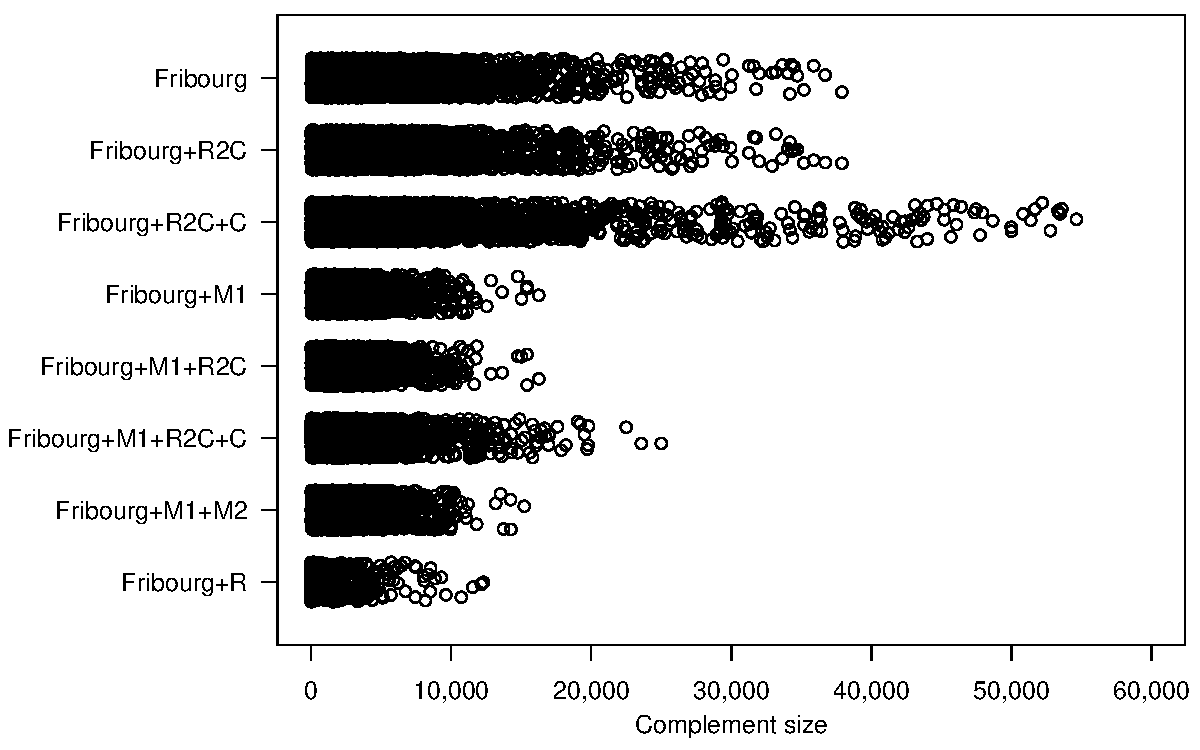
\includegraphics[width=0.7\textwidth]{figures/r/internal/goal/s.stripchart.pdf}
\caption{Stripchart with the complement sizes of the 10,939 effective samples of the \goal{} test set.}
\label{i.g.stripchart}
\end{figure}

The first thing to note is that the distribution of complement sizes is extremely right-skewed (also known as positive-skewed). The peak close to the left end of the x-axis and there is a long tail toward the right. This means that most of the complements are very small and the frequency decreases with increasing complement size. Finally, there are some few complements which are very large. This distribution implies that the mean is generally higher than the median, because the mean is ``dragged'' to the right by the few very large complements.

Next, we can compare the distributions of the individual version to each other. While Fribourg and Fribourg+R2C have a similarly long tail, Fribourg+R2C+C has a considerably longer one. This clearly is the effect of increasing the size of 91\% of the automata by adding a sink state in order to make them complete. Next, Fribourg+M1, Fribourg+M1+M2, and Fribourg+M1+R2C have similarly long tails that are significantly shorter than the ones of the previous versions. This indicates that the M1 optimisation is effective in reducing the size of otherwise large complements. Fribourg+M1+R2C+C, as expected, again increases the size of the tail due to the C option. Finally, Fribourg+R has a very short tail and an even higher concentration of very small complements. This is because the complements are pruned by removing their unreachable and dead states, and thus at least the complements of the 61.8\% universal input automata are reduced to empty automata of size 1.

Having a first impression of the distribution of complement sizes, we can look at some statistics characterising this distribution. Table~\ref{i.g.stats_table} shows the mean complement size along with the classic five-number summary consisting of minimum value, 25th percentile, median, 75th percentile and maximum value for each version of the Fribourg construction. As expected, the mean is always higher than the median. Generally, the median is a more robust metrics than the mean, because it is not affected by the value of outliers. This applies specifically to our distribution where some few very large complements might significantly increase the man whereas they leave the median unaffected. Therefore, the median will be our main metric, and the subsequent analyses will be based on the median.

\begin{table}[ht]
\centering
% latex table generated in R 3.1.2 by xtable 1.7-4 package
% Sat Jun  6 16:42:20 2015
\begin{tabular}{lrrrrrr}
  \hline
Construction & Mean & Min. & P25 & Median & P75 & Max. \\ 
  \hline
Piterman+EQ+RO & 209.6 & 1 & 38.0 & 80.0 & 183.0 & 20,349 \\ 
  Slice+P+RO+MADJ+EG & 949.4 & 2 & 120.0 & 396.0 & 1,003.0 & 41,081 \\ 
  Fribourg+M1+R2C & 1,017.3 & 2 & 153.0 & 452.0 & 1,134.0 & 37,068 \\ 
   \hline
\end{tabular}

\caption{Statistics of the complement sizes of the 10,939 effective samples of the \goal{} test set.}
\label{i.g.stats_table}
\end{table}

Going through the median values in Table~\ref{i.g.stats_table} we encounter some surprises. To begin with, as expected, there is a decrease from Fribourg (761) to Fribourg+R2C (689). Then, however, there is a significant drop to 451 with Fribourg+R2C+C. This is a surprise insofar as by looking at Figure~\ref{i.g.stripchart}, Fribourg+R2C+C seems to have the worst performance at a first glance. Indeed it also has the highest mean, which is due to the group of extremely large complements. The median, however, is very low, even lower than the one of Fribourg+M1 with its significantly shorter tail in Figure~\ref{i.g.stripchart}. Also the 25th percentile of Fribourg+R2C+C is with 85 one of the lowest. Going to the other side of the median, however, the 75th percentile (2,329) is the largest of all versions. A possible characterisation of this phenomenon is that the C option (together with R2C) makes small complements smaller, and large complements larger. The diminishment of small complements is far-reaching enough that the median is affected by it and decreased significantly.

The next thing we see in Table~\ref{i.g.stats_table} is that the median of Fribourg+M1 (482) is slightly lower than the median of Fribourg+M1+M2 (496). The same applies to the 25th and 75th percentile. This backs up our statement from Section~\ref{4_internal} that Fribourg+M1 performs better on the \goal{} teset set than Fribourg+M1+M2. The difference is rather small (the median increase is by 2.9\%), but it is enough to consider Fribourg+M1 as the better of the two versions, and to combine it therefore with R2C and R2C+C.

Fribourg+M1+R2C brings down the median from 482 to 447, with respect to Fribourg+M1. Also the 25th and 75th percentile are decreased. Adding the C option to Fribourg+M1+R2C, again causes the median to drop dramatically, from 447 to 331. The 25th percentile decreases from 152 to 83. The 75th percentile however increases from 1,118 to 1,208.5. Here we have again the same picture of the effecto of adding the C option that we had before. Namely that small complements are made smaller, and large complements are made larger.

Finally, the last row in Table~\ref{i.g.stats_table} with Fribourg+R shows the extent of unreachable and dead states that the Fribourg construction produces. The median is 1, and a further analysis reveals that the single-state complements go up to the 61st percentile. That is, 61\% of the complements have a size of 1. This is likely to correspond to the 61.8\% of universal automata in the GOAL test set whose complements can be reduced to empty automata with a single state.

% Time
% \begin{table}[ht]
% \centering
% % latex table generated in R 3.1.2 by xtable 1.7-4 package
% Wed Aug 19 09:24:28 2015
\begin{tabular}{LrrrrrrRr}
  \hline
Construction & Mean & Min. & P25 & Median & P75 & Max. & Total & $\approx$ hours \\ 
  \hline
Fribourg & 8.5 & 2.5 & 3.3 & 4.9 & 7.3 & 586.0 & 93,351.2 & 259 \\ 
  Fribourg+R2C & 6.6 & 2.2 & 2.9 & 4.2 & 6.4 & 219.7 & 72,545.7 & 202 \\ 
  Fribourg+R2C+C & 8.5 & 2.2 & 2.6 & 3.5 & 6.4 & 582.9 & 93,396.2 & 259 \\ 
  Fribourg+M1 & 4.9 & 2.5 & 3.2 & 4.1 & 5.9 & 55.1 & 54,061.3 & 150 \\ 
  Fribourg+M1+R2C & 4.4 & 2.2 & 2.8 & 3.6 & 5.3 & 42.5 & 48,572.0 & 135 \\ 
  Fribourg+M1+R2C+C & 5.6 & 2.5 & 3.2 & 4.0 & 6.5 & 147.4 & 60,918.9 & 169 \\ 
  Fribourg+M1+M2 & 4.6 & 2.2 & 2.9 & 3.8 & 5.1 & 38.4 & 49,848.0 & 138 \\ 
  Fribourg+R & 7.5 & 2.2 & 3.0 & 3.9 & 6.3 & 470.5 & 82,387.3 & 229 \\ 
   \hline
\end{tabular}

% \caption{Running times in seconds of the complementation tasks, measured as CPU time.}
% \end{table}
% \textcolor{red}{It is strange that Fribourg+R is so much faster than Fribourg}

Up to now, we only looked at statistics aggregated over the entire test set. But as we know from Section~\ref{4_goal_testset}, the 11,000 automata of the \goal{} test set are divided into 110 classes which consist of combinations of 11 transition densities and 10 acceptance densities. The transition densities range from 1 to 3 in steps of 0.2, and the acceptance densities range from 0.1 to 1 in steps of 0.1. In each class there are 100 automata. It is assumable that the median complement sizes are different for different classes. In the next step of the analysis, we want to analyse exactly this point. How do the median complement sizes of the different classes compare to each other, and can we identify a pattern of the classes that result in large and small complements?

This type of analysis naturally results in three-dimensional data. The classes themselves have two dimensions (the transition densities and the acceptance densities), and each of them has a third dimension consisting of the median complement size of this class. One way to present such data is by, for example, a 11x10 matrix with the rows being the transition densities, the columns the acceptance densities, and the cells the median values. Another way is by so called perspective plots. We used both of these ways in Section~\ref{4_goal_testset} when we analysed the number of complete and universal automata in each class of the \goal{} test set. In the present analysis, we will use perspective plots and omit the matrices for space reasons. However, we present the corresponding matrices in Appendix~\ref{app_matrices}. In this way, the interested reader may consult the exact values of the median complement sizes for each class. In the same way, we restrict ourselves to the median complement sizes as the third dimension. The same analysis could also be done, for example, for the mean, the 25th percentile, or the 75th percentile of complement sizes. However, as mentioned, we consider the median to be the most meaningful statistics, and thus exclusively focus on it for the matter of conciseness.

Figures~\ref{i.g.persp-1} and~\ref{i.g.persp_2} show the perspective plots of the median complement sizes for the 110 classes of the \goal{} test set. Each crossing of two lines on the xy-plane represents a class, and the z-value (height) of thie crossing indicates the median complement size of this class. As a help for the orientation, if one imagines the corresponding matrices, as they are presented in Appendix~\ref{app_matrices}, then in the perspective plots we are looking at these matrices from the bottom-right corner. That is, the class that is in the top-left corner of a matrix (transiton density 1.0 and acceptance density 0.1) is the one that is the farthest away from the viewer in the corresponding perspective plot. This orientation holds for all the remaining perspective plots in this thesis. The colours of the squares in the perspective plot (called facets) are a function of the z-values of their four corners and are selected to draw an analogy with topographical terrain maps.

\newcommand{\perspwidth}{0.475}

\begin{figure}[ht]
\centering
  \hfill
  \begin{subfigure}[t]{\perspwidth\textwidth}
  \centering
  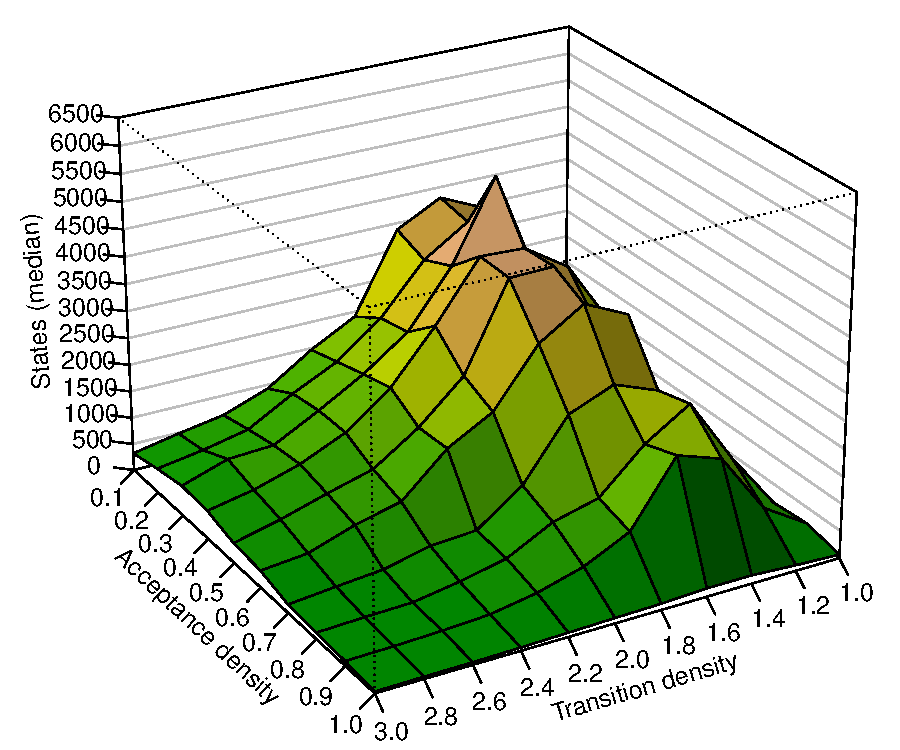
\includegraphics[width=\textwidth]{figures/r/internal/goal/s.median.Fribourg.pdf}
  \caption{Fribourg}
  \end{subfigure}
  \hfill
  \begin{subfigure}[t]{\perspwidth\textwidth}
  \centering
  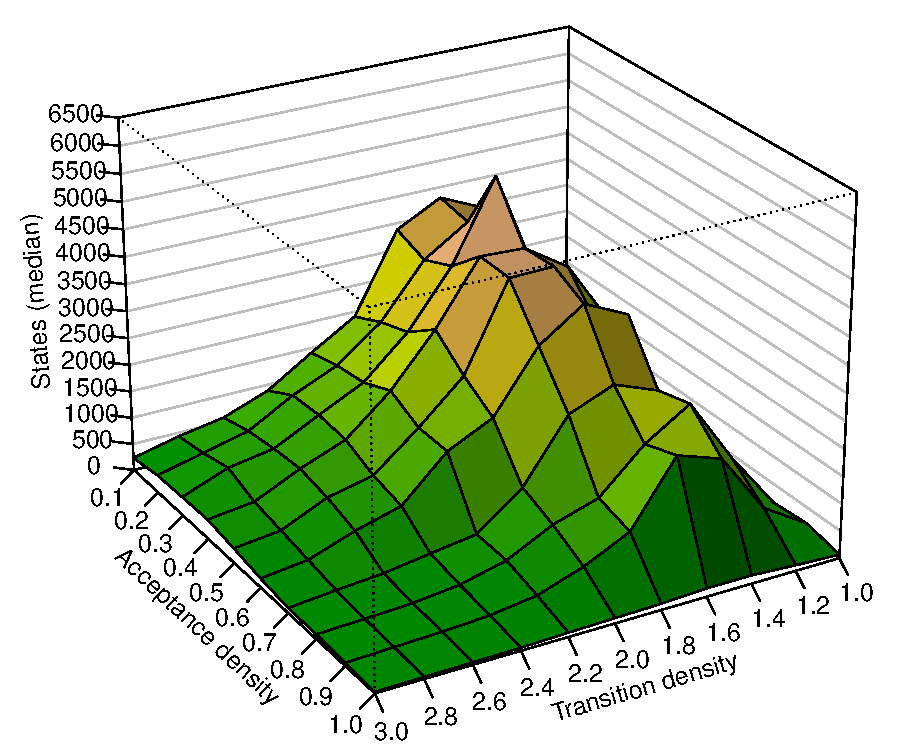
\includegraphics[width=\textwidth]{figures/r/internal/goal/s.median.Fribourg+R2C.pdf}
  \caption{Fribourg+R2C}
  \end{subfigure}
  \hfill

  \hfill
  \begin{subfigure}[t]{\perspwidth\textwidth}
  \centering
  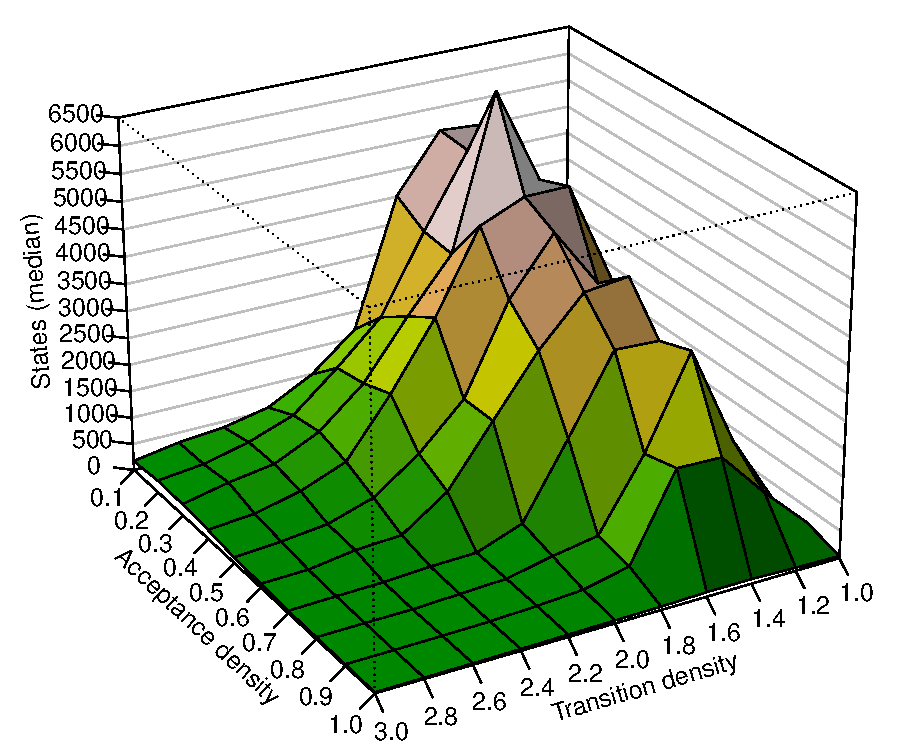
\includegraphics[width=\textwidth]{figures/r/internal/goal/s.median.Fribourg+R2C+C.pdf}
  \caption{Fribourg+R2C+C}
  \end{subfigure}
  \hfill
  \begin{subfigure}[t]{\perspwidth\textwidth}
  \centering
  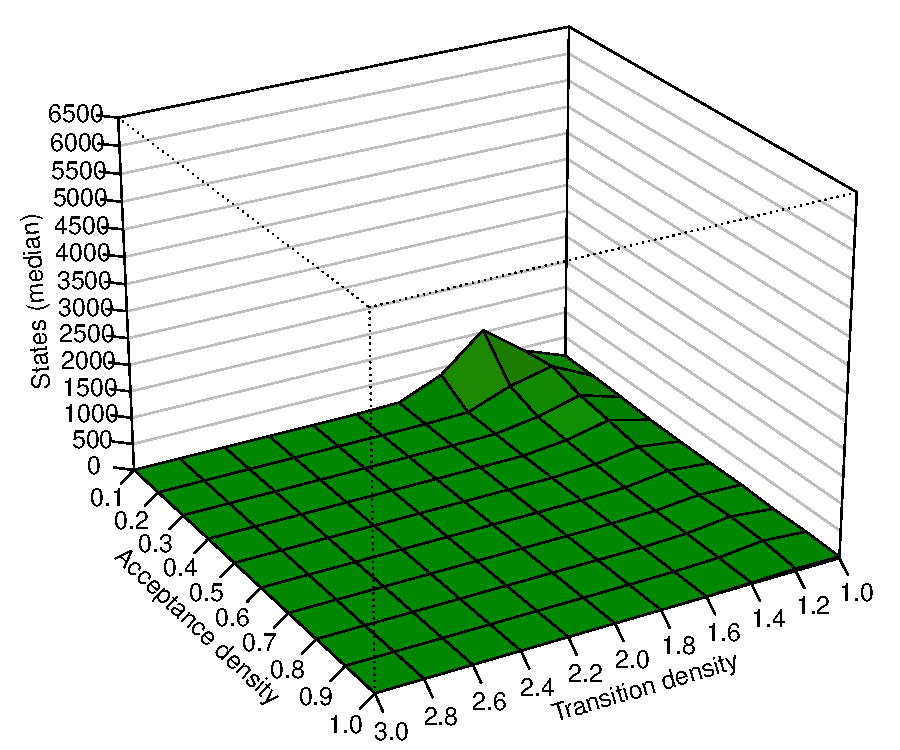
\includegraphics[width=\textwidth]{figures/r/internal/goal/s.median.Fribourg+R.pdf}
  \caption{Fribourg+R}
  \end{subfigure}
  \hfill  
\caption{Median complement sizes of the 110 transition density/acceptance density classes of the 10,939 effective samples of the \goal{} test set.}
\label{i.g.persp_1}
\end{figure}

The first thing we notice when looking at the plots in Figure~\ref{i.g.persp_1} and~\ref{i.g.persp_2} is that there are indeed large differences in the median complement sizes across the transition/acceptance density classes. Figuratively speaking, there is an oblong mountain (or hill) in the northern part of the area in east-west orientation, whose ridge increases in height from east to west and stays high until the western edge of the area. The mountain is located roughly in the area of transition densities between 1.2 and 2.2 and acceptance densities from 0.1 up to 0.9. This means that the automata of these classes are apparently harder to complement than the automata of other classes, as they result more frequently in larger complements.

We will further elaborate on the reasons of these different complement sizes across classes, and also try to characterise easy, medium, and hard automata for the Fribourg construction, at the end of this subsection. For now, we focus on the relative differences of median complement sizes between the different versions of the Fribourg construction.

Looking at Figure~\ref{i.g.persp_1}, the perspective plots for Fribourg and Fribourg+R2C are rather similar. The top of the mountain ridge is at between 3,500 and 4,000 states with a single peak of around 4900 states in the class with transition density 1.6 and acceptance density 0.3. From Table~\ref{i.g.stats_table} we can learn that the overall median complement size is 761 for Fribourg and 689 for Fribourg+R2C. These low values might surprise at first as the mountain, which is much higher, seems to dominate. However, by taking a closer look, it becomes apparent that around half of the classes are in rather low terrain (less than 1,000 states). Furthermore, the heights of the mountain peak do not allow to deduce anything about the overall median, because the median is not affected by the actual values of the data points which are greater than the median. This is the main characteristics of the median and applies to all the subsequent perspective plots in this chapter. The means in turn are 2,004.6 for Fribourg and 1955.9 for Fribourg+R2C.

Fribourg+R2C+C in Figure~\ref{i.g.persp_1} (c) has an even considerably higher mountain than the previous two versions. The top of the ridge is at around 5,000 states and the peak at the class with transition density 1.6 and acceptance density 0.3 has close to 6,500 states. This increase in height is however not reflected in the overall median of Fribourg+R2C+C relative to Fribourg+R2C. As we have seen in in Table~\ref{i.g.stats_table}, the median of Fribourg+R2C+C is 451, and thus 34.5\% lower than the median of Fribourg+R2C. By taking a closer look at the perspective plots, the reason for this can be seen, as the low areas of Fribourg+R2C+C are indeed slightly lower than the low areas of Fribourg+R2C. The significantly higher high areas of Fribourg+R2C+C do not have an effect on the overall median. However, they do have an effect on the overall mean which with 2,424.6 is indeed 24\% higher than the one of Fribourg+R2C (1,955.9).

Going from the first three perspective plot in Figure~\ref{i.g.persp_1} to the perspective plot of Fribourg+R is like going from the Swiss Alps to a Dutch polder. The mountain shrinks to a small hillock and the rest of the terrain is low and flat. This is because so many complements of the Fribourg construction can be reduced to very small sizes by removing their unreachable and dead states. A look at the corresponding matrix in Appendix~\ref{app_matrices} reveals that 68 of the 110 classes have a median complement size of 1. If we further compare this matrix to the matrix with the number of universal automata in Figure~\ref{4_compl_univ} (b), we see that all the classes with a median of 1 contain more than 50 universal automata, and the classes with a median greater than 1 contain less than 50 universal automata. There is a total of 100 automata per class. This makes sense as the complements of universal automata are empty automata, and every empty automaton can be reduced to an automaton with a single non-accepting state. Looking at the classes with a median greater than 1, we see that their values are still considerably lower than the ones of the plain Fribourg construction, which indicates that the Fribourg construction generates a large number of unreachable and dead states. However, as already mentioned, this thread of analysis is not the focus of the present thesis, and we leave it for future work.

\begin{figure}[ht]
\centering
  \hfill
  \begin{subfigure}[t]{\perspwidth\textwidth}
  \centering
  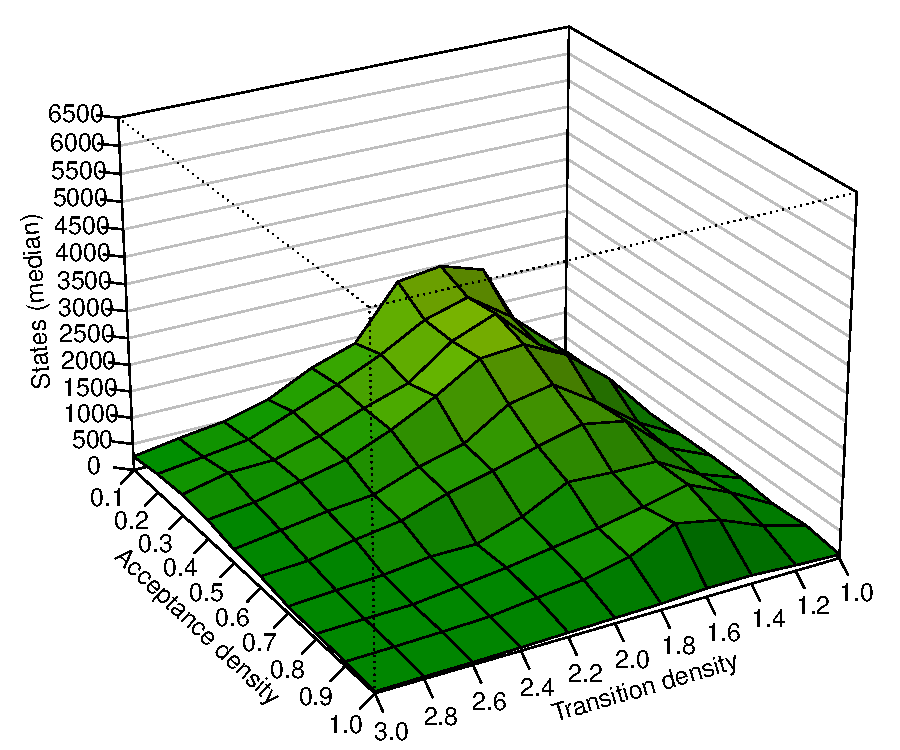
\includegraphics[width=\textwidth]{figures/r/internal/goal/s.median.Fribourg+M1.pdf}
  \caption{Fribourg+M1}
  \end{subfigure}
  \hfill
  \begin{subfigure}[t]{\perspwidth\textwidth}
  \centering
  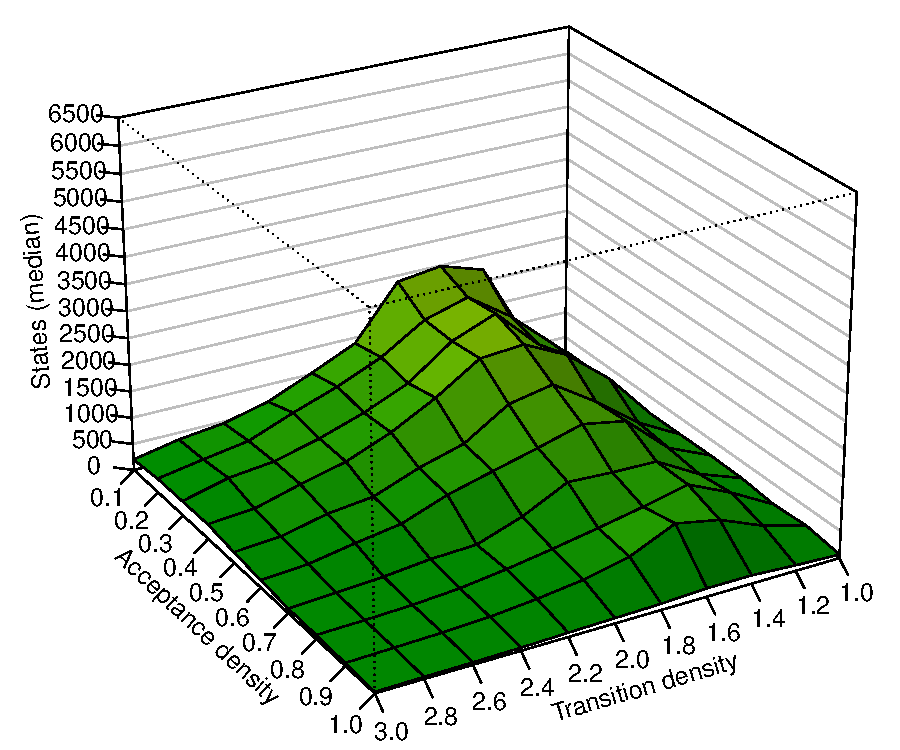
\includegraphics[width=\textwidth]{figures/r/internal/goal/s.median.Fribourg+M1+R2C.pdf}
  \caption{Fribourg+M1+R2C}
  \end{subfigure}
  \hfill

  \hfill
  \begin{subfigure}[t]{\perspwidth\textwidth}
  \centering
  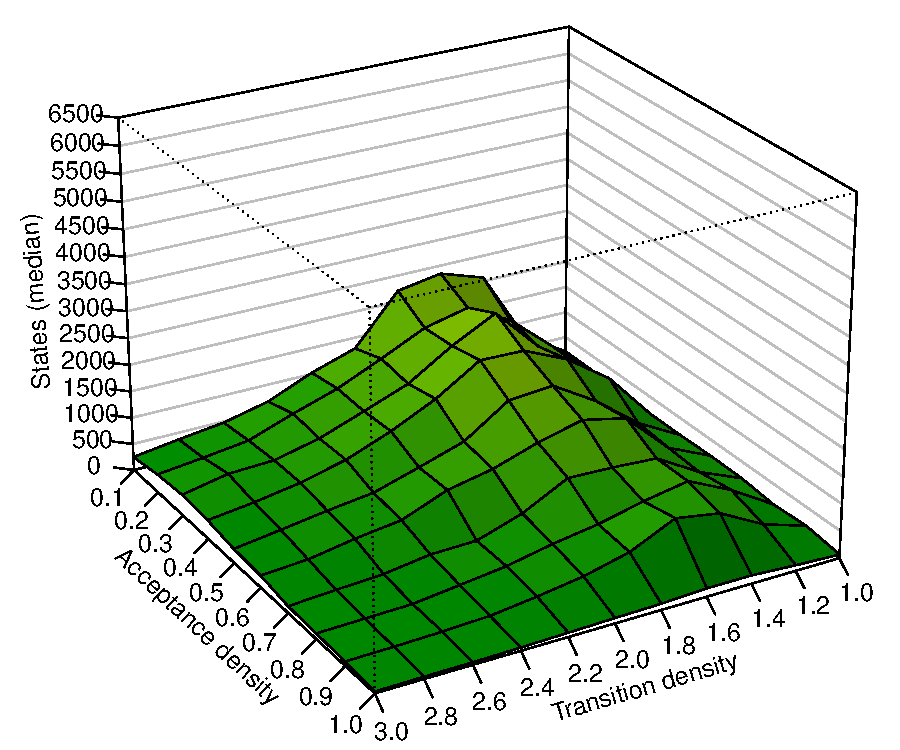
\includegraphics[width=\textwidth]{figures/r/internal/goal/s.median.Fribourg+M1+M2.pdf}
  \caption{Fribourg+M1+M2}
  \end{subfigure}
  \hfill
  \begin{subfigure}[t]{\perspwidth\textwidth}
  \centering
  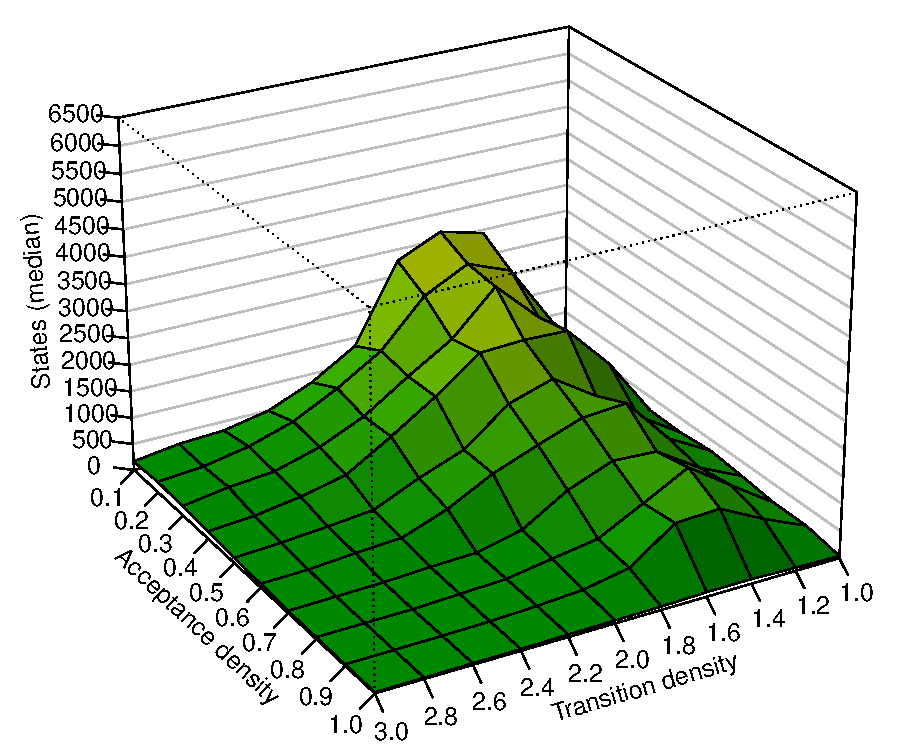
\includegraphics[width=\textwidth]{figures/r/internal/goal/s.median.Fribourg+M1+R2C+C.pdf}
  \caption{Fribourg+M1+R2C+C}
  \end{subfigure}
  \hfill
\label{i.g.persp_2}
\end{figure}

Figure~\ref{i.g.persp_2} shows the perspective plots of the remaining four versions of the Fribourg construction, all of which include the M1 optimisation. The first thing we note is that, while the mountain is still there, its height shrinks significantly. For Fribourg+M1, and Fribourg+M1+R2C, the top of the ridge is between is around 2,500 states. This is reflected by the overall means of these two versions compared to their counterparts without the M1 optimisation, Fribourg, and Fribourg+R2C. The decrease of the overall mean from Fribourg to Fribourg+M1 is by 52\% (from 2004.6 to 963.2) and from Fribourg+R2C to Fribourg+M1+R2C by 52.1\% (from 1955.9 to 937.7). The decreases of the overall medians are by 36.6\% (from 761 to 482), and 35.1\% (from 689 to 447) for the same two pairs of versions. With this we can confirm that the M1 optimisation brings a significant performance gain. 

Regarding the M2 optimisation, we can see that the mountain ridge in the Fribourg+M1+M2 perspective plot is slightly lower than the one in the Fribourg+M1 perspective plot. The flatland regions, however, seem to not change much. This is reflected by the overall mean of Fribourg+M1+M2 which is slightly lower than in Fribourg+M1 (958.9 opposed to 963.2). The overall median, on the other hand, is higher for Fribourg+M1+M2 than for Fribourg+M1 (496 opposed to 482). An interpretation of this behaviour is that the application of the M2 optimisation results in smaller complements for \textit{some} input automata. These automata are especially the ``hard'' ones that produce large complements. This positive effect of M2 does however not affect enough input automata, especially not the ``easy'' automata, as to improve the overall performance of the construction in terms of median complement size. As already stated previously, we consider therefore Fribourg+M1 as the better construction on the \goal{} test set than Fribourg+M1+M2.

Finally,Fribourg+M1+R2C+C differs from Fribourg+M1+R2C in a similar way Fribourg+R2C+C differs from Fribourg+R2C. The higher regions get higher and the lower regions get lower, that is, a performance decline on ``hard'' automata, but a performance gain on easy automata. The performance gain on the easy automata is however effective enough to decrease the overall median from 447 to 331, which is minus 26\%.

With 331 states, Fribourg+M1+R2C+C has the lowest median of all the versions (except Fribourg+R which is a special case because it modifies the output of the construction). However, we still declare Fribourg+M1+R2C as the winner on the \goal{} test set, mainly for two reasons. First, while Fribourg+M1+R2C+C has a lower median, the mean is still higher (1062.6 to 937.7 which is a plus of 13.3\%). This results from the complements of the hard automata, which are larger than with Fribourg+M1+R2C. From a practical point of view, the mean might be relevant, because it relates more directly to the required computing resources than the median. For example the execution CPU time per complementation task, that we also measured along with our experiments, is 25.4\% higher for Fribourg+M1+R2C+C than for Fribourg+M1+R2C. The increase in the average execution time per automaton is from 4.44 to 5.57 seconds and in the total execution time from 48,572 seconds ($\approx$ 135 hours) to 60,919 seconds ($\approx$ 169 hours). Fribourg+M1+R2C, on the other hand, has the lowest mean of all versions. The second reason that we choose Fribourg+M1+R2C as the winner and not Fribourg+M1+R2C+C is that the C option is not a real part of the construction. It actually modifies the input automata before the construction starts in order to make them better suited for the construction. Fribourg+M1+R2C, on the other hand, includes only native options, and input and output of the construction are not modified. This should also make it fairer to compare the Fribourg construction to other constructions in the external tests (Section~\ref{ext}).

As we have seen, there are big difference in the complement sizes across the different classes of the \goal{} test set. Furthermore, there is a certain pattern, namely the mountain in the north-western region of the class matrix. Automata of classes that are in the mountain region seem to be harder to complement than automata from the classes in the flatland region. We attempted to categorise the classes of the \goal{} test set into the three groups ``easy'', ``medium'', and ``hard''. To do so, we first averaged the matrices with the median complement sizes of all the eight versions of the Fribourg construction. In this way, we have a mean median complement size for each class. Then we defined two breakpoints that divide the classes into easy, medium, and hard groups. The breakpoints 500 and 1,600 result in an appropriate groups that seem to capture the reality well. The result with these breakpoints can be seen in Figure~\ref{i.g.difficulty}.

\begin{figure}[ht]
\centering
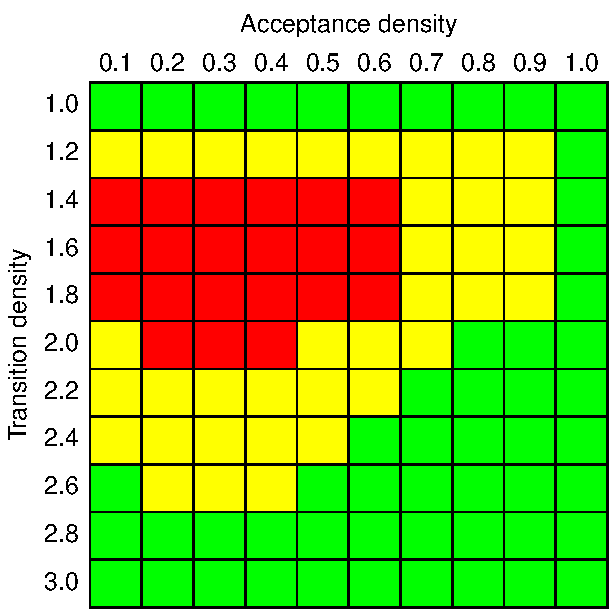
\includegraphics[width=0.35\textwidth]{figures/r/internal/goal/difficulty.pdf}
\caption{Difficulty categories of the transition/acceptance density classes of the \goal{} test set. Green: easy; yellow: medium; red: hard.}
\end{figure}

As can be seen in Figure~\ref{i.g.difficulty}, there are 53 easy, 36 medium, and 21 hard classes. The easy classes are mainly those with extreme values. In particular, all the classes with a low or high transition density of 0.1, or 2.8 and 3.0, and a high acceptance density of 1.0 are easy. Furthermore, there is a ``triangle'' of easy classes between transition densities 2.0 and 2.6. and acceptance densities 0.5 and 0.9. The higher the transition density, the lower the acceptance density may be so that the corresponding class is still easy. The hard classes are roughly those with a transition density between 1.4 and 1.8 and an acceptance density between 0.1 and 0.6. The medium classes finally are situated as a ``belt'' around the hard classes.

It is interesting that the extreme values of transition density and acceptance density result in easy automata. With a transition density of 1.0 and an alphabet size of 2, each of the 15 states has on average two outgoing and two incoming transitions\footnote{The transition density multiplied with the number of states defines the number of transition for each symbol of the alphabet in the automaton, see Section~\ref{4_goal_testset}.}. With a transition density of 3.0, each state has on average 6 outgoing and 6 incoming transitions. These low or high connectivity seems to considerably simplify the complementation task. The same applies to a high acceptance density of 1.0, which means that every state is an accepting state\footnote{The acceptance density defines the percentage of states that are accepting, see Section~\ref{4_goal_testset} as well.}. Generally, we can say that automata with high acceptance densities are easier to complement than automata with lower acceptance densities. This also means that the pattern of easy automata at the extreme values of transition and accceptance density, does not apply to to the lower extreme of the acceptance density. Automata with a very low acceptance density of 0.1 are hard to complement---unless they are made easy by a low or high transition density.

Another interesting point is that the hard automata have transition densities between 1.4 and 1.8. It seems that this range of transition densities is the crucial factor in the hardness of a complementation task, and that it is only alleviated by a growing acceptance density. This explains the decline of the mountain ridge from west to east.

Summarising we can say that transition densities between 1.4 and 1.8 produce the hardest complementation tasks, and that to the both sides the difficulty steadily decreases with declining or growing transition density. Furthermore, a growing acceptance density generally implies easier complementation tasks.


\subsection{Michel Test Set}
We complemented the first four Michel automata with the six versions of the Fribourg constructions that are listed in Section~\ref{4_internal}. All complementation tasks were successful, as we did not set a timeout or memory limit. Remember that the first four Michel automata have 3, 4, 5, and 6 states, respectively. The sizes of the resulting complements are presented in Figure~\ref{i.m.states} in table form and visualised as a grouped barplot.

\begin{table}[ht]
\centering
% latex table generated in R 3.1.2 by xtable 1.7-4 package
% Sun Aug 16 00:19:45 2015
\begin{tabular}{lrrrrrr}
  \hline
Construction & Michel 1 & Michel 2 & Michel 3 & Michel 4 & Fitted curve & Std. error \\ 
  \hline
Fribourg & 57 & 843 & 14,535 & 287,907 & $(1.35n)^n$ & 0.01\% \\ 
  Fribourg+R2C & 33 & 467 & 8,271 & 168,291 & $(1.24n)^n$ & 0.06\% \\ 
  Fribourg+M1 & 44 & 448 & 5,506 & 81,765 & $(1.10n)^n$ & 0.07\% \\ 
  Fribourg+M1+M2 & 42 & 402 & 4,404 & 57,116 & $(1.03n)^n$ & 0.12\% \\ 
  Fribourg+M1+M2+R2C & 28 & 269 & 3,168 & 43,957 & $(0.99n)^n$ & 0.04\% \\ 
  Fribourg+R & 18 & 95 & 528 & 3,315 & $(0.64n)^n$ & 0.35\% \\ 
   \hline
\end{tabular}

\caption{Complement sizes of the first four Michel automata.}
\label{i.m.states}
\end{table}

% \begin{figure}[ht]
%   \centering
%   \begin{subtable}{0.75\textwidth}
%     \centering
%     % latex table generated in R 3.1.2 by xtable 1.7-4 package
% Sun Aug 16 00:19:45 2015
\begin{tabular}{lrrrrrr}
  \hline
Construction & Michel 1 & Michel 2 & Michel 3 & Michel 4 & Fitted curve & Std. error \\ 
  \hline
Fribourg & 57 & 843 & 14,535 & 287,907 & $(1.35n)^n$ & 0.01\% \\ 
  Fribourg+R2C & 33 & 467 & 8,271 & 168,291 & $(1.24n)^n$ & 0.06\% \\ 
  Fribourg+M1 & 44 & 448 & 5,506 & 81,765 & $(1.10n)^n$ & 0.07\% \\ 
  Fribourg+M1+M2 & 42 & 402 & 4,404 & 57,116 & $(1.03n)^n$ & 0.12\% \\ 
  Fribourg+M1+M2+R2C & 28 & 269 & 3,168 & 43,957 & $(0.99n)^n$ & 0.04\% \\ 
  Fribourg+R & 18 & 95 & 528 & 3,315 & $(0.64n)^n$ & 0.35\% \\ 
   \hline
\end{tabular}

%   \end{subtable}

%   \begin{subfigure}{0.7\textwidth}
%     \centering
%     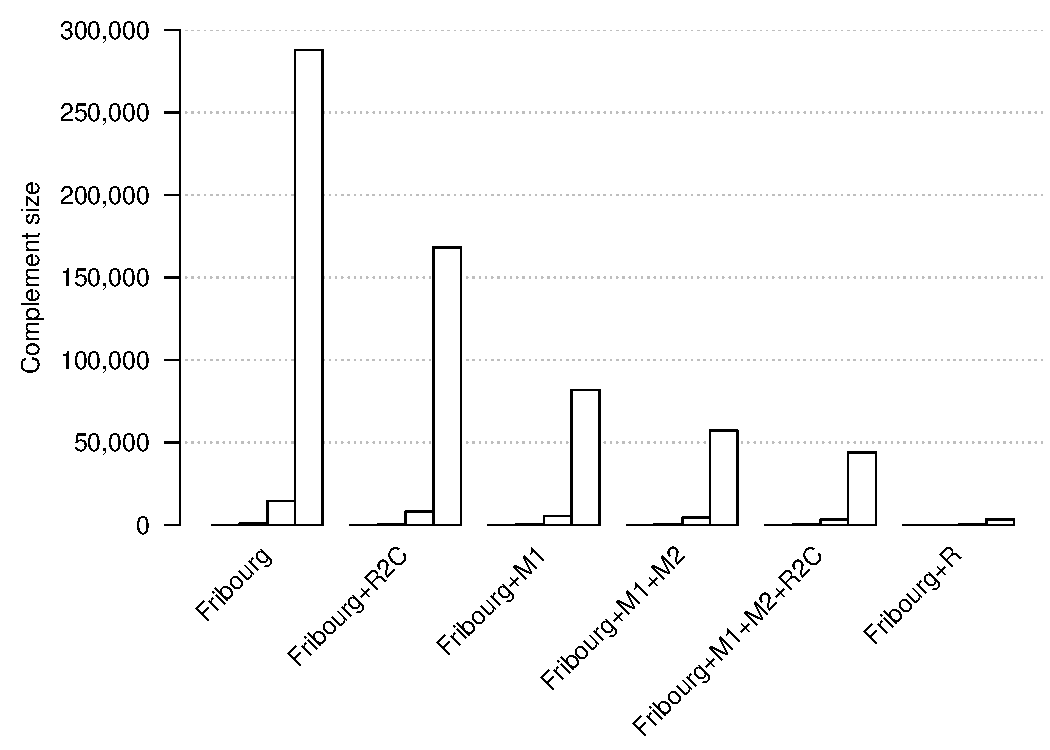
\includegraphics[width=\textwidth]{figures/r/internal/michel/s.barplot.pdf}
%     \caption{Complement sizes of the first four Michel visualised as a barplot. The bars 1 to 4 of each group correspond to Michel automata 1 to 4.}
%   \end{subfigure}
% \caption{Complement sizes of the Michel automata in table form and visualised as a barplot. Each version of the Fribourg construction is represented by four bars, which stand for Michel automata 1 to 4, respectively.}
% \label{i.m.states}
% \end{figure}

Looking at the results reveals two things. First, Michel automata result in very large complements. For example, Michel 4, which has six states, results in a complement with 287,907 states with the plain Fribourg construction. This is a state growth of $(1.354n)^n$. Exactly this state explosion is the aim of Michel automata, which have been developed with the goal to crate a set of automata that is extremely hard to complement.

This also shows why we were only able to complement the first four Michel automata. If we assume the same state growth of $(1.354n)^n$ for the fifth Michel automaton, Michel 5, with seven states, then the complement would have around 6.9 million states. The execution time for Michel 4 with the plain Friboug construction was 100,976 CPU time seconds ($\approx$ 180 hours). If we assume a linear relation between the number of generated states and the execution time, then Michel 5 would have an execution time of more than 2.4 million seconds, which is around 279 days. This estimation is still a very conservative, as the relation between complement size and execution time is not linear but seems to be exponential as well (see table with exeuction times in appendix). 




\section{External Tests}
\label{ext}

\subsection{GOAL Test Set}

\begin{table}[ht]
\centering
% latex table generated in R 3.1.2 by xtable 1.7-4 package
% Sat Jun  6 16:42:17 2015
\begin{tabular}{lrr}
  \hline
Construction & Timeouts & Memory excesses \\ 
  \hline
Fribourg & 48 & 0 \\ 
  Fribourg+R2C & 30 & 0 \\ 
  Fribourg+R2C+C & 54 & 0 \\ 
  Fribourg+M1 & 2 & 0 \\ 
  Fribourg+M1+M2 & 1 & 0 \\ 
  Fribourg+M1+R2C & 1 & 0 \\ 
  Fribourg+M1+R2C+C & 8 & 0 \\ 
  Fribourg+R & 48 & 0 \\ 
   \hline
\end{tabular}

\caption{Number of timeouts and memory excesses.}
\end{table}

\begin{itemize}
\item With Rank
  \begin{itemize}
  \item 7,204 effective samples (3,796 uncompleted tasks, 34.51\%)
  \end{itemize}
\item Without Rank
  \begin{itemize}
  \item 10,998 effective samples (2 uncompleted tasks, 0.02\%)
  \end{itemize}
\end{itemize}


\subsubsection{With Rank}

\begin{figure}[ht]
\centering
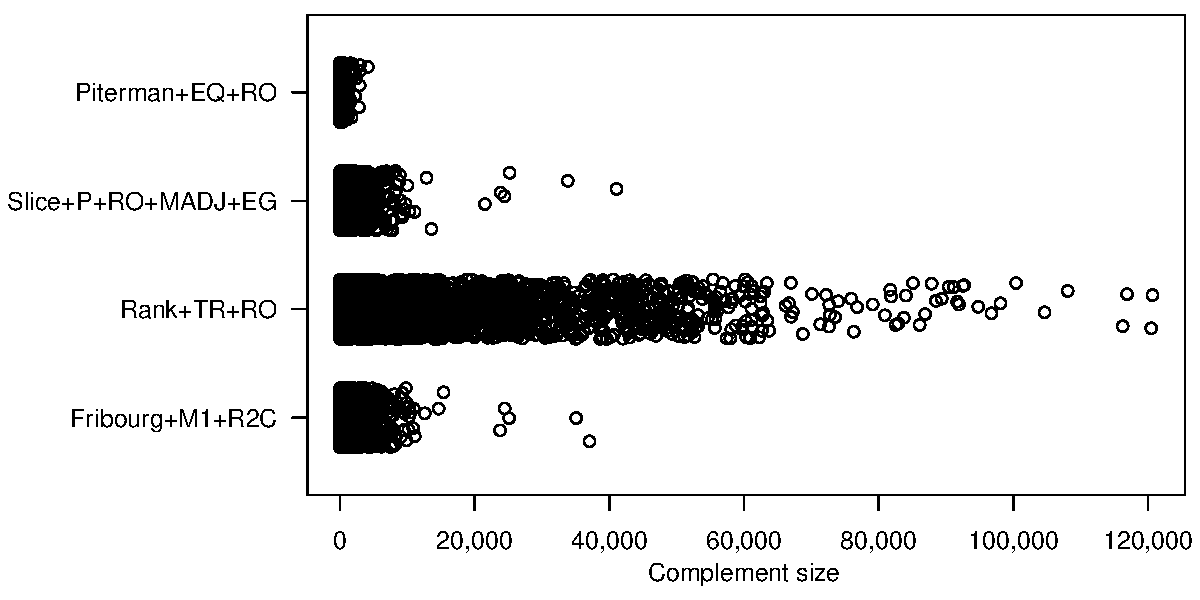
\includegraphics[width=0.75\textwidth]{figures/r/external/goal/s.stripchart.with_rank.pdf}
\caption{Complement sizes of the 7,204 effective samples.}
\end{figure}

\begin{table}[ht]
\centering
% latex table generated in R 3.1.2 by xtable 1.7-4 package
% Sun Aug 16 15:57:19 2015
\begin{tabular}{lrrrrrr}
  \hline
Construction & Mean & Min. & P25 & Median & P75 & Max. \\ 
  \hline
Piterman+EQ+RO & 106.0 & 1 & 29.0 & 58.0 & 121.0 & 4,126 \\ 
  Slice+P+RO+MADJ+EG & 555.4 & 2 & 70.0 & 202.0 & 596.0 & 41,081 \\ 
  Rank+TR+RO & 5,255.6 & 2 & 81.0 & 254.5 & 3,178.2 & 120,674 \\ 
  Fribourg+M1+R2C & 662.9 & 2 & 101.0 & 269.0 & 754.5 & 37,068 \\ 
   \hline
\end{tabular}

\caption{Aggregated statistics of complement sizes of the 7,204 effective samples.}
\end{table}

\begin{table}[ht]
\centering
% latex table generated in R 3.1.2 by xtable 1.7-4 package
% Thu Jun 11 15:11:29 2015
\begin{tabular}{lrrrrrr}
  \hline
Construction & Mean & Min. & P25 & Median & P75 & Max. \\ 
  \hline
Piterman+EQ+RO & 2.97 & 2.22 & 2.58 & 2.78 & 3.03 & 42.93 \\ 
  Slice+P+RO+MADJ+EG & 3.66 & 2.21 & 2.69 & 3.22 & 4.07 & 36.67 \\ 
  Rank+TR+RO & 16.04 & 2.28 & 2.76 & 3.71 & 9.31 & 443.33 \\ 
  Fribourg+M1+R2C & 4.02 & 2.22 & 2.69 & 3.10 & 4.37 & 410.37 \\ 
   \hline
\end{tabular}

\caption{Aggregated statistics of the running times of the 7,204 effective samples.}
\end{table}


\subsubsection{Without Rank}


\begin{figure}[ht]
\centering
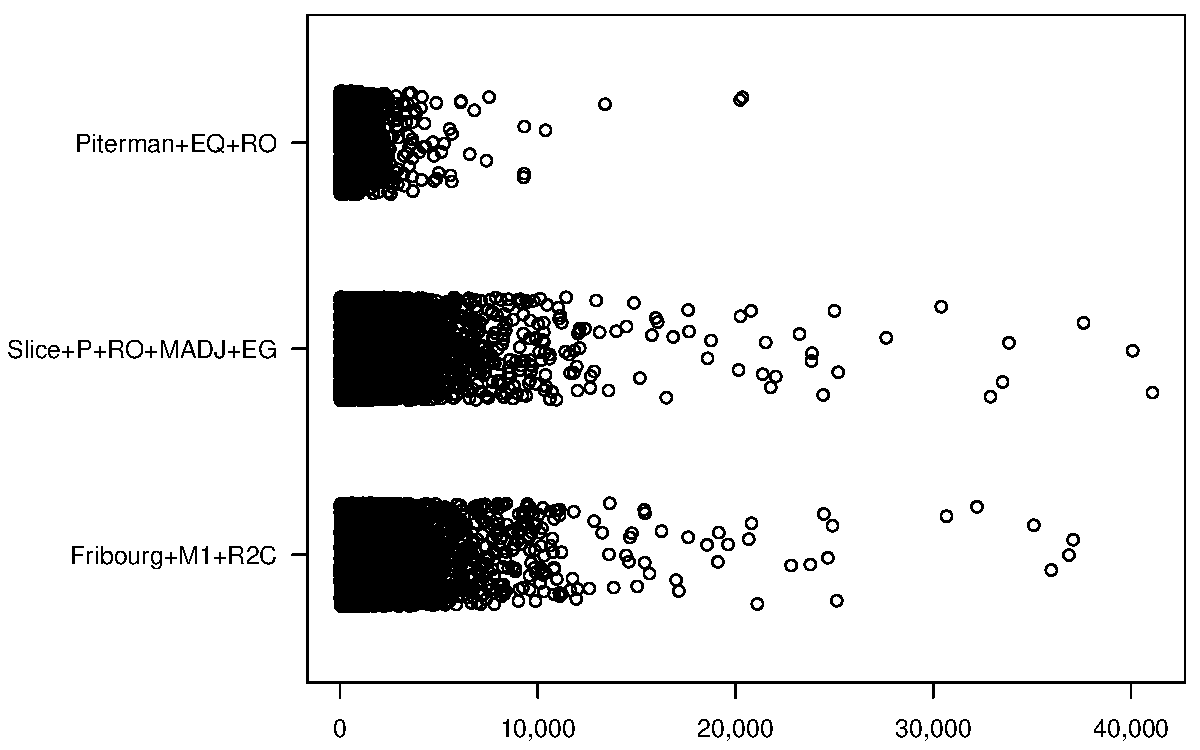
\includegraphics[width=0.75\textwidth]{figures/r/external/goal/s.stripchart.pdf}
\caption{Complement sizes of the 10,998  effective samples.}
\end{figure}


\begin{table}[ht]
\centering
% latex table generated in R 3.1.2 by xtable 1.7-4 package
% Sat Jun  6 16:42:20 2015
\begin{tabular}{lrrrrrr}
  \hline
Construction & Mean & Min. & P25 & Median & P75 & Max. \\ 
  \hline
Piterman+EQ+RO & 209.6 & 1 & 38.0 & 80.0 & 183.0 & 20,349 \\ 
  Slice+P+RO+MADJ+EG & 949.4 & 2 & 120.0 & 396.0 & 1,003.0 & 41,081 \\ 
  Fribourg+M1+R2C & 1,017.3 & 2 & 153.0 & 452.0 & 1,134.0 & 37,068 \\ 
   \hline
\end{tabular}

\caption{Aggregated statistics of complement sizes of the 10,998 effective samples without Rank.}
\end{table}

\begin{table}[ht]
\centering
% latex table generated in R 3.1.2 by xtable 1.7-4 package
% Wed Aug 19 09:24:28 2015
\begin{tabular}{LrrrrrrRr}
  \hline
Construction & Mean & Min. & P25 & Median & P75 & Max. & Total & $\approx$ hours \\ 
  \hline
Fribourg & 8.5 & 2.5 & 3.3 & 4.9 & 7.3 & 586.0 & 93,351.2 & 259 \\ 
  Fribourg+R2C & 6.6 & 2.2 & 2.9 & 4.2 & 6.4 & 219.7 & 72,545.7 & 202 \\ 
  Fribourg+R2C+C & 8.5 & 2.2 & 2.6 & 3.5 & 6.4 & 582.9 & 93,396.2 & 259 \\ 
  Fribourg+M1 & 4.9 & 2.5 & 3.2 & 4.1 & 5.9 & 55.1 & 54,061.3 & 150 \\ 
  Fribourg+M1+R2C & 4.4 & 2.2 & 2.8 & 3.6 & 5.3 & 42.5 & 48,572.0 & 135 \\ 
  Fribourg+M1+R2C+C & 5.6 & 2.5 & 3.2 & 4.0 & 6.5 & 147.4 & 60,918.9 & 169 \\ 
  Fribourg+M1+M2 & 4.6 & 2.2 & 2.9 & 3.8 & 5.1 & 38.4 & 49,848.0 & 138 \\ 
  Fribourg+R & 7.5 & 2.2 & 3.0 & 3.9 & 6.3 & 470.5 & 82,387.3 & 229 \\ 
   \hline
\end{tabular}

\caption{Aggregated statistics of the running times of the 10,998 effective samples without Rank.}
\end{table}

% Persp plots
\renewcommand{\perspwidth}{0.3}

\begin{figure}[ht]
\centering
  \hfill
  \begin{subfigure}[t]{\perspwidth\textwidth}
  \centering
  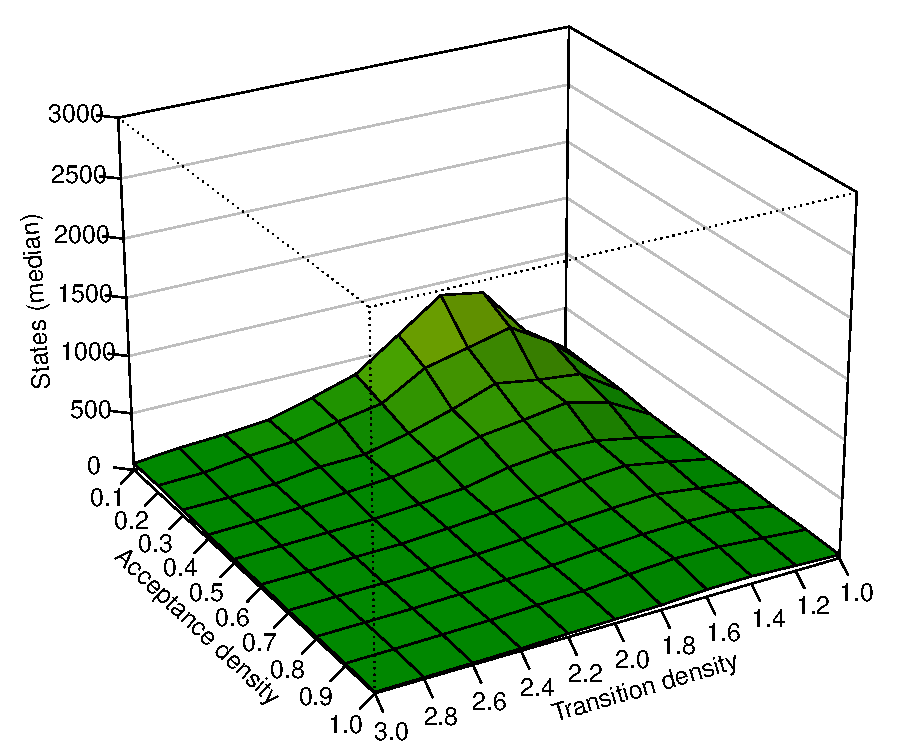
\includegraphics[width=\textwidth]{figures/r/external/goal/s.median.Piterman+EQ+RO.pdf}
  \caption{Piterman+EQ+RO}
  \end{subfigure}
  \hfill
  \begin{subfigure}[t]{\perspwidth\textwidth}
  \centering
  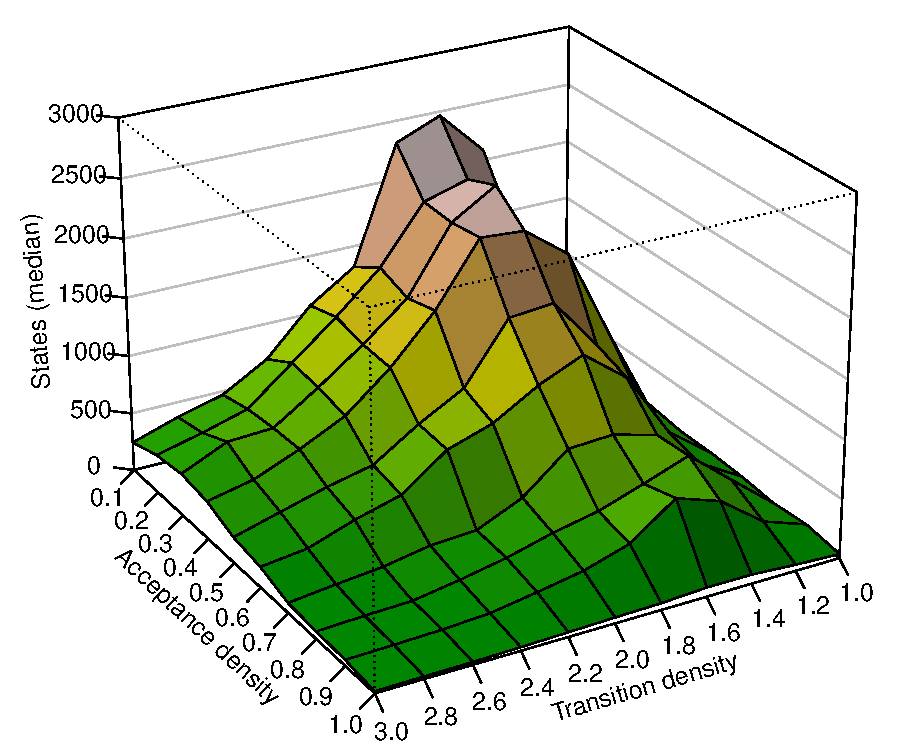
\includegraphics[width=\textwidth]{figures/r/external/goal/s.median.Slice+P+RO+MADJ+EG.pdf}
  \caption{Slice+P+RO+MADJ+EG}
  \end{subfigure}
  \hfill
  \begin{subfigure}[t]{\perspwidth\textwidth}
  \centering
  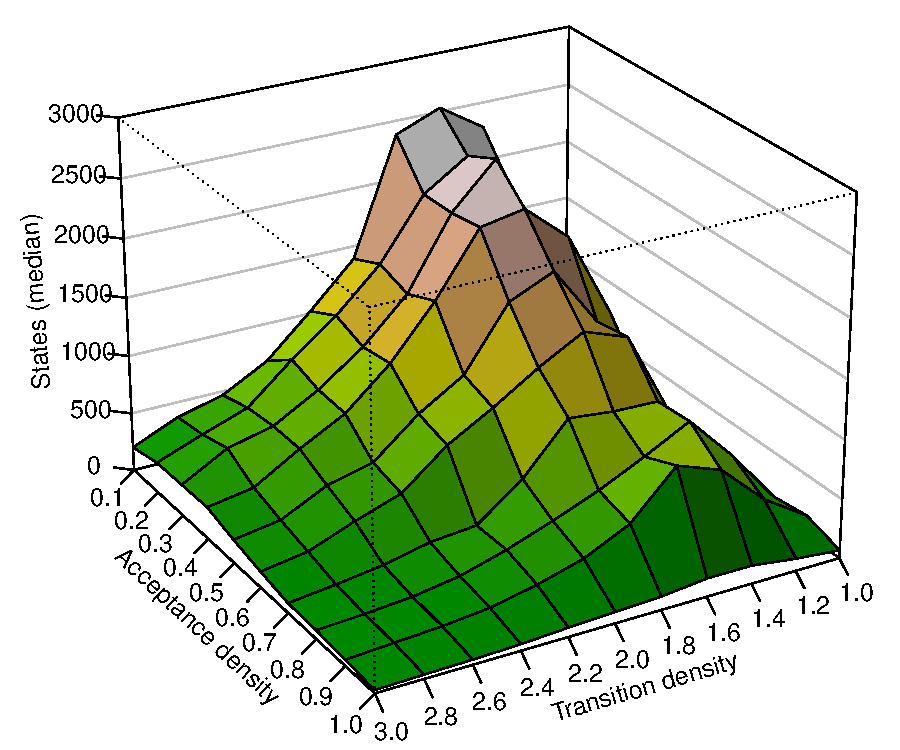
\includegraphics[width=\textwidth]{figures/r/external/goal/s.median.Fribourg+M1+R2C.pdf}
  \caption{Fribourg+M1+R2C}
  \end{subfigure}
  \hfill
\caption{Median complement sizes.}
\end{figure}



\subsection{Michel Automata}




\begin{figure}[ht]
  \centering
  \begin{subtable}{0.75\textwidth}
    \centering
    % latex table generated in R 3.1.2 by xtable 1.7-4 package
% Sun Aug 16 00:19:45 2015
\begin{tabular}{lrrrrrr}
  \hline
Construction & Michel 1 & Michel 2 & Michel 3 & Michel 4 & Fitted curve & Std. error \\ 
  \hline
Fribourg & 57 & 843 & 14,535 & 287,907 & $(1.35n)^n$ & 0.01\% \\ 
  Fribourg+R2C & 33 & 467 & 8,271 & 168,291 & $(1.24n)^n$ & 0.06\% \\ 
  Fribourg+M1 & 44 & 448 & 5,506 & 81,765 & $(1.10n)^n$ & 0.07\% \\ 
  Fribourg+M1+M2 & 42 & 402 & 4,404 & 57,116 & $(1.03n)^n$ & 0.12\% \\ 
  Fribourg+M1+M2+R2C & 28 & 269 & 3,168 & 43,957 & $(0.99n)^n$ & 0.04\% \\ 
  Fribourg+R & 18 & 95 & 528 & 3,315 & $(0.64n)^n$ & 0.35\% \\ 
   \hline
\end{tabular}

    \caption{Complement sizes of the first four Michel automata.}
  \end{subtable}

  \begin{subfigure}{0.75\textwidth}
    \centering
    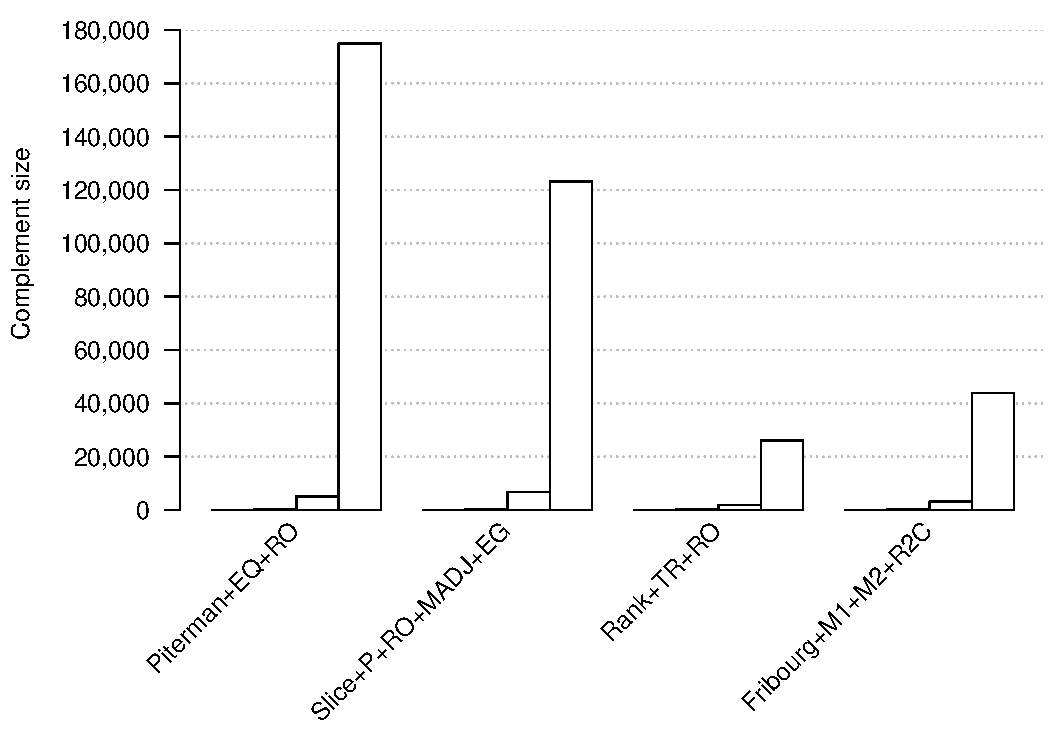
\includegraphics[width=\textwidth]{figures/r/external/michel/s.barplot.pdf}
    \caption{Complement sizes of the first four Michel visualised as a barplot. The bars 1 to 4 of each group correspond to Michel automata 1 to 4.}
  \end{subfigure}
  \caption{Complement sizes of Michel automata.}
\end{figure}


\begin{table}[ht]
\centering
% latex table generated in R 3.1.2 by xtable 1.7-4 package
% Sun Aug 16 00:19:45 2015
\begin{tabular}{lrrrrrr}
  \hline
Construction & Michel 1 & Michel 2 & Michel 3 & Michel 4 & Fitted curve & Std. error \\ 
  \hline
Fribourg & 57 & 843 & 14,535 & 287,907 & $(1.35n)^n$ & 0.01\% \\ 
  Fribourg+R2C & 33 & 467 & 8,271 & 168,291 & $(1.24n)^n$ & 0.06\% \\ 
  Fribourg+M1 & 44 & 448 & 5,506 & 81,765 & $(1.10n)^n$ & 0.07\% \\ 
  Fribourg+M1+M2 & 42 & 402 & 4,404 & 57,116 & $(1.03n)^n$ & 0.12\% \\ 
  Fribourg+M1+M2+R2C & 28 & 269 & 3,168 & 43,957 & $(0.99n)^n$ & 0.04\% \\ 
  Fribourg+R & 18 & 95 & 528 & 3,315 & $(0.64n)^n$ & 0.35\% \\ 
   \hline
\end{tabular}

\caption{Execution times for the first four Michel automata.}
\end{table}


% \chapter{Conclusions}
% \label{chap_conclusions}
% \newpage
% \chapter{Conclusions}

% \appendix
% \chapter{Plugin Installation and Usage}
% \label{appendix_a}
% \input{chapters/appendix_a.tex}



\bibliographystyle{styles/bibstyle}
\bibliography{../bib/buchi_compl}


% Drawings
\begin{figure}
\begin{center}
\Automaton
\end{center}
\end{figure}

\begin{figure}
\begin{center}
\RunTree
\end{center}
\end{figure}

\begin{figure}
\begin{center}
\SubsetConstructionTree
\end{center}
\end{figure}

\begin{figure}
\begin{center}
\SplitTreeRightLeft
\end{center}
\end{figure}

\begin{figure}
\begin{center}
\ReducedSplitTreeRightLeft
\end{center}
\end{figure}

\begin{figure}
\begin{center}
\RunDAG
\end{center}
\end{figure} 

\end{document}
